% All fonts, including those for sub- and superscripts, must be 10
% points or larger.  Recommended sizes are 14-point for chapter
% headings, 12-point for the main body of text and figure/table
% titles, and 10-point for footnotes, sub- and super-scripts, and text
% in figures and tables.
%
% Notes: Add short title to figures, sections, via square brackets,
% e.g. \section[short]{long}.
%
%\documentclass[12pt,fleqn]{style/ucithesis}
\documentclass[12pt]{style/ucithesis}

% A few common packages
\usepackage{amsmath}
\usepackage{amsthm}
\usepackage{array}
\usepackage{graphicx}
\usepackage{relsize}

% Some other useful packages
\usepackage{caption}
\usepackage{subcaption}  % \begin{subfigure}...\end{subfigure} within figure
\usepackage{multirow}
\usepackage{tabularx}

% plainpages=false fixes the "duplicate ignored" error with page counters
% Set pdfborder to 0 0 0 to disable colored borders around PDF hyperlinks
\usepackage[plainpages=false,pdfborder={0 0 0}]{hyperref}
\usepackage{epigraph}
\setlength\epigraphrule{0pt}

\usepackage[sorting=none,hyperref,backend=biber,backref,backrefstyle=none]{biblatex}
\bibliography{bib/references.bib,
                bib/chapter2.bib}

\usepackage{tabularx}
\usepackage{booktabs}

\usepackage{array}
\usepackage{makecell}
\usepackage{graphicx}
\usepackage{arydshln}
\usepackage{stackengine}
\usepackage{xcolor}
\usepackage{amsmath}
\usepackage{placeins}
\usepackage{mathtools}


%\usepackage[sorting=none]{biblatex}
%\addbibresource{bib/references.bib}

% Uncomment the following two lines to use the algorithm package,
% which provides an algorithm environment similar to figure and table
% ("\begin{algorithm}...\end{algorithm}"). A list of algorithms will
% automatically be added in the preliminary pages. Note that you
% probably want a package for the actual code to go with this (e.g.,
% algorithmic).
%\usepackage{algorithm}
%\renewcommand{\listalgorithmname}{\protect\centering\protect\Large LIST OF ALGORITHMS}

% Uncomment the following line to enable Unicode support. This will allow you
% to enter non-ASCII characters (such as accented characters) directly without
% having to use LaTeX's awkward escape syntax (e.g., \'{e})
% NOTE: You may have to install the ucs.sty package for this to work. See:
% http://www.unruh.de/DniQ/latex/unicode/
%\usepackage[utf8x]{inputenc}

% Uncomment the following to avoid "widowing", where page breaks cause
% single lines of paragraphs to float onto the next page (this is not
% a UCI requirement but more of an aesthetic choice).
%\widowpenalty=10000
%\clubpenalty=10000

% Modify or extend these at will.
\newtheorem{theorem}{\textsc{Theorem}}[chapter]
\newtheorem{definition}{\textsc{Definition}}[chapter]
\newtheorem{example}{\textsc{Example}}[chapter]

% Macros for title, author, abstract, etc.
%\thesistitle{
%    Sweet Little Nothings: Searching for a Pairs of Supersymmetric Tops,
%        a Pair of Higgs Bosons, and a Pair of New Small Wheels for the 
%        Upgrade of the ATLAS Forward Muon System
%}

\thesistitle{
Sweet Little Nothings; or, Searching for a Pair of Stops, a Pair of Higgs Bosons,
and a Pair of New Small Wheels for the Upgrade of the Forward Muon System of the
ATLAS Detector at CERN
}

%"Dissertation" for PhD, "Thesis" for master's
\documenttitle{Dissertation}

\degreename{Doctor of Philosophy}

% Use the wording given in the official list of degrees awarded by UCI:
% http://www.rgs.uci.edu/grad/academic/degrees_offered.htm
\degreefield{
Physics
}

% Your name as it appears on official UCI records.
\authorname{
Daniel Joseph Antrim
}

% Use the full name of each committee member.
\committeechair{Professor Anyes Taffard}
\othercommitteemembers
{
  Professor Daniel Whiteson\\
  Professor Arvind Rajaraman
}

\degreeyear{2019}

\copyrightdeclaration
{
  {\copyright} {\Degreeyear} \Authorname
}

% If you have previously published parts of your manuscript, you must list the
% copyright holders; see Section 3.2 of the UCI Thesis and Dissertation Manual.
% Otherwise, this section may be omitted.
% \prepublishedcopyrightdeclaration
% {
% 	Chapter 4 {\copyright} 2003 Springer-Verlag \\
% 	Portion of Chapter 5 {\copyright} 1999 John Wiley \& Sons, Inc. \\
% 	All other materials {\copyright} {\Degreeyear} \Authorname
% }

% The dedication page is optional
% (comment out to exclude).
\dedications
{
  (Optional dedication page)
  
  To ...
}

\acknowledgments
{
  I would like to thank...
  
  (You must acknowledge grants and other funding assistance. 
  
  You may also acknowledge the contributions of professors and
  friends.
  
  You also need to acknowledge any publishers of your previous
  work who have given you permission to incorporate that work
  into your dissertation. See Section 3.2 of the UCI Thesis and
  Dissertation Manual.)
}


% Some custom commands for your list of publications and software.
\newcommand{\mypubentry}[3]{
  \begin{tabular*}{1\textwidth}{@{\extracolsep{\fill}}p{4.5in}r}
    \textbf{#1} & \textbf{#2} \\ 
    \multicolumn{2}{@{\extracolsep{\fill}}p{.95\textwidth}}{#3}\vspace{6pt} \\
  \end{tabular*}
}
\newcommand{\mysoftentry}[3]{
  \begin{tabular*}{1\textwidth}{@{\extracolsep{\fill}}lr}
    \textbf{#1} & \url{#2} \\
    \multicolumn{2}{@{\extracolsep{\fill}}p{.95\textwidth}}
    {\emph{#3}}\vspace{-6pt} \\
  \end{tabular*}
}

% Include, at minimum, a listing of your degrees and educational
% achievements with dates and the school where the degrees were
% earned. This should include the degree currently being
% attained. Other than that it's mostly up to you what to include here
% and how to format it, below is just an example.
%
% CV is required for PhD theses, but not Master's
% comment out to exclude
\curriculumvitae
{

\textbf{EDUCATION}
  
  \begin{tabular*}{1\textwidth}{@{\extracolsep{\fill}}lr}
    \textbf{Doctor of Philosophy in Computer Science} & \textbf{2012} \\
    \vspace{6pt}
    University name & \emph{City, State} \\
    \textbf{Bachelor of Science in Computational Sciences} & \textbf{2007} \\
    \vspace{6pt}
    Another university name & \emph{City, State} \\
  \end{tabular*}

\vspace{12pt}
\textbf{RESEARCH EXPERIENCE}

  \begin{tabular*}{1\textwidth}{@{\extracolsep{\fill}}lr}
    \textbf{Graduate Research Assistant} & \textbf{2007--2012} \\
    \vspace{6pt}
    University of California, Irvine & \emph{Irvine, California} \\
  \end{tabular*}

\vspace{12pt}
\textbf{TEACHING EXPERIENCE}

  \begin{tabular*}{1\textwidth}{@{\extracolsep{\fill}}lr}
    \textbf{Teaching Assistant} & \textbf{2009--2010} \\
    \vspace{6pt}
    University name & \emph{City, State} \\
  \end{tabular*}

\pagebreak

\textbf{REFEREED JOURNAL PUBLICATIONS}

  \mypubentry{Ground-breaking article}{2012}{Journal name}

\vspace{12pt}
\textbf{REFEREED CONFERENCE PUBLICATIONS}

  \mypubentry{Awesome paper}{Jun 2011}{Conference name}
  \mypubentry{Another awesome paper}{Aug 2012}{Conference name}

\vspace{12pt}
\textbf{SOFTWARE}

  \mysoftentry{Magical tool}{http://your.url.here/}
  {C++ algorithm that solves TSP in polynomial time.}

}

% The abstract was previously limited to a maximum of 350 words, 
% but the UCI manual at https://etd.lib.uci.edu/electronic/td2e#2.2.1.
% currently does not indicate that there is any word limit for the abstract
\thesisabstract
{
  The abstract of your contribution goes here.
}


%%% Local Variables: ***
%%% mode: latex ***
%%% TeX-master: "thesis.tex" ***
%%% End: ***


% Add PDF document info fields
\hypersetup{
	pdftitle={\Thesistitle},
	pdfauthor={\Authorname},
	pdfsubject={\Degreefield},
}

% Uncomment the following to have numbered subsubsections (by default
% numbering goes only to subsections).
%\setcounter{secnumdepth}{4}


% Set this to only select a subset of the includes directives below.
% Very handy to speed up compilation if you're working on a certain
% part of your thesis. It conserves page numbers, references, etc.
% even for non-included files.

%% commands
\newcommand{\SUewk}{$\mathcal{SU}(2)_{L} \times \mathcal{U}(1)_{Y}$}
\newcommand*{\Uone}{$\mathcal{U}(1)$}
\newcommand{\SUtwo}{$\mathcal{SU}(2)$}
\newcommand{\SUthree}{$\mathcal{SU}(3)$}

\newcommand{\SML}{$\mathcal{L}_{\text{SM}}$}
\newcommand{\fieldQi}{$Q_i$}
\newcommand{\fieldUri}{$u_{\text{R},i}$}
\newcommand{\fieldDri}{$d_{\text{R},i}$}
\newcommand{\fieldLi}{$L_i$}
\newcommand{\fieldEri}{$e_{\text{R},i}$}
\newcommand{\fieldB}{$B$}
\newcommand{\fieldW}{$W$}
\newcommand{\fieldWone}{$W_1$}
\newcommand{\fieldWtwo}{$W_2$}
\newcommand{\fieldWthree}{$W_3$}
\newcommand{\fieldWp}{$W^+$}
\newcommand{\fieldWm}{$W^-$}
\newcommand{\fieldWzero}{$W^0$}
\newcommand{\fieldWpm}{$W^{\pm}$}
\newcommand{\fieldZ}{$Z$}
\newcommand{\fieldZzero}{$Z^0$}
\newcommand{\fieldPhoton}{$\gamma$}
\newcommand{\fieldG}{$G$}
\newcommand{\quarkU}{$u$}
\newcommand{\quarkD}{$d$}
\newcommand{\quarkC}{$c$}
\newcommand{\quarkS}{$s$}
\newcommand{\quarkT}{$t$}
\newcommand{\quarkB}{$b$}
\newcommand{\leptonE}{$e$}
\newcommand{\leptonMu}{$\mu$}
\newcommand{\leptonTau}{$\tau$}
\newcommand{\neutrinoE}{$\nu_e$}
\newcommand{\neutrinoMu}{$\nu_{\mu}$}
\newcommand{\neutrinoTau}{$\nu_{\tau}$}
\newcommand{\fieldUl}{$u_{\text{L}}$}
\newcommand{\fieldDl}{$d_{\text{L}}$}
\newcommand{\fieldCl}{$c_{\text{L}}$}
\newcommand{\fieldSl}{$s_{\text{L}}$}
\newcommand{\fieldTl}{$t_{\text{L}}$}
\newcommand{\fieldBl}{$b_{\text{L}}$}
\newcommand{\fieldUr}{$u_{\text{R}}$}
\newcommand{\fieldDr}{$d_{\text{R}}$}
\newcommand{\fieldCr}{$c_{\text{R}}$}
\newcommand{\fieldSr}{$s_{\text{R}}$}
\newcommand{\fieldTr}{$t_{\text{R}}$}
\newcommand{\fieldBr}{$b_{\text{R}}$}
\newcommand{\fieldEl}{$e_{\text{L}}$}
\newcommand{\fieldMul}{$\mu_{\text{L}}$}
\newcommand{\fieldTaul}{$\tau_{\text{L}}$}
\newcommand{\fieldEr}{$e_{\text{R}}$}
\newcommand{\fieldMur}{$\mu_{\text{R}}$}
\newcommand{\fieldTaur}{$\tau_{\text{R}}$}
\newcommand{\fieldNuEl}{$\nu_{e,\text{L}}$}
\newcommand{\fieldNuMul}{$\nu_{\mu,\text{L}}$}
\newcommand{\fieldNuTaul}{$\nu_{\tau,\text{L}}$}
\newcommand{\fieldNuR}{$\nu_{\text{R}}$}
\newcommand{\fieldPhi}{$\mathcal{\phi}$}
\newcommand{\fieldPhip}{$\mathcal{\phi}^+$}
\newcommand{\fieldPhizero}{$\mathcal{\phi}^0$}
\newcommand{\fieldH}{$h$}
\newcommand*{\TeV}{\ensuremath{\text{Te\kern -0.1em V}}}
\newcommand*{\GeV}{\ensuremath{\text{Ge\kern -0.1em V}}}

\DeclareMathAlphabet\mathbfcal{OMS}{cmsy}{b}{n}

\begin{document}
% Preliminary pages are always loaded (TOC, CV, etc.})
%\preliminarypage}s

% if doing minimal compilation just add the table of contents here, otherwise use the "\preliminarypages" command above
\tableofcontents

% set the linespacing for the internal text
\onehalfspacing

% Include the different components of your thesis, in separate files.
% Using \include allows you to set \includeonly above.
%\chapter{The Standard Model of Particle Physics}

%\epigraph{\textit{So it goes...}}{---Kurt Vonnegut, \textit{Slaughterhouse
%		Five}}
	
%\epigraph{\textit{Science is a miracle.}}{--Ron Swanson}

\epigraph{\textit{If you wish to make an apple pie from scratch, you must first invent the universe.}}{--Carl Sagan, \textit{Cosmos: A Personal Voyage}}


As it stands, what has become known as the `Standard Model (SM) of Particle Physics'
is nothing less than one of the greatest achievments of mankind, due to both
the magnitude by which it has changed our perception of the underlying
nature of the universe and to the clever methods and tinkerings by which this
nature was unveiled by many clever physicists whose history has become veritable lore.
In terms of imagination and insight, it is second only to the special and general theories of relativity --
though the fields are nevertheless intricately intertwined.
%{\color{red}{The latter, though, being put forth by essentially a single person and the latter by a great many...}}.

Not considering the scientific progress made in the $18^{th}$ and $19^{th}$ centuries, and
ignoring the ancient Greeks despite their fabled invention of atomic theory,
the physical insights and major work that led to the current picture of elementary particle
physics described by the SM began with the \textit{annus mirabilis} papers of Albert
Einstein in the year 1905~\cite{einsteinPEE,einsteinSpecial,einsteinEnergyMass}.
In these papers, Einstein was able to shed light on the quantization of electromagnetic
radiation (building off of the seminal work of Max Planck~\cite{planckBlackBody})
and introduce the special theory of relativity.
These works laid the conceptual
and philosophical groundwork for the major breakthroughs in fundamental physics
of $20^{th}$ century physics: from the `old quantum theory' of Bohr and Sommerfeld
in the early 1900's to the equivalent wavefunction and matrix-mechanics formulations
of Schr{\"o}dinger and Heisenberg that
coalesced into `modern' quantum mechanics in the mid-1920's.
The modern approach, non-relativistic at its heart, provided a sufficient mathematical
and interpretable framework in which to work and match predictions to observed phenomena, old
and new. It has for the most part remained unchanged and is the quantum mechanics that is taught to
students at both the undergraduate and graduate level to this very day.
It is the theory that has since revolutionised all aspects of the physical sciences and
technologies that dictate our everyday-lives.
In the mid-1920's, however, despite
large efforts put forth by the forbears of modern quantum mechanics, the quantum-mechanical
world had yet to be made consistent with Einstein's theory of relativity --- a requirement
that must be met for all consistent physical theories of nature.
It was the insight of Paul Dirac who was finally able to successfully
marry the theory of the quantum with that of relativity when he introduced
his relativistic quantum-mechanical treatment of the electron in 1927 and 1928~\cite{diracEquation,Dirac:1927dy}.\footnote{
A complete history of the people and ideas involved in the development of the modern
theory of Quantum Mechanics can be found in references ~\cite{boffiRiseOfQM,historyQM},
and the references therein.
}
This work provided the starting point for a decades-long search of a consistent quantum-mechanical
and relativistic treatment of electrodynamics, known as \textit{quantum electrodynamics} (QED).
The search for QED ended at the end of the 1940's with the groundbreaking work of Dyson, Feynman, Schwinger, and Tomanaga~\cite{qedTomonaga,qedFeynman0,qedFeynman1,qedFeynman2,qedSchwinger0,qedSchwinger1,qedDyson0,qedDyson1} that introduced the covariant and gauge invariant
formulation of QED --- the first such relativistic quantum field theory (QFT).
QED allowed the physcists to make predictions that agreed with observation at unprecedented levels
of accuracy and has since led to the adoption of its language and mathematical toolkit as the
foundational framework in which to construct models that accurately describe nature.\footnote{
	For a complete discussion of the developments leading up to QED, see the fabulous
	book by S. Schweber~\cite{Schweber:1994qa}.	
}
The SM is no less than an ultimate conclusion of these works: a consistent set of relativistic
quantum field theories, using the language developed by Feynman et al.,
that describes essentially all aspects of the known particles and forces that make up the 
observed universe.


\section{Particles and Forces}

Here we introduce the SM particle content and provide a description of the interactions that
link the particles together.


\begin{table}[!htb]
    \caption{
        The particle content of the SM and their transformation
        properties under the SM gauge groups, prior to electroweak symmetry breaking.
        The representations of each of the gauge groups are shown in the three-right
        columns. The \Uone symmetry of weak-hypercharge transformations is one-dimensional
        and the column gives the weak-hypercharge $\mathcal{Y}$ associated with each
        field. For \SUthree and \SUtwo, $\mathbf{1}$ refers to the field belonging to
        the associated singlet representation, $\mathbf{2}$ to the doublet representation,
        $\mathbf{3}$ to the triplet representation, and $\mathbf{8}$ to the octet representation.
    }
    \begin{center}
        \begin{tabularx}{0.96\textwidth}{m{1em} c c c c c c }
        \toprule
        \hline
        & Field Label & Content & Spin & \Uone~($\mathcal{=Y}$) & \SUtwo & \SUthree \\
        \hline
        \rotatebox{90}{\hspace{-0.1cm}\textbf{Quarks} } 
         &   \makecell{\fieldQi \\ \fieldUri \\ \fieldDri} % FIELD
         &   \makecell{ (\fieldUl, \fieldDl), (\fieldCl, \fieldSl), (\fieldTl, \fieldBl) \\ \fieldUr \\ \fieldDr}% CONTENT
         &   \makecell{ $1/2$ \\ $1/2$ \\ $1/2$} % SPIN
         &   \makecell{ $1/6$ \\ $2/3$ \\ $-1/3$}% U(1)
         &   \makecell{ $\mathbf{2}$ \\ $\mathbf{1}$ \\ $\mathbf{1}$}% SU(2)
         &   \makecell{ $\mathbf{3}$ \\ $\mathbf{3}$ \\ $\mathbf{3}$}\\ % SU(3)
        %\cdashline{1-7}
        \rotatebox{90}{\hspace{-0.1cm}\textbf{Leptons} }
         &   \makecell{\fieldLi \\ \fieldEri} % FIELD
         &   \makecell{ (\fieldEl, \fieldNuEl), (\fieldMul, \fieldNuMul), (\fieldTaul, \fieldNuTaul) \\ \fieldEr, \fieldMur, \fieldTaur}% CONTENT
         &   \makecell{ $1/2$ \\ $1/2$ }% SPIN
         &   \makecell{ $1/2$ \\ $-1$ }% U(1)
         &   \makecell{ $\mathbf{2}$ \\ $\mathbf{1}$ }% SU(2)
         &   \makecell{ $\mathbf{1}$ \\ $\mathbf{1}$ } \\ % SU(3)
        \midrule
        \rotatebox{90}{\textbf{\stackanchor{Gauge}{Fields}} }
         &   \makecell{\fieldB \\ \fieldW \\ \fieldG } % FIELD
         &   \makecell{ \fieldB \\ (\fieldWone, \fieldWtwo, \fieldWthree) \\ \fieldG$_a$, $a\in[1,..,8]$ }% CONTENT
         &   \makecell{ $1$ \\ $1$ \\ $1$} % SPIN
         &   \makecell{ $0$ \\ $0$ \\ $0$}% U(1)
         &   \makecell{ $\mathbf{1}$ \\ $\mathbf{3}$ \\ $\mathbf{1}$}% SU(2)
         &   \makecell{ $\mathbf{1}$ \\ $\mathbf{1}$ \\ $\mathbf{8}$}\\ % SU(3)
        \midrule
        \rotatebox{90}{\textbf{\stackanchor{Higgs}{Field}}} 
         &   \makecell{\fieldPhi } % FIELD
         &   \makecell{ (\fieldPhip, \fieldPhizero) }% CONTENT
         &   \makecell{ $0$  } % SPIN
         &   \makecell{ $1/2$  }% U(1)
         &   \makecell{ $\mathbf{2}$ }% SU(2)
         &   \makecell{ $\mathbf{1}$ }\\ % SU(3)
        \hline
        \bottomrule
        \end{tabularx}
    \end{center}
    \label{tab:sm_content}
\end{table}


\begin{table}[!htb]
    \caption{
        The particle content of the SM after the process of
        electroweak symmetry breaking.
    }
    \begin{center}
        \begin{tabularx}{1\textwidth}{m{1em} c c c c }
        \toprule
        \hline
        & Physical Field & Q & Coupling & Mass [GeV] \\
        \hline
        \rotatebox{90}{\hspace{-0.1cm}\textbf{Quarks} } 
            & \makecell{ \quarkU, \quarkC, \quarkT \\ \quarkD, \quarkS, \quarkB} % FIELD
            & \makecell{ $2/3$ \\ $-1/3$ }% Q
            %& \makecell{ $\mathbf{3}$ \\ $\mathbf{3}$ } % SU(3)
            & \makecell{ ($y_i=$) $1\times10^{-5}$, $7\times10^{-3}$, $1$ \\ ($y_i=$) $3\times10^{-5}$, $5\times10^{-4}$, $0.02$ } % Coupling
            & \makecell{ $2\times10^{-3}$, $1.27$, $173$ \\ $4\times10^{-4}$, $0.10$, $4.18$ }\\% Mass
        \rotatebox{90}{\hspace{-0.1cm}\textbf{Leptons} } 
            & \makecell{ \leptonE, \leptonMu, \leptonTau \\ \neutrinoE, \neutrinoMu, \neutrinoTau } % FIELD
            & \makecell{ $-1$ \\ $0$ }% Q
            %& \makecell{ $\mathbf{1}$ \\ $\mathbf{1}$ } % SU(3)
            & \makecell{ ($y_i=$) $3\times10^{-7}$, $6\times10^{-4}$, $0.01$ \\ -- } % Coupling
            & \makecell{ $5\times10^{-4}$, $0.106$, $1.777$ \\ --}\\% Mass
        \midrule
        \rotatebox{90}{\textbf{Bosons} } 
            & \makecell{ \fieldPhoton \\ \fieldZ \\ (\fieldWp, \fieldWm) \\ \fieldG } % FIELD
            & \makecell{ $0$ \\ $0$ \\ $(+1,-1)$ \\ $0$ }% Q
            %& \makecell{ $\mathbf{1}$ \\ $\mathbf{1}$ \\ $\mathbf{1}$ \\ $\mathbf{8}$ } % SU(3)
            & \makecell{ $\alpha_{\text{EM}} \simeq 1/137$ \\ $\sin \theta_{W} \simeq 0.5$ \\ -- \\ $\alpha_s \simeq 0.1$ } % Coupling
            & \makecell{ $0$ \\ $91.2$ \\ $80.4$ \\  $0$}\\% Mass
        \midrule
        \rotatebox{90}{\textbf{Higgs} } 
            & \makecell{ \fieldH } % FIELD
            & \makecell{ $0$ }% Q
            %& \makecell{ $\mathbf{1}$ } % SU(3)
            & \makecell{ $\lambda$, $\mu$ } % Coupling
            & \makecell{ $125.09$ }\\% Mass

         %&   \makecell{ (\quarkUl, \quarkDl), (\quarkCl, \quarkSl), (\quarkTl, \quarkBl) \\ \quarkUr \\ \quarkDr}% CONTENT
         %&   \makecell{ $1/2$ \\ $1/2$ \\ $1/2$} % SPIN
         %&   \makecell{ $\mathbf{2}$ \\ $\mathbf{1}$ \\ $\mathbf{1}$}% SU(2)
         %&   \makecell{ $\mathbf{3}$ \\ $\mathbf{3}$ \\ $\mathbf{3}$}\\ % SU(3)
        %%\cdashline{1-7}
        %rotatebox{90}{\hspace{-0.1cm}\textbf{Leptons} }
         %&   \makecell{\quarkLi \\ \quarkEri} % FIELD
         %&   \makecell{ (\quarkEl, \quarkNuEl), (\quarkMul, \quarkNuMul), (\quarkTaul, \quarkNuTaul) \\ \quarkEr, \quarkMur, \quarkTaur}% CONTENT
         %&   \makecell{ $1/2$ \\ $1/2$ }% SPIN
         %&   \makecell{ $\mathbf{2}$ \\ $\mathbf{1}$ }% SU(2)
         %&   \makecell{ $\mathbf{1}$ \\ $\mathbf{1}$ } \\ % SU(3)
        %midrule
        %rotatebox{90}{\textbf{\stackanchor{Gauge}{Fields}} }
         %&   \makecell{\quarkB \\ \quarkW \\ \quarkG } % FIELD
         %&   \makecell{ \quarkB \\ (\quarkWone, \quarkWtwo, \quarkWthree) \\ \quarkG }% CONTENT
         %&   \makecell{ $1$ \\ $1$ \\ $1$} % SPIN
         %&   \makecell{ $\mathbf{1}$ \\ $\mathbf{3}$ \\ $\mathbf{1}$}% SU(2)
         %&   \makecell{ $\mathbf{1}$ \\ $\mathbf{1}$ \\ $\mathbf{8}$}\\ % SU(3)
        %midrule
        %rotatebox{90}{\textbf{\stackanchor{Higgs}{Field}}} 
         %&   \makecell{\quarkPhi } % FIELD
         %&   \makecell{ (\quarkPhip, \quarkPhizero) }% CONTENT
         %&   \makecell{ $0$  } % SPIN
         %&   \makecell{ $\mathbf{2}$ }% SU(2)
         %&   \makecell{ $\mathbf{1}$ }\\ % SU(3)
        \hline
        \bottomrule
        \end{tabularx}
    \end{center}
    \label{tab:sm_content}
\end{table}



\subsection{Gauge Theories}

\subsubsection{The Electroweak Theory}



%\chapter{Experimental Setup}

%\epigraph{\textit{Nice piece of wood in that counter. Nicely planed. Like the way it curves there.}}{--Leopold Bloom, in James Joyce's \textit{Ulysses}}
\epigraph{\textit{I know of no more encouraging fact than the unquestionable ability
of man to elevate his life by a conscious endeavour. It is something to be able to paint a particular picture,
or to carve a statue, and so to make a few objects beautiful; but it is far more glorious to carve
and paint the very atmosphere and medium through which we look, which morally we can do.}}{--Henry David Throeau, \textit{Walden}}

The work to be described in the present thesis was done at CERN\footnote{
The acronym CERN was historically derived from `\textit{Conseil europ{\'e}en pour la recherche
nucl{\'e}aire'}. Nowadays, `CERN' has become a standalone name for the lab itself and
is currently referred to as the `\textit{Organisation europ{\'e}enne pour la recherche nucl{\'e}aire}'; or, in English: the
`\textit{European Organisation for Nuclear Research.}'}, the particle
physics laboratory located along the French-Swiss border just outside of Geneva, Switzerland.
CERN is comprised of almost 18,000 personnel, of which over 13,000 are researchers in the
field of experimental particle physics.
It is a truly international workplace, with the personnel comprised of representatives of over 110 nationalities
and who are either working directly
for CERN\footnote{Of the roughly 18,000 researchers in experimental particle physics, only about
5\% are employed directly by CERN itself.} or for their respective home institutions
--- universities or national labs ---
located across more than 70 countries worldwide~\cite{CERN-HR-STAFF-STAT-2018}.
These researchers will generally work at any of the independent experiments located along the various
beamlines that network throughout the CERN campus (see Fig.~\ref{fig:cern_complex}).

At the time of writing, there are four large experiments\footnote{For the most part, one can interchange the
words `detector' and `experiment' when referencing large-scale, long-term particle physics experiments such as those
that have taken place over the past few decades: the detectors tend to take on the role of representing
the entire collaboration of physicists, engineers and associated personnel, as well as the entire scope of the associated
research programs.} taking place currently at CERN, all located along the Large
Hadron Collider (LHC): ALICE~\cite{ALICECollab}, LHCb~\cite{LHCbCollab}, CMS~\cite{CMSCollab},
and ATLAS~\cite{ATLASCollab}. The CMS and ATLAS detectors are general purpose detectors, with broad
research programs, whereas the ALICE and LHCb detectors are specialised for the study of heavy-ion
collisions and $b$-hadron physics, respectively.

This chapter will present a brief introduction to the workings of the LHC in Section~\ref{sec:lhc}.
In Section~\ref{sec:atlas}, given that the present author is a member of the ATLAS collaboration,
a detailed description of the various components that make up the ATLAS detector will be presented.

%As the present author is a member of one of the two general-purpose experiments at CERN located
%along the Large Hadron Collider (LHC) -- the ATLAS experiment -- this chapter will present a
%brief introduction to the workings of the LHC (Section~\ref{sec:lhc}) and then describe in some
%detail the various components that make up the ATLAS detector (Section~\ref{sec:atlas}), the largest
%and most complex scientific piece of equipment ever 
%constructed by humans.\footnote{The ATLAS detector, along with its operation, is by far more complex
%than any previous human endeavour --- generally more complex than anything operated and enacted by NASA, for
%example. The only difference being the tolerance for failure: in the case of NASA space-based experiments and missions
%this tolerance approaches zero, whereas the terrestrial particle physics experiments happening at the
%LHC are generally accessible and amenable to errors.}


\begin{figure}[!htb]
    \begin{center}
        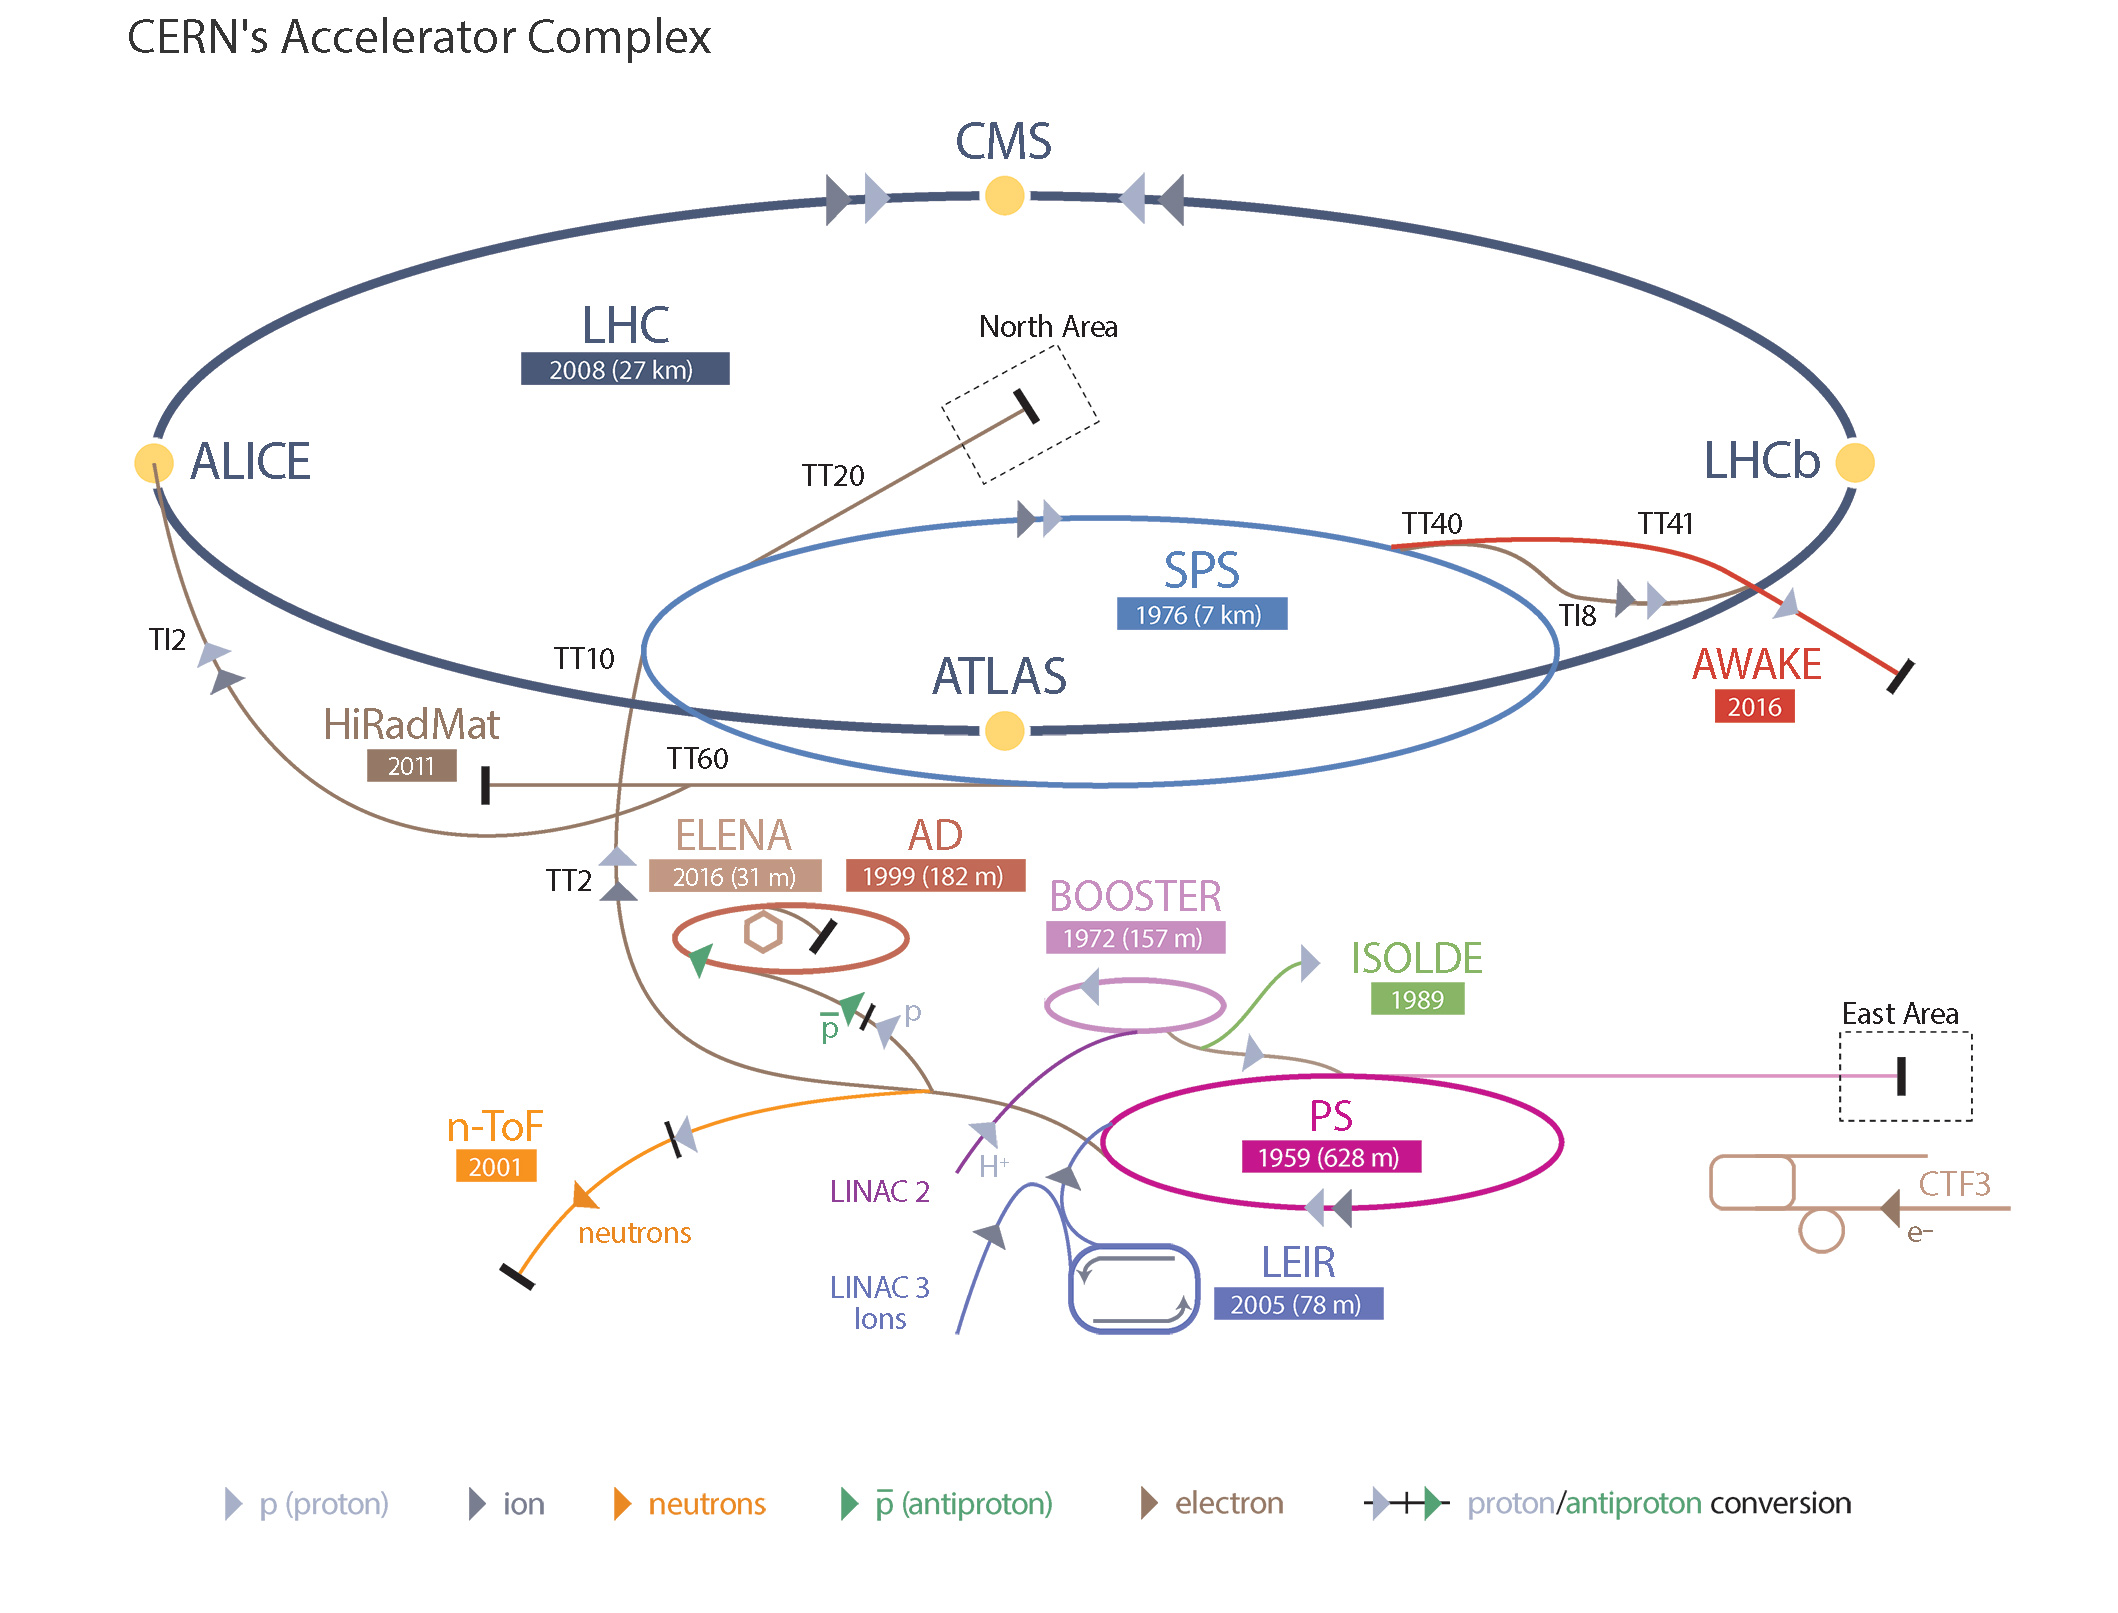
\includegraphics[width=0.8\textwidth]{figures/chapter2/cern_accelerator_complex2}
        \caption{
            Illustration of the various beamlines, accelerator and storage rings, and experimental
            points that the CERN accelerator complex is home to.
            The protons that circulate through the LHC, and that are eventually made to collide inside
            the ATLAS detector, follow the path: Linac 2 $\rightarrow$ Booster $\rightarrow$ Proton Synchotron (PS)
            $\rightarrow$ Super Proton Synchotron (SPS) $\rightarrow$ LHC.
        }
        \label{fig:cern_complex}
    \end{center}
\end{figure}


%%%%%%%%%%%%%%%%%%%%%%%%%%%%%%%%%%%%%%%%%%%%%%%%%%%%%%%%%%%%%%%%%%%
%%%%%%%%%%%%%%%%%%%%%%%%%%%%%%%%%%%%%%%%%%%%%%%%%%%%%%%%%%%%%%%%%%%
% sub-section describing the LHC
%%%%%%%%%%%%%%%%%%%%%%%%%%%%%%%%%%%%%%%%%%%%%%%%%%%%%%%%%%%%%%%%%%%
%%%%%%%%%%%%%%%%%%%%%%%%%%%%%%%%%%%%%%%%%%%%%%%%%%%%%%%%%%%%%%%%%%%
\section{The Large Hadron Collider}
\label{sec:lhc}

The LHC~\cite{LHCMachine} is a circular particle accelerator, with a 27~kilometer circumference,
located at an average distance of 100 meters beneath the surface of the Earth.
It is nominally used for proton-proton ($pp$) collisions, wherein two counter-rotating
beams of protons are made to collide head-on at specific interaction points (IP) along the 27~kilometer
ring, but can also be run in heavy-ion configurations wherein proton-lead ($p$-Pb) or lead-lead (Pb-Pb)
collisions take place.\footnote{The specific lead (Pb) species used in collisions is $^{208}_{82}$Pb.}\footnote{More rarely, the LHC can also be used to circulate gold (Au) ions.
There are even plans to have proton-oxygen ($p$-O) runs in the future, which will allow
for the LHC experiments to provide research that potentially complements dark matter research
based on cosmic-ray air showers.}
The $pp$ collisions take priority over those of the heavy-ions, with the collisions each year
consisting of only a few weeks in the winter for the heavy-ion configurations and typically
six to seven months for the $pp$ configuration. The LHC is designed to accelerate protons to a
center-of-mass energy of $\sqrt{s} = 14\,\TeV$.

\subsection{Machine Design and Layout}
\label{sec:lhc_layout}

\paragraph{Machine Composition} \mbox{} \\
\label{sec:dipole}
The LHC was planned as the successor to the Large Electron Positron (LEP) collider~\cite{LEPI,LEPII}, which was in operation
between the years of 1989 to 2000. LEP is still the most powerful lepton collider to date, having maximal electron-positron
center-of-mass collision energies of 209\,\GeV.
After LEP, the particle physics community knew that the next collider at CERN needed to have $\mathcal{O}(10)$\,\TeV~collision
energies; either to be able to probe from all angles any new physics discovered at LEP and/or the Tevatron~\cite{TevatronDesignI}, or
to provide the necessary power to search for still-elusive hints of BSM physics. At the very least,
given a non-discovery of the Higgs boson at LEP and the Tevatron, the community would need a discovery machine powerful enough
to produce electroweak-scale Higgs bosons and an $\mathcal{O}(10)$ \TeV~hadron collider --- as we now know --- is sufficient for this job.


In order to increase center-of-mass collisions energies, collider designs can take two routes: they can
either increase in size, that is, have larger circumferences (radii), or they can increase the strength of the magnetic
fields used to keep the circulating charged particles in orbit. This can be seen by first considering the expression
for the relativistic cyclotron frequency, $\omega$, of a particle moving in a circular orbit,
\begin{align}
    \omega = \frac{qB}{\gamma m},
    \label{eq:rel_cyclotron}
\end{align}
where $m$ is the particle's rest mass, $B$ is the magnitude of the magnetic field experienced by the
particle, $q$ is the particle's electric charge, and $\gamma$ is the relativistic Lorentz factor, $\gamma = \sqrt{1 - \beta^2} = \sqrt{1 - (v/c)^2}$,
with $v$ the particle's velocity and $c$ the speed of light.
Using Eqn.~\ref{eq:rel_cyclotron}, it can be seen that a particle of higher energy confined to a fixed
circular orbit necessarily has a higher angular velocity by relating the particle's angular
velocity to its kinetic energy:
%A particle of higher energy confined
%to a fixed circular orbit necessarily has a higher
%angular velocity, which can be seen by the expression relating the above angular velocity of the particle to its kinetic energy:
\begin{align}
    E_{\text{kin}} \propto m v^2 = m(\omega R)^2 = \frac{q^2 B^2 R^2}{m \gamma^2}.
    \label{eq:kinetic_energy_gen}
\end{align}
In planning the construction of the LHC, the costs in civil engineering and real-estate works that would
be required to construct a larger tunnel in which to house the LHC ring (increasing $R$) far outweighed
the costs of research into and development of magnet systems strong enough to bend the
multi-\TeV~particles along the beam orbit prescribed by the already-existing LEP tunnel (increasing $B$).
The desired center-of-mass collision energy of $\mathcal{O}(10)$\,\TeV, the fact that the LHC would be a hadron (proton)
collider, and the fact that the LHC would be using the existing LEP tunnel dictate the required magnetic
field strength needed to keep the protons in stable orbits at the LHC. This
is seen by using Eqn.~\ref{eq:kinetic_energy_gen}, solving for $B$, and comparing the LHC and LEP
design parameters,
\begin{align}
    \hspace{-0.4cm}
    \frac{B^2_{\text{LHC}}}{B^2_\text{LEP}} &= \frac{ (E_{\text{LHC}} m_{\text{LHC}} \gamma_{\text{LHC}}^2) / (q_{\text{LHC}}^2 R_{\text{LHC}}^2)  } { (E_{\text{LEP}} m_{\text{LEP}} \gamma_{\text{LEP}}^2) / (q_{\text{LEP}}^2 R_{\text{LEP}}^2) } \label{eq:lhc_mag_field} \\
        &= (E_{\text{LHC}} / E_{\text{LEP}}) \times (m_{\text{LHC}} / m_{\text{LEP}}) \times (\gamma_{\text{LHC}}^2 / \gamma_{\text{LEP}}^2) \times (q_{\text{LEP}}^2 / q_{\text{LHC}}^2) \times (R_{\text{LEP}}^2 / R_{\text{LHC}}^2) \notag \\
        &\approx ( 1\,\TeV~/0.2\,\TeV) \times (m_p/ m_e) \times (1) \times (1) \times (1) \notag \\
        &\approx 10^4 \notag,
\end{align}
which shows that the strength of the LHC bending magnets must be on the order of $100\times$
the strength of those used at LEP. The magnetic fields experienced by the electron and positron beams
at LEP were 0.22 Tesla. By Eqn.~\ref{eq:lhc_mag_field}, the LHC bending magnets should achieve magnetic field
strengths on the order of 10 Tesla in order to achieve the desired collision energies.
The maximum achievable magnetic field of conventional ferrormagnets is about 2 Tesla.
To meet the $\sqrt{s}\approx$10\,\TeV~design goal, the magnet system used by the LHC to confine the protons to their circular orbits
must then be composed of \textit{superconducting} electromagnets. %\footnote{Note that even though
%the main dipole bending magnets at LEP were not superconducting, its focusing quadrupole magnets
%\textit{were} superconducting. There are simply fewer quadrupole magnets, as compared to the number of
%dipole magnets, required for a particle collider.}
The entire magnet system of LEP was therefore removed and replaced with superconducting
niobium-titanium (Nb-Ti) alloy based electromagnets which are superconducting
at temperatures below $10$\,K.
%All of the magnets at the LHC are constructed with
%current carrying elements composed of a niobium-titanium (Nb-Ti) alloy that becomes superconducting
%for temperatures below $10$\,K.
To reach temperatures below this $10$\,K threshold, the LHC magnets
are housed in cryostats that allow for the Nb-Ti elements to be fully submerged in a bath
of superfluid Helium at a temperature of $1.9$\,K~\cite{Casas:1992nf}.
In total, the LHC contains more than 120 tonnes of superfluid Helium.
It goes without saying that there is a significant amount of resources and person power at CERN devoted to the refrigeration and cryogenics
systems that are required for the LHC to run.

Additionally, the fact that LEP was a \textit{particle-antiparticle} collider meant that the counter-rotating
beams could be made to occupy a single ring: the same magnetic field could produce counter-rotating beams of
electrons and positrons within the same beam pipe.\footnote{The electrons and positrons at LEP were vertically separated
within the beam pipe by electrostatic separators placed throughout the LEP ring. Turning off these separators
is, to first approximation, how the LEP operators would get the electrically-attracting electrons and positrons to collide.}
As a result, the LEP beam tunnel was constructed with only a single ring in mind and is relatively narrow: the LEP tunnel,
and therefore LHC tunnel, is only $\approx$3.7\,m wide on average.
As the LHC is a \textit{particle-particle} collider, it necessarily requires \textit{two} magnetic fields
of opposing polarity to circulate one of its beams in the clockwise direction and the other in the
counter-clockwise direction.
Given the limited space in the tunnel, however, it is not possible to house two separate rings
of superconducting bending magnets with all of the services that they require \textit{in addition} to the requisite
minimal space needed for personnel and maintenence access.
This forced the need of the so-called `2-in-1' design of the main bending magnets of the LHC, wherein the two
beam pipes are housed in the same cryostat in which the counter-rotating beams are held in their
respective orbits by coupled magnetic fields.
An illustration of this now-iconic design of the LHC bending (dipole) magnets and surrounding cryostat and containment structure is illustrated in Figure~\ref{fig:lhc_dipole_xsec}.
Each of the 15\,meter long superconducting dipole electromagnets of the LHC responsible for constraining the protons to their circular
orbits has currents of $11850$\,Amperes flowing through it and achieves magnetic field strengths of $8.33$\,Tesla.

\begin{figure}[!htb]
    \begin{center}
        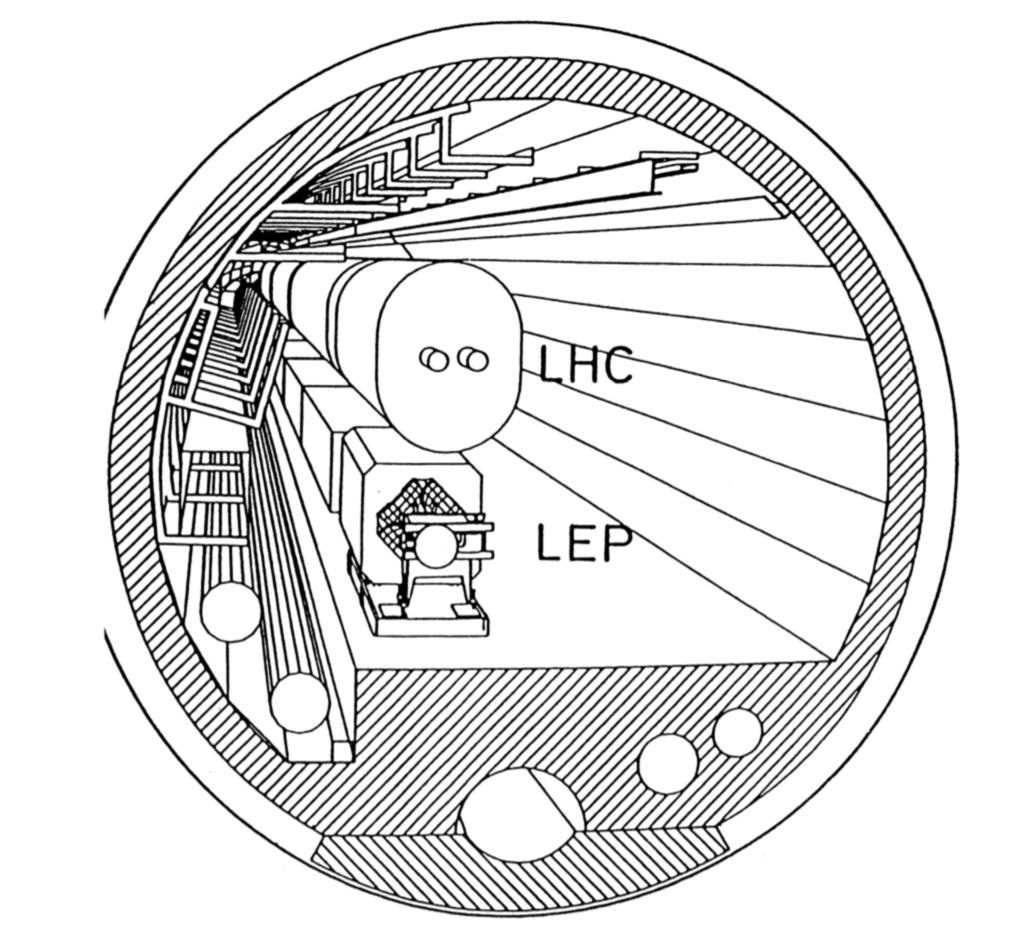
\includegraphics[width=0.43\textwidth]{figures/chapter2/lhc_lep_dipole_comp}
        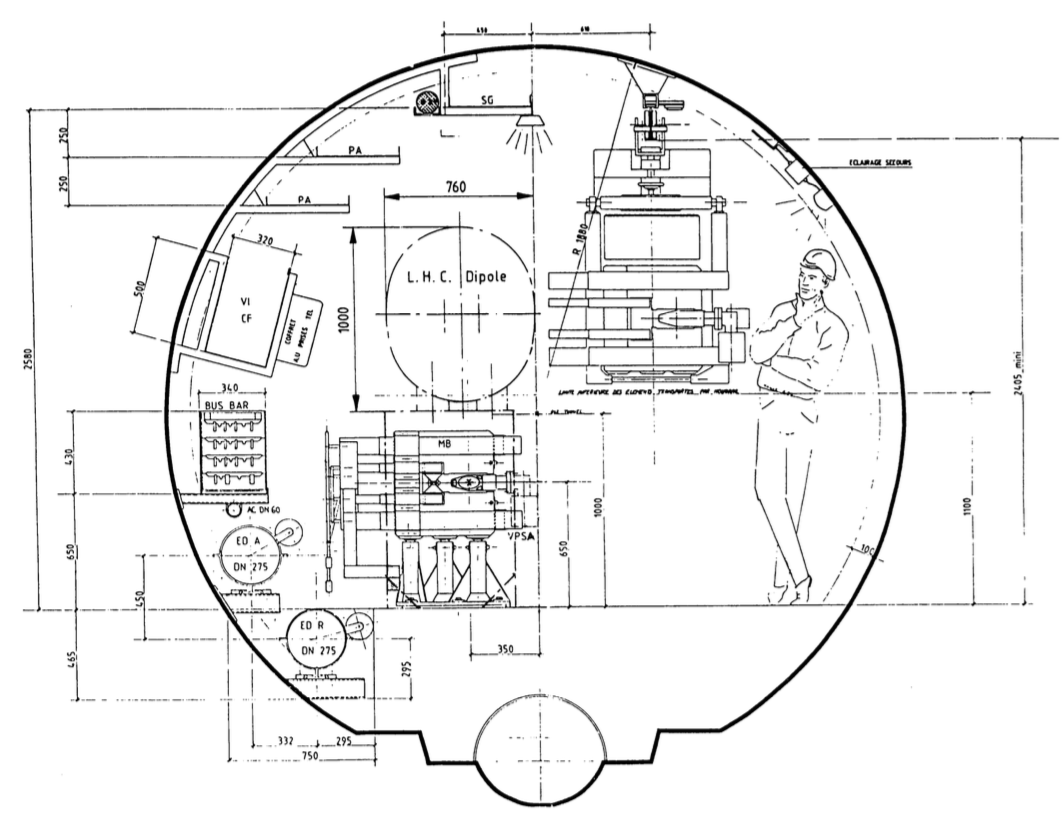
\includegraphics[width=0.50\textwidth]{figures/chapter2/lhc_lep_dipole_comp_person}
        \caption{
            \textit{Left}: Illustration comparing the size of a `2-in-1' LHC dipole configuration to the
                LEP dipole and how they fit inside of the LEP/LHC tunnel. Note that prior to LHC operation,
                the LEP magnets will have been removed: the two are shown side-by-side for comparison purposes only.
            \textit{Right}: Cross-sectional view of the LEP/LHC tunnel with a comparison of the LHC `2-in-1' dipole
                on top of the LEP dipole. An illustration of an average size person is shown
                for scale. Also shown is the service crane in use, to give an idea of the size required
                for potential maintenance access. Clearly, two single-bore, superconducting rings each similar in size
                to the LEP dipole would not fit comfortably in the tunnel. The LHC `2-in-1' design fits
                in nearly the same area as the LEP dipoles while additionally being able to contain both
                particle beams.
                Figures are taken from Ref.~\cite{ECFALHCinLEP}.
        }
        \label{fig:lhc_lep_dipole_comp}
    \end{center}
\end{figure}

\begin{figure}[!htb]
    \begin{center}
        \begin{minipage}{\textwidth}
        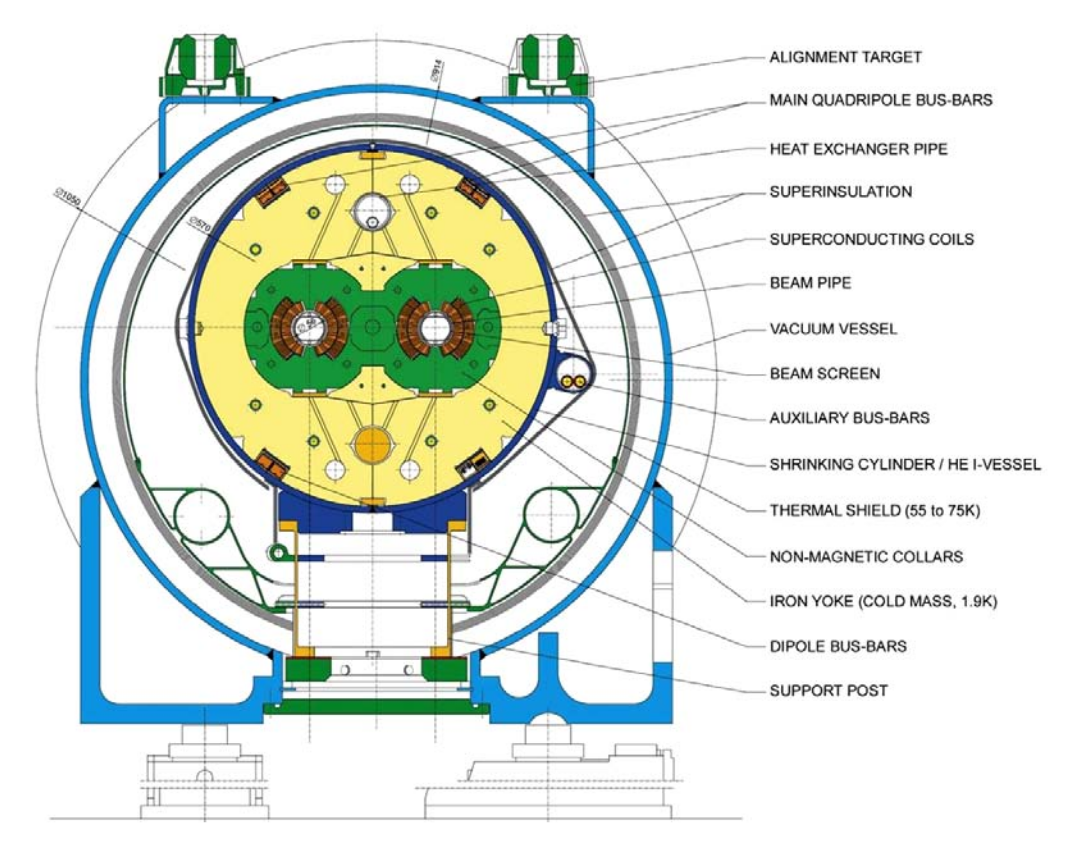
\includegraphics[width=0.59\textwidth]{figures/chapter2/lhc_dipole_fig3p3}
        \raisebox{0.5cm}{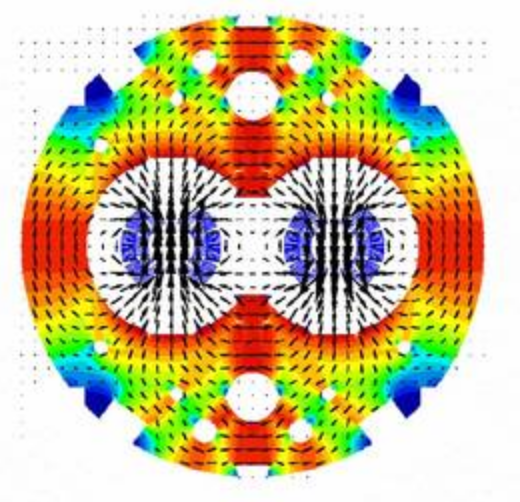
\includegraphics[width=0.4\textwidth]{figures/chapter2/dipole_magnetic_field_lines}}
        \end{minipage}
        \caption{
            \textit{Left}: Cross-sectional view of an LHC dipole bending magnet, with relevant parts indicated.
            The protons orbit inside of the beam pipes, each of which has a diameter of roughly $3$\,cm.
            It is interesting to note that the non-magnetic steel collars (in green) are of critical import
            to the success of the magnet systems. They are required
            to prevent the dipole structure from being deformed or torn apart due to the intense magnetic forces
            tending to push the two beam-pipes apart as a result of their counter-rotating electromagnetic currents.
            These forces amount to about 400 tonnes per meter of dipole when in full operation --- almost equivalent in magnitude
            to the weight of a Boeing 747.
            \textit{Right}: Magnetic field lines of the coupled dipole fields that bend the counter-rotating proton beams
            and keep them in their circular orbits around the LHC ring.
        }
        \label{fig:lhc_dipole_xsec}
    \end{center}
\end{figure}


%\FloatBarrier
\paragraph{Connecting the Dots} \mbox{} \\
The LHC is essentially a chain of superconducting magnets of the type described in the previous paragraphs, where
the the bending (dipole) magnets critical to the LHC design were introduced.
%There are additional
%types of magnets that produce fields of higher multipole moments which, in the case of the quadrupole magnets, are
%necessary for beam \textit{beam focusing}. Conceptually they are very similar to the dipoles and are 
The chain is laid in a double-octagonal structure, illustrated in Figure~\ref{fig:lhc_layout}. There are eight
octants, at the center of which the LHC ring is straight and does not curve.
The LHC curvature occurs at the
boundaries of each of the octants and is primarily made up of bending (dipole) magnets.
The straight sections are where the interaction regions are located and are referred
to as `Points', numbered 1 to 8.
Points 1, 2, 5, and 8 are where the four large LHC experiments are located.
Points 1 and 5 are home to the services and underground areas
of the general purpose experiments, ATLAS and CMS, respectively.
The underground experimental caverns associated with Point 1 and 5 were not present for LEP and
had to be constructed after LEP was retired in 2000.
Figure~\ref{fig:p1} provides an illustration of how the surface and underground
areas are situated at Point 1.
Points 2 and 8 host the services and underground areas of the ALICE and LHCb experiments, respectively.
At these Points, Points 1, 2, 5, and 8, the counter-rotating beams are
made to collide. The remaining Points, Points 3, 4, 6, and 7, are host to various beam `services'
necessary for the operation of the LHC.
Point 3 and 7 host the beam betatron and momentum cleaning (`beam collimation') systems, respectively.
Point 4 hosts the superconducting radio-frequency (RF) systems which accelerate the beams to
their nominal collision energies.
Point 6 is the location of the beam-abort system --- the so-called `beam dump' --- where
the LHC beams may be removed very quickly from the LHC ring by using \textit{kicker} magnets~\cite{LHCDesignI}
that divert the beams out of the LHC ring in a safe manner. The beams may be dumped
if the LHC wishes to refill with protons (or heavy-ions) and needs to remove any
remnants of the previous fill, in case of beam instabilities observed in the LHC ring,
or if one of the experiments signals the need for a beam dump (in case of
beam stability or detector issues observed at the associated IP).

\begin{figure}[!htb]
    \begin{center}
        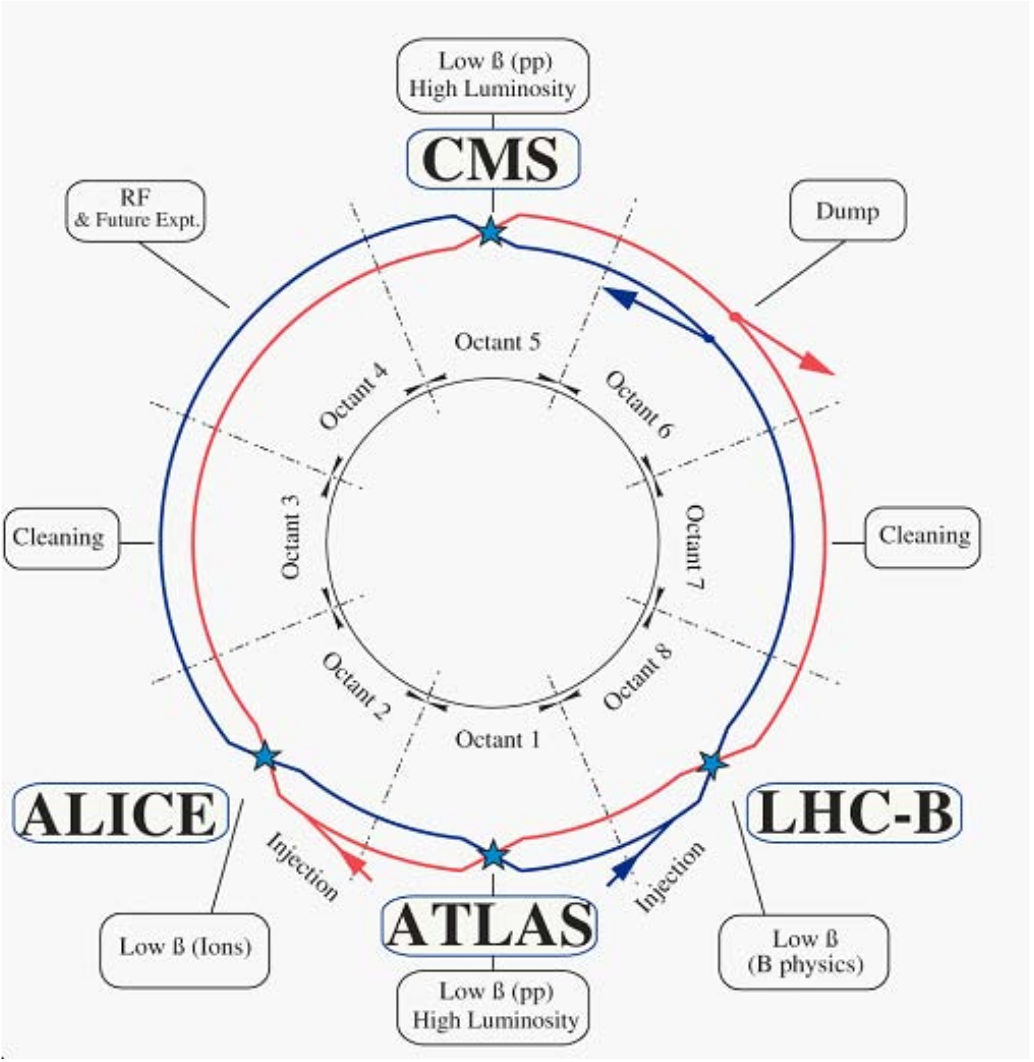
\includegraphics[width=0.8\textwidth]{figures/chapter2/lhc_layout}
        \caption{
            Layout of the LHC and its two counter-rotating beams. Beam 1 is in blue and rotates
            counter-clockwise. Beam 2 is in red and rotates clock-wise.
            At the center of each octant is a straight section which houses
            the experimental caverns or LHC beam facilities.
            At the boundaries of each octant are located the curved sections.
            Figure taken from Figure 2.1 of Ref.~\cite{LHCMachine}.
            {\color{red}{Somewhere $\beta$ should be described -- betatron function}}
        }
        \label{fig:lhc_layout}
    \end{center}
\end{figure}

\begin{figure}[!htb]
    \begin{center}
        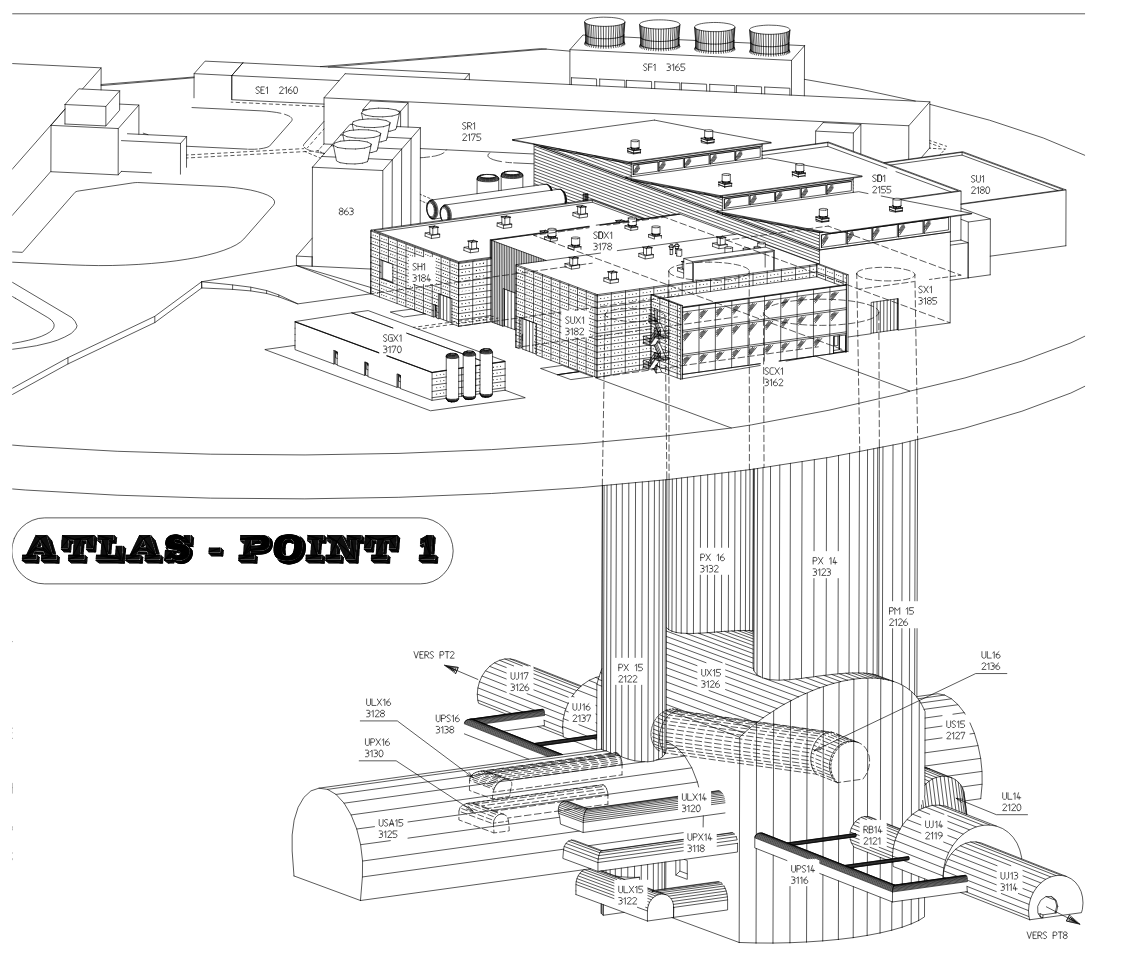
\includegraphics[width=0.75\textwidth]{figures/chapter2/point1_illustration}
        \caption{
            Diagram showing the surface buildings and services and underground areas of Point 1, where
            the ATLAS experiment is located. The LHC ring can be seen at the bottom,
            with its directions indicated by the `VERS PT8 (2)' arrows pointing
            towards Point 8 (2).
            The experimental cavern in which the ATLAS detector sits is UX15.
            The control room for the ATLAS experiment, whereat operators can monitor and
            control the state of the ATLAS detector, is located 100\,m above
            UX15 in the building SCX1.
            Figure taken from Figure 10.1 of Ref.~\cite{LHCDesignII}.
        }
        \label{fig:p1}
    \end{center}
\end{figure}

%\FloatBarrier
\subsection{Injection Chain and Bunch Structure}
\label{sec:lhc_injection}

We now have an idea of how the proton beams relevant to the work
in this thesis are made to circulate in the LHC ring.
In this section we will briefly describe the initial source of the protons and how
they are introduced into the LHC ring.
The LHC relies on a series of pre-acceleration steps that bring the initial
low-energy protons to energies sufficient enough to begin their journey through the LHC.
The sum-total of these steps is referred to as the LHC \textit{injection chain}~\cite{LHCDesignIII}.
The components of the LHC injection chain form the heart of the CERN accelerator
complex illustrated in Figure~\ref{fig:cern_complex}.
For $pp$ collisions in the LHC, the protons are initially sourced from Hydrogen atoms that are released
at the start of Linac 2.
The Hydrogen atoms are immediately stripped of their electrons after passing through
the \textit{duoplasmatron} ion source~\cite{Duoplasma}.
The protons are then passed through Linac 2, a linear accelerator, which accelerates
the protons to $50$\,\MeV.
They then enter the Proton Synchotron Booster (PSB), a circular storage ring
composed of four stacked rings, which accelerates the protons to $1.4\,\GeV$.
The PSB injects the protons into the Proton Synchotron (PS) which accelerates
them to $25$\,\GeV.
The Super Proton Synchotron (SPS) receives the protons from the PS and
accelerates them to $450$\,\GeV.
At this point the protons have sufficient energy to be injected into the LHC.
There are two injection points into the LHC since, up until this stage,
the protons are circulating in the same direction: one injection point sends
protons into the counter-clockwise beamline of the LHC, and the other
into the clockwise beamline.
Until all of the protons from a single \textit{fill} make their way into
the LHC, they will circulate at the injection energy of $450$\,\GeV.
After the filling completes\footnote{A standard LHC fill takes on the order of 4 minutes per
ring.}, the superconducting RF cavities located at Point 4 will begin to accelerate the protons
to their final collision energies.\footnote{If all goes smoothly, this acceleration stage takes roughly 20 minutes.}
The acceleration is achieved by increasing the frequency of the RF oscillations; however,
given that a $450$\,\GeV~proton is already ultra-relativistic, the adjustment of the frequency
needed to get to the collision energies is not large.

The proton beams circulating the LHC are not a continuous stream of protons; rather,
they are grouped into what are referred to as \textit{bunches}.
The protons arrive at the LHC in these bunches which are initially prepared
in the smaller machines that make up the LHC injection chain and then are
kept in their final \textit{bunch structure} by the RF cavities.
The accelerating RF cavities provide an accelerating electromagnetic field
that oscillates longitudinally. The bunches, each composed of roughly $10^{11}$ protons,
are then made to oscillate longitudinally in so-called \textit{synchotron oscillations}
around the central node of the RF oscillation as they circulate through the LHC ring.
The proton bunches are then effectively `shaped' by the oscillating RF field: protons in a bunch
lagging behind or that are ahead of those particles at the center of the bunches
will be accelerated or decelerated accordingly so as to be pushed back into the center of the bunch.
The LHC RF cavities have an oscillation frequency of $400$\,MHz which
defines the boundaries in which proton bunches can lie. These boundaries are
called \textit{RF buckets} and, along with
the circumference of the LHC, dictate the number of proton bunches that
can potentially fit in the LHC.
The relationship between the RF oscillations and the RF bucket and bunch structure
is illustrated in Figure~\ref{fig:lhc_bunch}.
In total, approximately 35640 RF buckets exist when the LHC is in operation.
Not all buckets contain proton bunches, however.
In fact, at the time of the writing of the present thesis,
RF buckets filled with proton bunches have a minimal separation of 10 RF buckets, meaning
that following an RF bucket containing a proton bunch there is at least 9 unfilled RF buckets.
This corresponds to a minimal
time between proton bunches --- the \textit{bunch spacing} --- of $25$\,nanoseconds.
At the time of the present thesis, the operating conditions of the LHC maximally
allow for 2808 $25$\,ns-spaced bunches.\footnote{
The number of allowed bunches is significantly lower than the 35640 RF buckets with $25$\,ns
bunch-spacing potentially allow for. This is due, in part, to the non-trivial bunch-structure
typically employed but also in large part to the fact that there is a rather long \textit{abort gap}
in the LHC ring where no filled RF buckets exist.
The abort gap is a number of continuous unfilled RF buckets that allows the ramp up of the kicker
magnets used for the beam dump to occur in the absence of filled buckets.
In this way, the kicker magnet ramp up does not disturb the structure of the circulating proton beams.
Only after this ramp up is finished should the kicker magnets disturb the beams.
}
The bunch-spacing and overall bunch structure of an LHC fill is not only decided
by the operators of the LHC but also by what the detectors at Points 1,2,5, and 8
can tolerate. This is because shorter bunch spacing means higher intensity and multiplicity
of collisions occuring at each of these IP. A $25$\,nanosecond bunch spacing
corresponds to a maximal $pp$ collision rate of $40$\,MHz. The detectors at each
of the IP have been designed with this collision rate in mind and anything
higher may push them beyond their design limits.

\begin{figure}[!htb]
    \begin{center}
        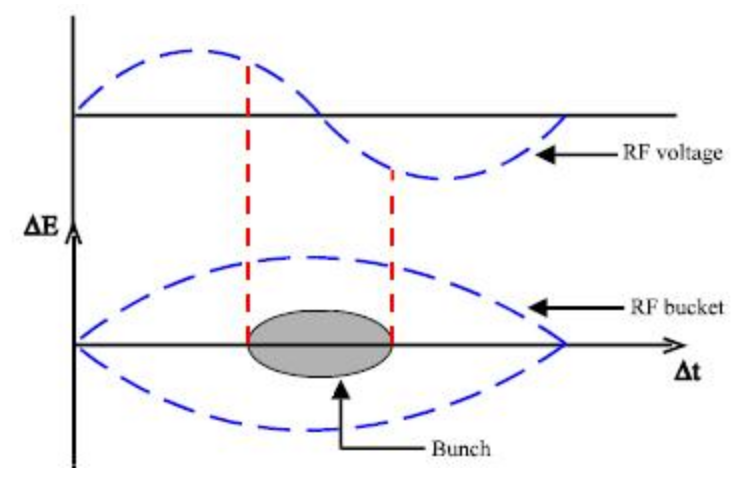
\includegraphics[width=0.5\textwidth]{figures/chapter2/lhc_bunch}
        \caption{
            Illustration of the particle bunch structure in a particle collider such as the LHC.
            The particles are accelerated by radio-frequency (RF) oscillations whose
            amplitude is illustrated in the upper plot.
            The RF bucket's boundary, illustrated in the lower plot, is defined by a full period of the RF oscillation
            and the particle bunch formation, depicted in grey, occurs at the central node of the oscillation.
            The area occupied by the particle bunch is related to the beam's longitudinal
            \textit{emittance}.
        }
        \label{fig:lhc_bunch}
    \end{center}
\end{figure}

\subsection{The Concept of Luminosity}
\label{sec:lhc_luminosity}

In designing a particle collider, the collision energy is not the only important parameter.
Equally important is the value of the instantaneous \textit{luminosity}
that can be achieved by the collider.
An expression for the instantaneous luminosity, $\mathcal{L}$, is given by,
\begin{align}
    \mathcal{L} = \frac{N^2 n_b f}{4 \pi \sigma_x \sigma_y} \cdot S,
    \label{eq:luminosity}
\end{align}
where $N$ is the number of particles per bunch, $n_b$ is the number of colliding bunches,
$f$ is the bunch revolution frequency, $\sigma_{x,y}$ are the transverse beam widths in the
Gaussian approximation, and $S$ is a reduction factor that accounts for geometric factors
such as the non-zero crossing-angle of the colliding beams~\cite{LHCDesignIII,LumiConcept}.
The instantaneous luminosity, $\mathcal{L}$, can be seen by Eqn.~\ref{eq:luminosity}
to have units of cm$^{-2}$s$^{-1}$ and can be conceptually thought of as the
outgoing flux of particles per unit area and time after a bunch crossing in which successful $pp$
collisions occur.
The LHC is designed to deliver collisions to the high luminosity IP (Fig.~\ref{fig:lhc_layout})
at $\mathcal{L} = 10^{34}$\,cm$^{-2}$s$^{-1}$.
Accurate knowledge of $\mathcal{L}$ is of the utmost importance for collider design and operation.
Not only does it parametrise the potential collision rate once the collider beam and bunch
structure are decided, but it allows for the accurate prediction of the number
of collision events, $N_{\text{proc}}$, associated with a particular physics process
with cross-section $\sigma_{\text{proc}}$,
\begin{align}
    N_{\text{proc}} = \sigma_{\text{proc}} \int \mathcal{L}\, \mathrm{d}t \equiv \sigma_{\text{proc}} \cdot L,
    \label{eq:n_exp_lumi}
\end{align}
where $L$ is referred to as the \textit{integrated luminosity} and has units of cm$^{-2}$.
A common unit for integrated luminosity is the \textit{barn}, with symbol `b': one barn is defined as $10^{-24}$\,cm$^{-2}$.
The datasets collected by the LHC experiments are such that the \textit{femtobarn} (fb), $10^{-39}$\,cm$^{-2}$, is relevant.

\subsection{Operation of the Large Hadron Collider}
\label{sec:lhc_operation}

The LHC has been in stable operation since 2009.
It operates in so-called \textit{runs}: multi-year periods of roughly continuous
data-taking.
As CERN shuts down during the winter months, each run is segmented each year
with a several month long shutdown in the winter with a ramp-up period in the spring.
During these shorter shutdowns, maintenance and upgrades may also take place.
In between a given run there is a multi-year break, a \textit{long shutdown},
in which large(er)-scale maintenance and upgrades of both the LHC and the experiments can take place.
At the time of writing, there has so far been two runs of the LHC, Run-I and Run-II.
Run-I took place during the years 2009--2012 and Run-II during 2015--2018.
The integrated luminosities for each of the data taking years between Run-I and Run-II
is shown in Fig.~\ref{fig:int_lumi_multiyear}.
The data relevant to the work presented in this thesis were collected in both
Run-I and Run-II of the LHC, specifically that data collected in the years 2012--2018.
The luminosities, instantaneous and integrated, as well as the center-of-mass collision energies, $\sqrt{s}$, for these data-taking periods are
shown in Table~\ref{tab:lumi_tab}.
Also shown in Table~\ref{tab:lumi_tab} are the average values of the mean number of interactions per bunch
crossing, $\langle \mu \rangle$, observed during each data-taking year. The quantity $\langle \mu \rangle$
is related to the amount of \textit{pileup} observed during data-taking. Pileup is caused
by overlapping $pp$ interactions within the same (\textit{in-time} pileup) or neighboring (\textit{out-of-time} pileup)
bunch-crossing(s) at the interaction point. The pileup scales with the instantaneous luminosity.
Distributions of $\langle \mu \rangle$ are shown in Fig.~\ref{fig:int_lumi_multiyear} for
the Run-II data-taking period.


\begin{table}[!htb]
    \begin{center}
        \begin{tabular}{l | c | c c c c }
        \hline
        \hline
        & \textbf{Run-I} & \multicolumn{4}{c}{\textbf{Run-II}} \\
        \hline
        Year & 2012 & 2015 & 2016 & 2017 & 2018 \\
        \hline
        Collision energy, $\sqrt{s}$ [TeV] & 8 & \multicolumn{4}{c}{13} \\
        Peak Luminosity, $\mathcal{L}$ [cm$^{-2}$s$^{-1}$] ($\times10^{34}$) & $0.77$ & $0.5$ & $1.4$ & $2.1$ & $2.1$ \\ 
        Integrated Luminosity, $L$ [fb$^{-1}$] & 20.2 & 3.2 & 33.0 & 44.3 & 59.9 \\
        Mean number of of interactions & & & & & \\
        \hspace{1.7cm} per bunch crossing, $\langle \mu \rangle$ & 20.7 & 13.4 & 25.1 & 37.8 & 36.1 \\
        \hline
        \hline
        \end{tabular}
        \caption{
            Summary parameters for the data-taking periods relevant to the work
            presented in this thesis. The integrated luminosity is that relevant
            to performing physics analysis and potentially differs with respect to
            the total integrated luminosity delivered to ATLAS by the LHC (Fig.~\ref{fig:int_lumi_multiyear}) due to
            the application of strict quality criteria on the data prior to its use
            in physics analyses.
        }
        \label{tab:lumi_tab}
    \end{center}
\end{table}

\begin{figure}[!htb]
    \begin{center}
        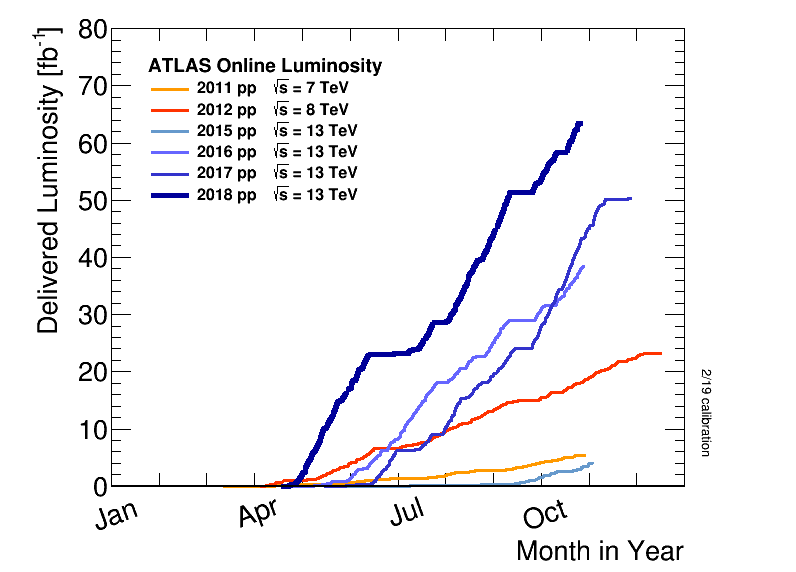
\includegraphics[width=0.49\textwidth]{figures/chapter2/int_lumi_multiyear}
        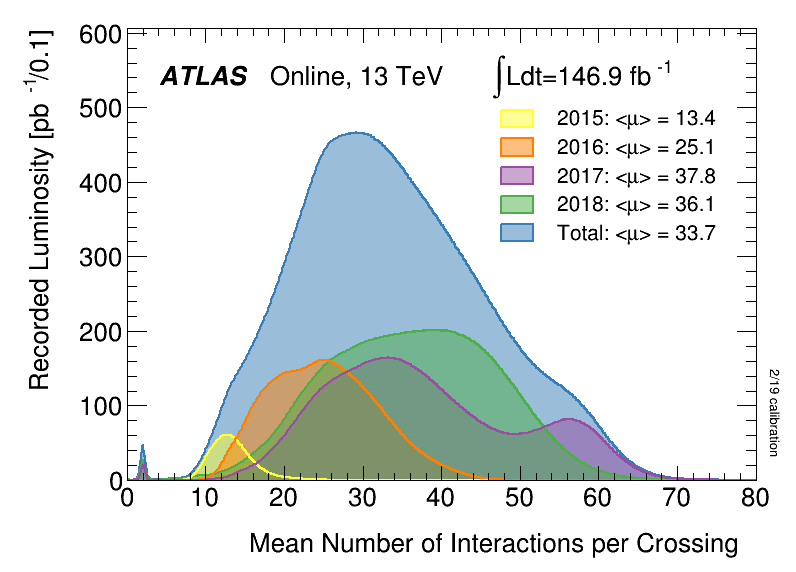
\includegraphics[width=0.49\textwidth]{figures/chapter2/mu_run2}
        \caption{
            \textit{Left}: The ATLAS integrated luminosity during the data-taking years 2011--2018.
            \textit{Right}: The observed average number of $pp$ interactions per bunch-crossing, $\langle \mu \rangle$,
                observed by ATLAS during the Run-II data-taking years, 2015--2018.
        }
        \label{fig:int_lumi_multiyear}
    \end{center}
\end{figure}


%%%%%%%%%%%%%%%%%%%%%%%%%%%%%%%%%%%%%%%%%%%%%%%%%%%%%%%%%%%%%%%%%%%
%%%%%%%%%%%%%%%%%%%%%%%%%%%%%%%%%%%%%%%%%%%%%%%%%%%%%%%%%%%%%%%%%%%
% sub-section describing ATLAS
%%%%%%%%%%%%%%%%%%%%%%%%%%%%%%%%%%%%%%%%%%%%%%%%%%%%%%%%%%%%%%%%%%%
%%%%%%%%%%%%%%%%%%%%%%%%%%%%%%%%%%%%%%%%%%%%%%%%%%%%%%%%%%%%%%%%%%%
\section{The ATLAS Detector}
\label{sec:atlas}

In this section we will extend our focus to the ATLAS detector, the general purpose
particle detector located at Point 1 of the LHC ring (see Figure~\ref{fig:p1}).
Roughly cylindrical in shape, coaxial with the beam-pipe,
the ATLAS detector is 44\,m long and 25\,m tall.
It is by far the largest such detector ever built and,
generally, is the largest and most complex device ever constructed.
Being general purpose in scope, the ATLAS detector is hermetic and has
nearly $4\pi$ radians of solid angle coverage around the $pp$ collision
point. 
Such detectors are commonly designed to have various subsystems --- \textit{subdetectors} ---
which are designed for the identification of specific types of particles
and interactions.
They tend to be layered about the interaction point and cylindrically symmetric
since the $pp$ interactions taking place within the detector have no preferred
direction in the plane transverse to the direction in which the proton beams
are travelling.
A view of the ATLAS detector and its subdectors is provided by Figure~\ref{fig:atlas_cutaway}.
In the following we will briefly describe each subsystem in turn, describing
first the detectors located nearer to the $pp$ collision and proceeding outwards.

\subsection{The ATLAS Coordinate System}
\label{sec:atlas_coordinate_system}

The ATLAS detector uses a right-handed coordinate system with the origin located at
the geometric center of the detector.
The $x$-axis points to the center of the LHC ring, the $y$-axis points upwards
and away from the center of the Earth, and the $z$-axis is along the beam-pipe.
The side associated with positive (negative) $z$
is referred to as the `A' (`C') side of the detector.\footnote{`A' for `airport',
since this is the side pointing towards Geneva International Airport, and
`C' for either `Crozet' or `Charly's', depending on who you ask, since this is the side
pointing towards the town of Crozet and/or Charly's Pub in the town of Saint-Genis-Pouilly.}
Due to its cylindrical symmetry, ATLAS also uses the cylindrical coordinates, $(r,\phi, z)$,
with $\phi$ the azimuthal angle about the $z$-axis and having $\phi = 0$ along the positve $x$-axis.
The spherical polar angle, $\theta$, is defined with respect to the $z$-axis, having
$\theta = 0$ parallel to the beam-pipe and $\theta = \pi/2$ in the $xy$-plane transverse
to the beam-pipe.
The pseudorapidity, $\eta$, is commonly used when describing systems of particles or locations within
the detector and is defined as $\eta = - \ln \left[ \tan \left( \theta / 2 \right) \right ]$.
The relationship between pseudorapidity and polar angle is illustrated in Figure~\ref{fig:eta_desc}.
Large (small) values of $\eta$ correspond to the \textit{forward} (\textit{central}) region of the detector.
The rapidity, $y$, is related to $\eta$ and is defined as $y = \frac{1}{2} \ln \left[ (E+p_z) / (E-p_z) \right]$.
The pseudorapidity of a particle traversing the detector is equal to its rapidity if
the particle is massless or ultra-relativistic; otherwise, they are different.
The comparison between a particle's pseudorapidity and rapidity is illustrated in
Figure~\ref{fig:eta_desc}.
The coordinates used to describe systems of particles are typically described by their
four-momenta: $(p_x, p_y, p_z)$ or, equivalently, $(\pT, \eta, \phi)$.
A distance metric commonly used to describe the distance between two systems of particles
in the detector is $\Delta R = \sqrt{ (\Delta \eta)^2 + (\Delta \phi)^2 }$. The
$\Delta R$ quantity using $y$ instead of $\eta$ is also sometimes used and will be
indicated by $\Delta R_y$.

\begin{figure}[!htb]
    \begin{center}
        \raisebox{1.5cm}{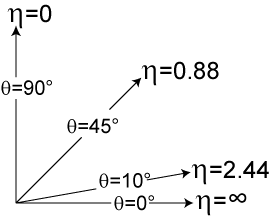
\includegraphics[width=0.35\textwidth]{figures/chapter2/eta_vs_polar}}
        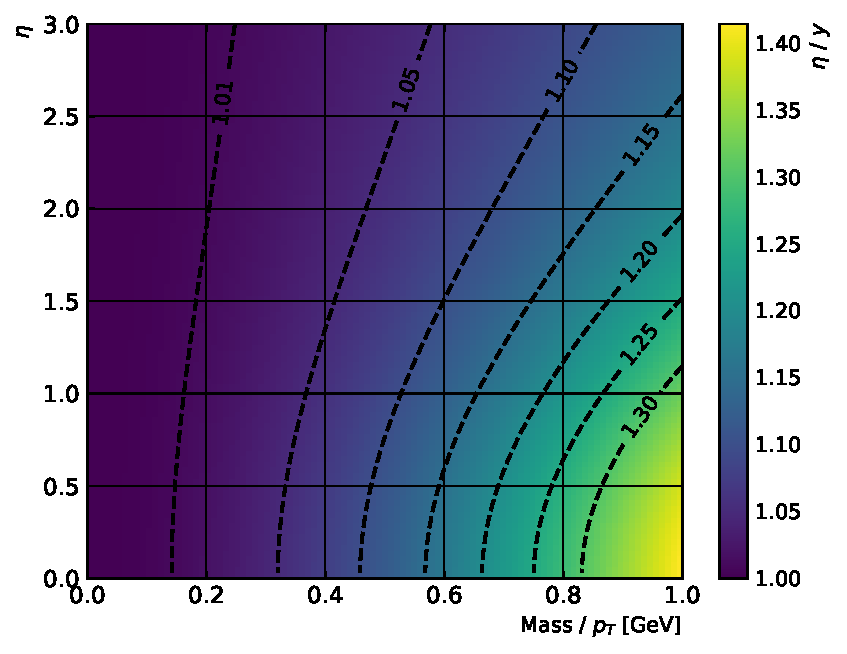
\includegraphics[width=0.55\textwidth]{figures/chapter2/eta_vs_rap}
        \caption{
            \textit{Left}: Illustration of the relationship between the pseudorapidity, $\eta$,
                and polar angle, $\theta$, defined as the angle with respect to the beam-axis ($z$-axis).
            \textit{Right}: Distribution of the ratio of a particle's pseudorapidity to its rapidity, $\eta$/$y$,
                as a function of its pseudorapidity ($y$-axis) and the ratio of its mass to its transverse momentum, \pT~($x$-axis).
        }
        \label{fig:eta_desc}
    \end{center}
\end{figure}


\begin{figure}[!htb]
    \begin{center}
        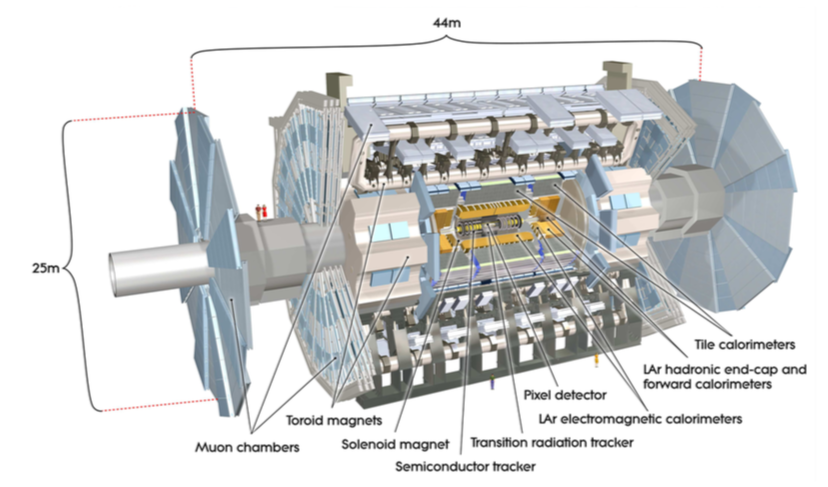
\includegraphics[width=0.95\textwidth]{figures/chapter2/atlas_cutaway}
        \caption{
            Cut-away view of the ATLAS detector with sub-systems indicated.
            Shown for comparison are figures of average-height humans standing
            at the feet of the detector and standing on the forward shielding
            between the big wheels of the forward muon system.
        }
        \label{fig:atlas_cutaway}
    \end{center}
\end{figure}


\begin{figure}[!htb]
    \begin{center}
        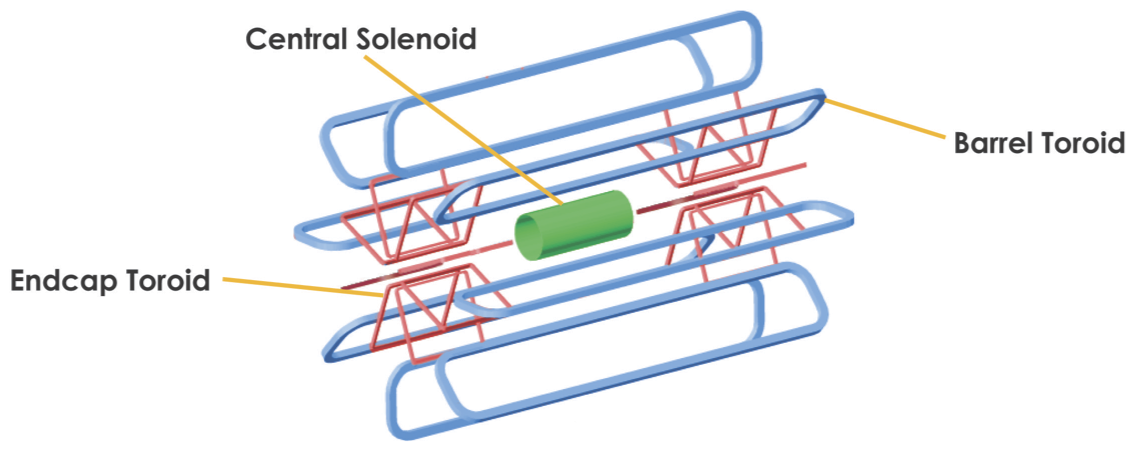
\includegraphics[width=0.95\textwidth]{figures/chapter2/atlas_magnet_system}
        \caption{
            A view of the ATLAS magnet system. Shown are the 2\,T solenoid magnet
            in green, the barrel toroid system in blue, and endcap toroid magnets
            in red.
        }
        \label{fig:atlas_magnet_system}
    \end{center}
\end{figure}

%%%%%%%%%%%%%%%%%%%%%%%%%%%%%%%%%%%%%%%%%%%%%%%%%%%%%%%%%%%%%%%%%%%%%
%%%%%%%%%%%%%%%%%%%%%%%%%%%%%%%%%%%%%%%%%%%%%%%%%%%%%%%%%%%%%%%%%%%%%
%
% INNER DETECTOR
%
%%%%%%%%%%%%%%%%%%%%%%%%%%%%%%%%%%%%%%%%%%%%%%%%%%%%%%%%%%%%%%%%%%%%%
%%%%%%%%%%%%%%%%%%%%%%%%%%%%%%%%%%%%%%%%%%%%%%%%%%%%%%%%%%%%%%%%%%%%%
\subsection{The Inner Detector}
\label{sec:inner_detector}

The innermost subdetector of ATLAS is the Inner Detector (ID)~\cite{Haywood:331064}.
The ID covers the region $\lvert \eta \rvert < 2.5$ and is composed, in order
of increasing radial distance from the beam-pipe, of the pixel detector,
semiconductor tracker (SCT), and the transition radiation tracker (TRT).
These detectors enable the reconstruction of the tracks associated with
the $\mathcal{O}(1000)$ charged particles emerging from each $pp$ bunch collision, occuring
every 25\,ns.
An illustration of the ID and its subdetectors is shown in Figure~\ref{fig:atlas_inner_detector}.
Additional, more detailed views of the barrel and endcap sections of the ID are shown in Figure~\ref{fig:atlas_ID_exploded}.
The ID is situated inside of the central solenoid, indicated in Figure~\ref{fig:atlas_magnet_system},
which provides an axial 2\,T magnetic field and extends over a length of 5.3\,m with a diameter of 2.5\,m.
The bending of charged particles in the $xy$-plane due to the presence of the solenoidal
field allows for their momenta to be measured using the curvature of their reconstructed tracks.

\begin{figure}[!htb]
    \begin{center}
        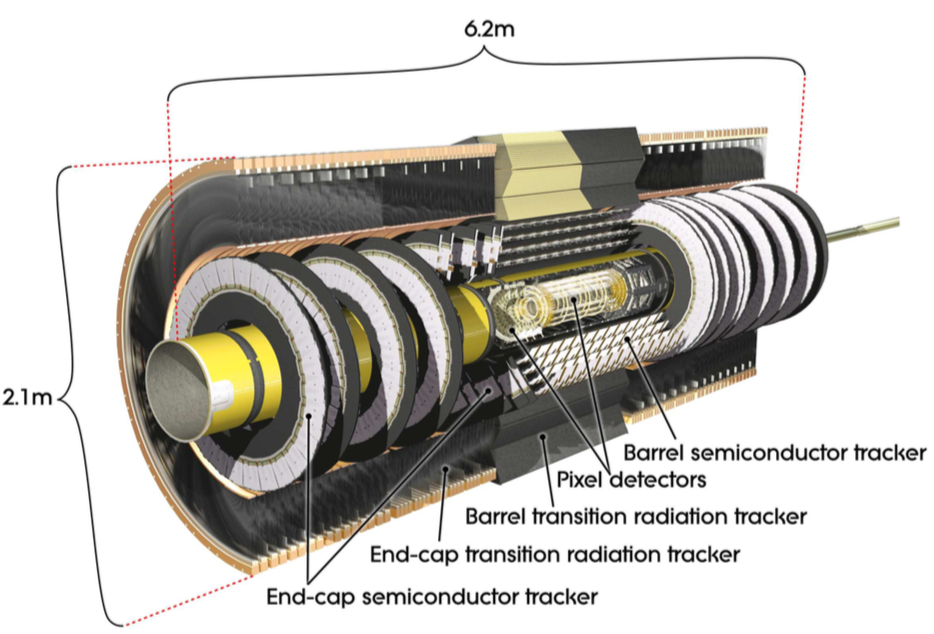
\includegraphics[width=0.75\textwidth]{figures/chapter2/atlas_inner_detector}
        \caption{
            Cross-sectional view of the ATLAS inner detector. Shown are the barrel
            and end-cap portions of the pixel, SCT, and TRT detectors.
        }
        \label{fig:atlas_inner_detector}
    \end{center}
\end{figure}

\begin{figure}[!htb]
    \begin{center}
        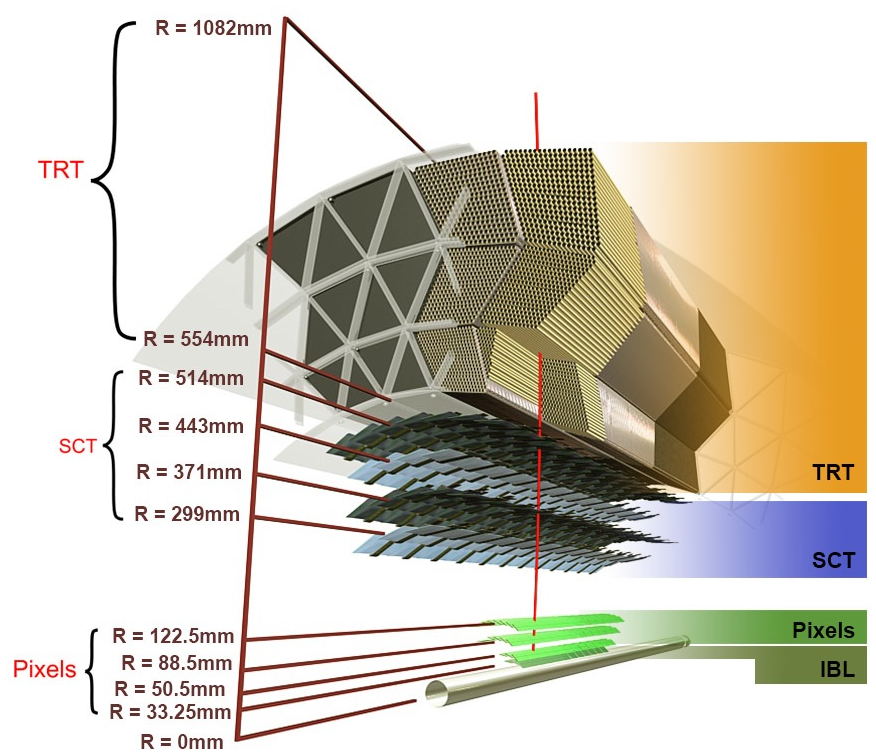
\includegraphics[width=0.6\textwidth]{figures/chapter2/atlas_ID_barrel_exploded}
        \raisebox{1.4cm}{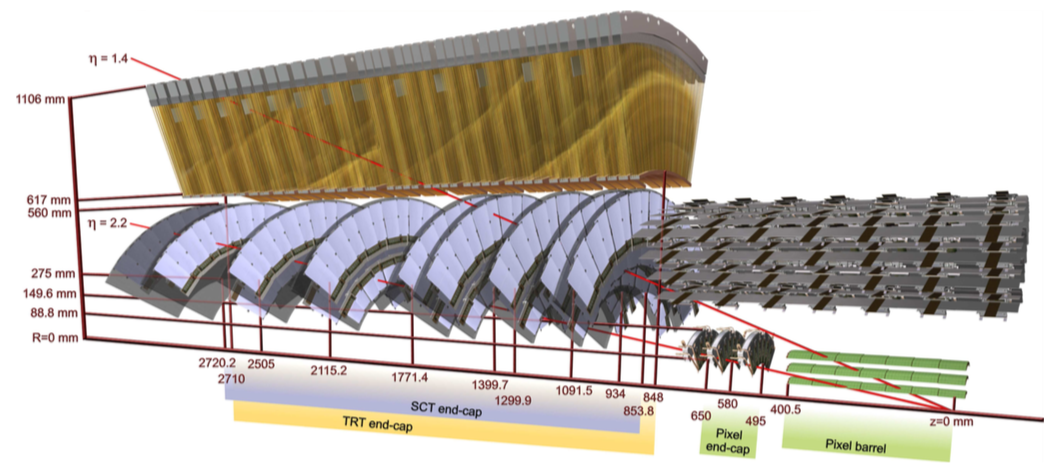
\includegraphics[width=0.85\textwidth]{figures/chapter2/endcap_ID_exploded}}
        \caption{
            Exploded views of the barrel (\textit{left}) and endcap (\textit{right}) portions
            of the inner-detector.
        }
        \label{fig:atlas_ID_exploded}
    \end{center}
\end{figure}

\subsubsection{The Pixel Detector and IBL}
\label{sec:id_pixel}

The pixel detector is the innermost subdetector of the ID, situated very near to and surrounding
the beam-pipe.
It is composed of three separate sections: a barrel section and two end-cap sections.
The barrel section  of the pixel detector has a cylindrical geometry and the end-cap sections
are disks centered on the beam-pipe.
The barrel section has four layers, each with increasing radius, and there are three disks in each
of the end-caps. This ID geometry, shown in Figure~\ref{fig:atlas_ID_exploded}, covers
the region $\lvert \eta \rvert < 2.5$.

The pixel detector, being so near the $pp$ collisions, is subject to the highest particle
fluxes of any other subsystem.
As a result, it is built to have very fine granularity: its sensing elements consist of
$250$\,\micron~thick detectors housing pixels of reverse-biased n-type semiconductor material,
each having a nominal size of $50\times400\,\micron^2$.
In total, there are roughly 80 million channels read out from the pixel detector alone.
This allows for the pixel detector's fine spatial hit resolution of $10\,\micron$ in
$(r-\phi)$ and $115\,\micron$ along $z$.

The innermost layer of the pixel detector's barrel section is referred to as the
\textit{Insertable B-Layer} (IBL), and was installed at the beginning of the Run-II
data-taking period~\cite{Capeans:1291633}.
It corresponds, essentially, to the instrumentation of the ATLAS beam-pipe, as seen in Figure~\ref{fig:pixel_detector_trans},
and is located at a radial distance of 3.3\,cm.
It alone accounts for 8 million readout channels of
the pixel detector --- resulting in an ultra precise spatial hit resolution of $8\,\micron$ in $(r-\phi)$ and
$40\,\micron$ along $z$.
Beyond improving the overall measurements and reconstruction of charged particle tracks,
the IBL was installed in order to improve the performance of secondary vertex
reconstruction --- an essential ingredient to the algorithms associated with
the reconstruction and identification of jets originating from the decays
of $b$-hadrons whose decays occur at radial distances frequently beyond that
of the IBL.



\begin{figure}[!htb]
    \begin{center}
        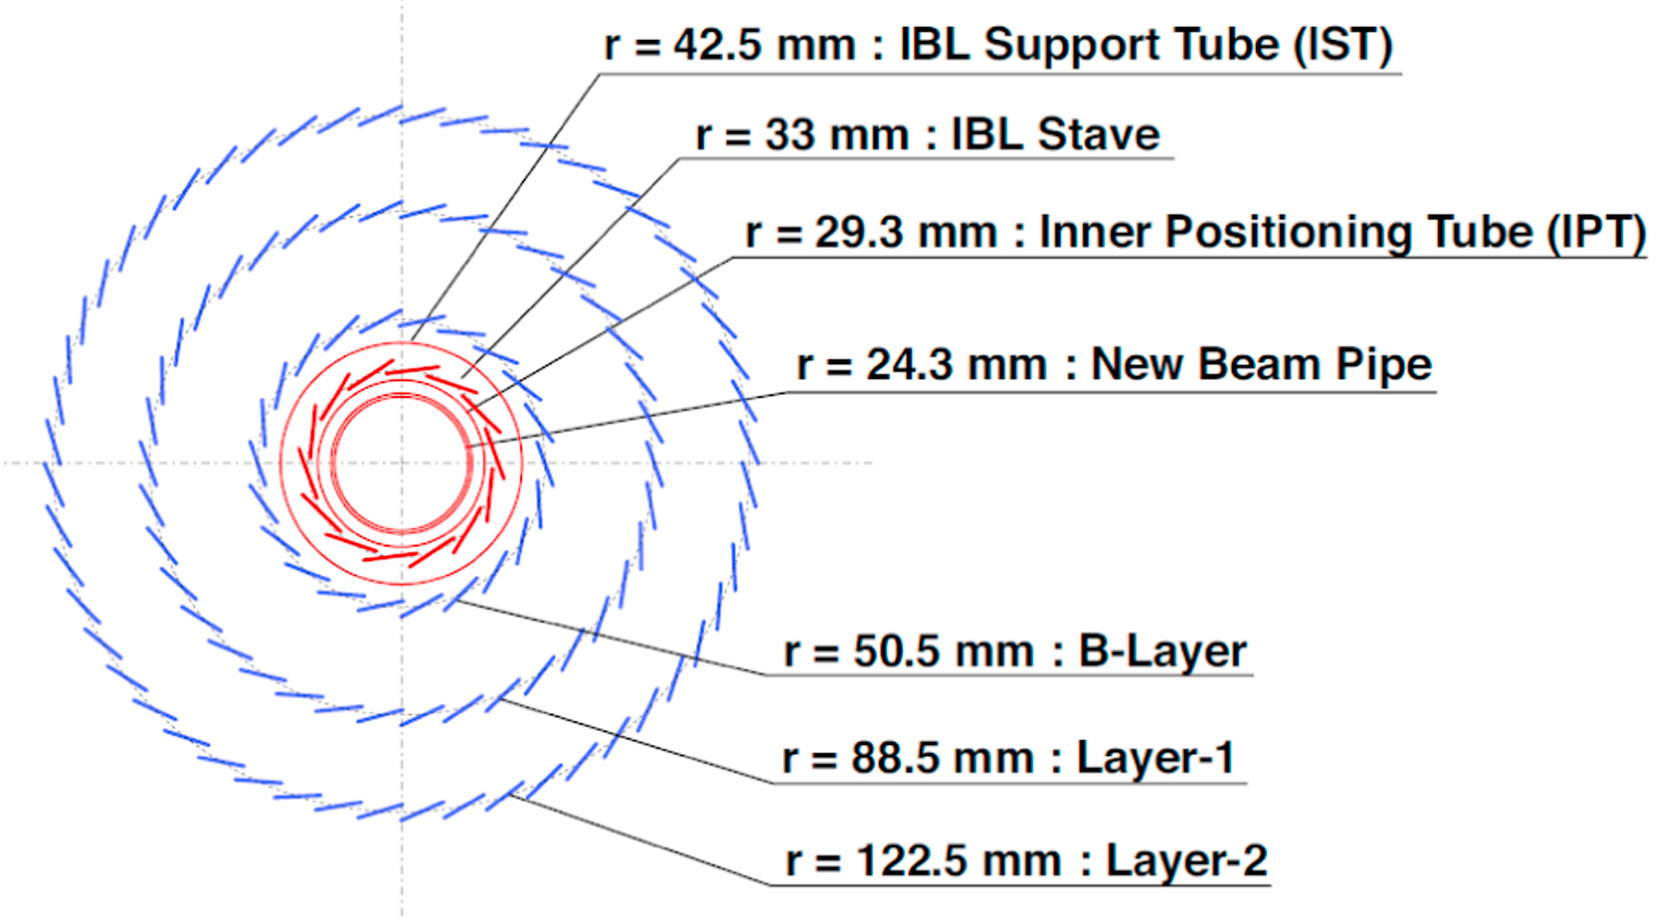
\includegraphics[width=0.8\textwidth]{figures/chapter2/pixel_detector_trans}
        \caption{
            Transverse view of the barrel section of the pixel detector, showing
            the innermost layer, the Insertable B-Layer (IBL) (red), and the
            three surrounding layers (blue). From Ref.~\cite{Backhaus:2016ctq}.
        }
        \label{fig:pixel_detector_trans}
    \end{center}
\end{figure}


%%%%%%%%%%%%%%%%%%%%%%%%%%%%%%%%%%%%%%%%%%%%%%%%%%%%%%%%%%%%%%%%%%%%%
%%%%%%%%%%%%%%%%%%%%%%%%%%%%%%%%%%%%%%%%%%%%%%%%%%%%%%%%%%%%%%%%%%%%%
%
% CALORIMETERS
%
%%%%%%%%%%%%%%%%%%%%%%%%%%%%%%%%%%%%%%%%%%%%%%%%%%%%%%%%%%%%%%%%%%%%%
%%%%%%%%%%%%%%%%%%%%%%%%%%%%%%%%%%%%%%%%%%%%%%%%%%%%%%%%%%%%%%%%%%%%%
\subsection{Calorimeter Systems}
\label{sec:calorimeters}

The ATLAS calorimeter systems are situated outside of the ID and central solenoid and
are tasked with the measurement and containment of showers from electrically charged and neutral particles.
A view of the calorimeter systems is provided by Figure~\ref{fig:atlas_calorimeters_cutaway}.
Broadly speaking, there are two types of calorimeters based on their purpose:
electromagnetic and hadronic calorimeters.
The electromagnetic calorimeter system has $\eta$ coverage that matches the inner-detector
and is optimized for precision measurements of electrons and photons.
The hadronic calorimeter system has readout cells that are generally of
coarser granularity as compared to the electrogmagnetic calorimeter and
is designed to meet the requirements for jet and missing transverse momentum
measurements.
Besides classification by physics purpose, the calorimeter system can also
be broken into two classes based on detector technology: either based
on gaps of cooled liquid-argon~\cite{CERN-LHCC-96-041} or on scintillating tiles as the active media~\cite{CERN-LHCC-96-042}.

\begin{figure}[!htb]
    \begin{center}
        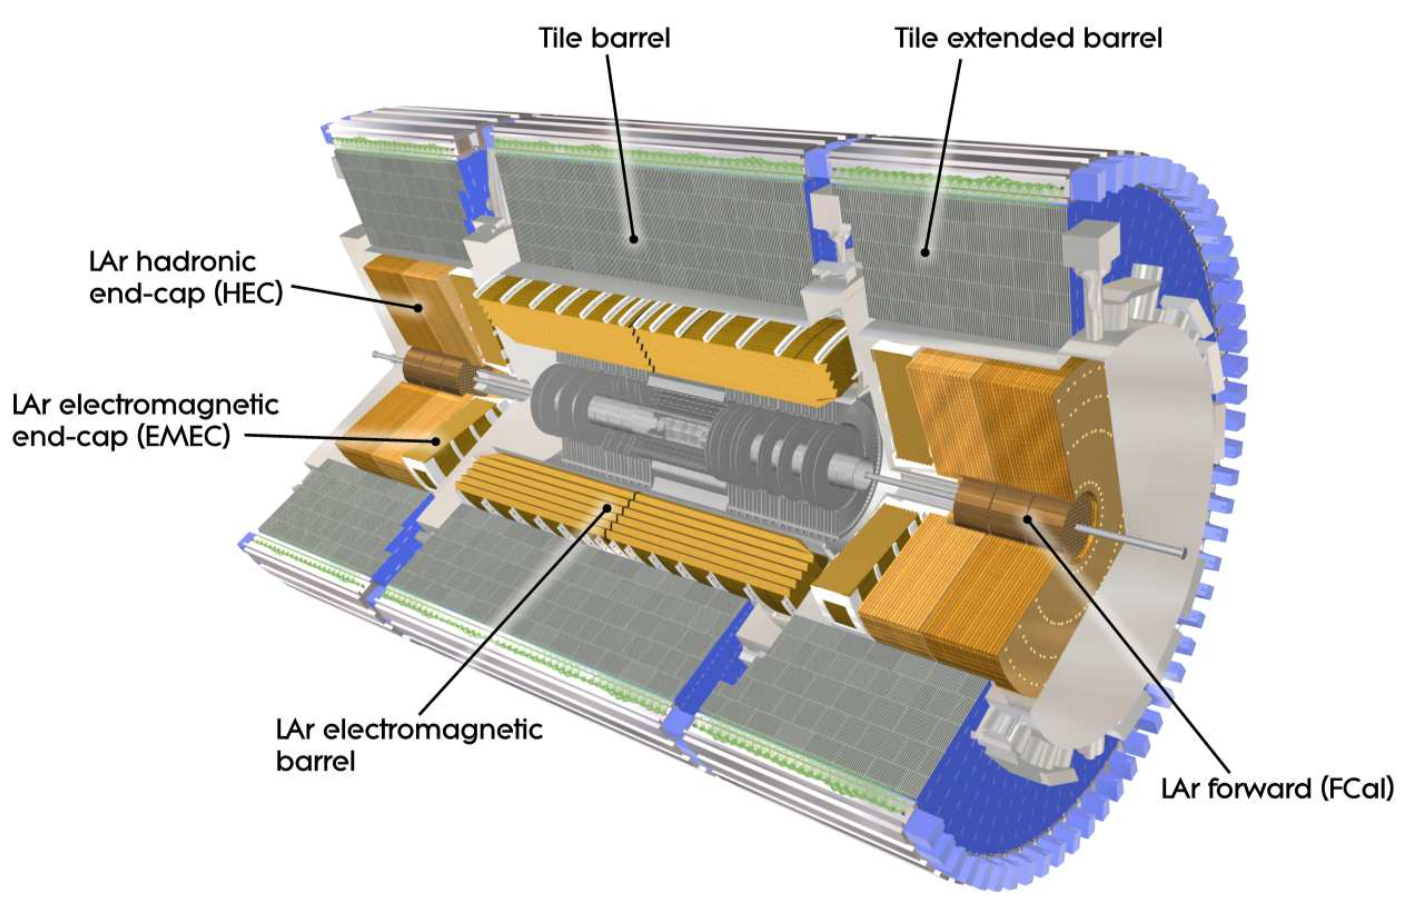
\includegraphics[width=0.9\textwidth]{figures/chapter2/calorimeters/atlas_calorimeter_cutaway}
        \caption{
            Cut-away view of the ATLAS calorimeter system, with liquid-argon and sctintillating-tile
            subsystems indicated.
        }
        \label{fig:atlas_calorimeters_cutaway}
    \end{center}
\end{figure}

\subsubsection{Electromagnetic Calorimeter}
\label{sec:calo_em}

The electromagnetic (EM) calorimeter is a high-granularity lead/liquid-argon (LAr)
sampling calorimeter situated outside of the ID and sharing the
same cryostat as the the central solenoid.
It consists of barrel and end-cap sections that cover the entire
range within $\lvert \eta \rvert < 3.2$ and is illustrated in Figure~\ref{fig:atlas_calorimeters_cutaway}.
The structures of the electromagnetic barrel and end-cap calorimeters
are shown in Figure~\ref{fig:em_calo_section}.
The EM calorimeter is designed in an accordian type structure to provide full coverage
in $\phi$.
The cooled LAr fills the gaps between layers of the
accordian structure.
Passing particles from the interaction point undergo scattering and bremsstrahlung processes as they pass through
the lead absorbers. The resulting electrons and photons ionise the LAr, producing
drift electrons and ions whose signals are read out by the interleaved readout
electrodes. The 2.1\,mm drift gap has an operating voltage of $\approx 2$\,kV.
The electromagnetic calorimeter is $>22$ radiation lengths ($X_0$), ensuring
that the majority of electrons and photons are completely contained within the EM calorimeter.
The majority of the EM energy, amounting to approximately 16\,$X_0$, is contained
within the second sampling layer (see Figure~\ref{fig:em_calo_section}).
The fine granularity of the readout, indicated in Figure~\ref{fig:em_calo_section},
was designed with the ability to distinguish individual photons arising from $\pi^0 \rightarrow \gamma \gamma$
decays. The ability to distinguish photons pairs so precisely is also important for the
main Higgs boson decay channel used for its disovery, $h \rightarrow \gamma \gamma$.

In the region $\lvert \eta \rvert < 1.8$, a so-called \textit{presampler} detector is used to correct
for the energy lost by electrons and photons due to material interactions occuring
upstream of the EM calorimeter.
It is a single LAr layer, with width 1.1\,cm (0.5\,cm) in the barrel (end-cap).

\begin{figure}[!htb]
    \begin{center}
        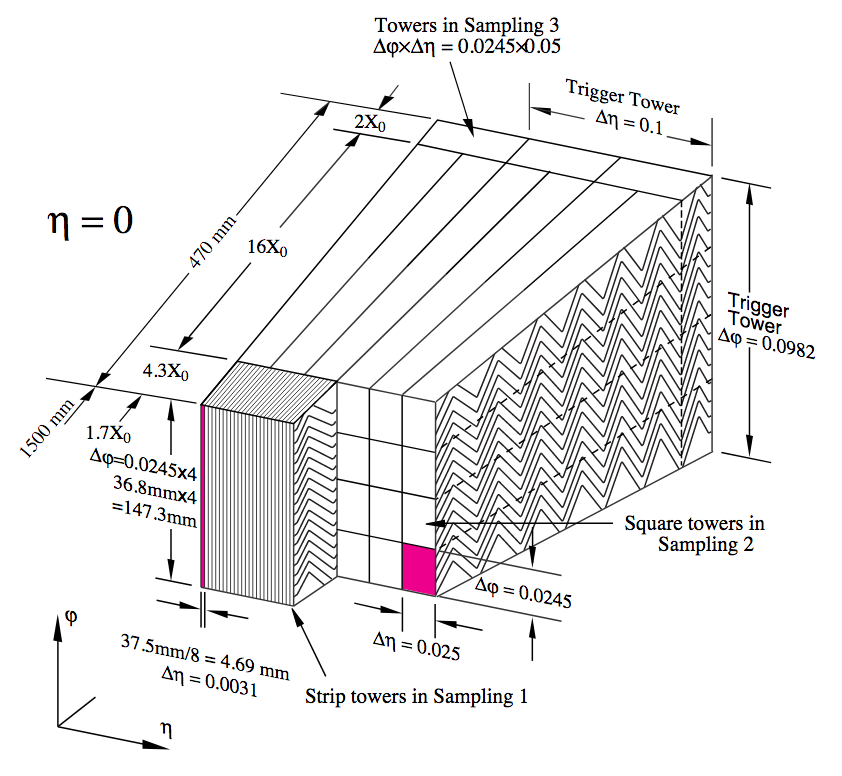
\includegraphics[width=0.6\textwidth]{figures/chapter2/calorimeters/atlas_em_calo_barrel}
        \raisebox{1.5cm}{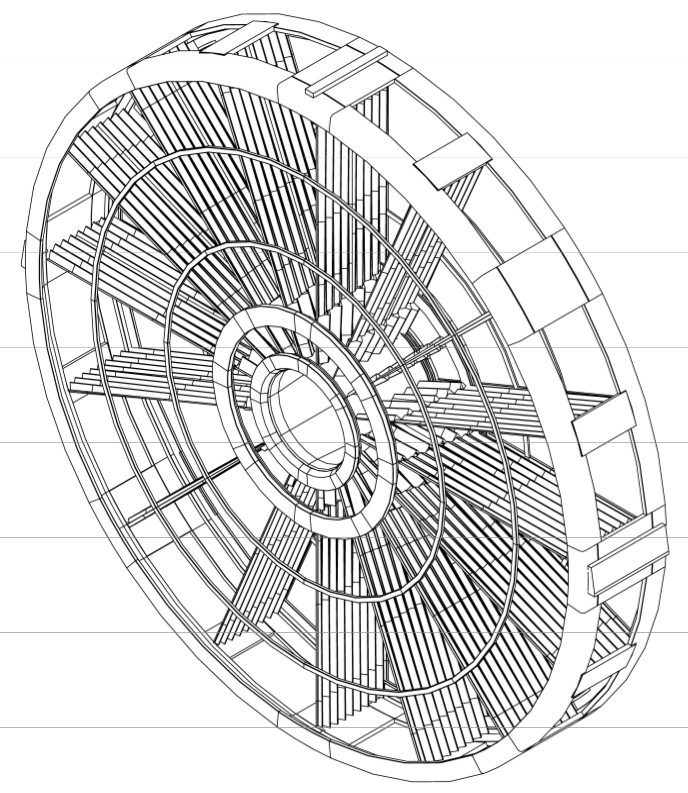
\includegraphics[width=0.3\textwidth]{figures/chapter2/calorimeters/atlas_em_calo_endcap}}
        \caption{
            \textbf{\textit{Left}}: Cut-away view of the barrel electromagnetic calorimeter and its accordian
                structure. Indicated are
                the geometry and absorption properties of the three sampling layers.
                Also indicated is the granularity of the electrode readout in $\Delta \phi \times \Delta \eta$
                in each layer.
            \textbf{\textit{Right}}: Diagram of the electromagnetic end-cap calorimeter accordian wheel structure
                (only a sub-set of the accordian structure is shown).
        }
        \label{fig:em_calo_section}
    \end{center}
\end{figure}

\FloatBarrier
\subsubsection{Hadronic Calorimeter}
\label{sec:calo_had}

The barrel section of the hadronic calorimeter is composed of a
lead/scintillating-tile type detector whereas the end-cap hadronic
calorimeter is based on copper/LAr-based technology.

The lead/scintillating-tile calorimeter (the `tile calorimeter') is located just beyond
the EM calorimeter.
It is composed of a barrel section, covering $\lvert \eta \rvert < 1.0$,
and two extended barrels that cover $0.8 < \lvert \eta \rvert < 1.7$ (see Figure~\ref{fig:atlas_calorimeters_cutaway}).
It is a sampling calorimeter using steel as the passive absorber and scintillating
plastic tiles as the active media.
The tile calorimeter is composed of modules in which the scintillating
tiles are situated in $(r-\phi)$ within the steel absorbers, as shown in Figure~\ref{fig:tile_calo}.
The detector is segmented radially into three layers and the readout of the
scintillation light, using wavelength-shifting fibers that are fed into photomultiplier tubes (PMT)
situated along the outer radii, is organized in a projective
geometry, also illustrated in Figure~\ref{fig:tile_calo}.
In the barrel (extended barrel) section, most of the hadronic energy is captured by the first (last) two
layers which account for $\approx 5.5$ ($6$) hadronic interaction lengths ($\lambda$)
of the $\approx 7$ in total.

The hadronic end-cap (HEC) calorimeter consists of two wheels per end-cap, situated
behind the electromagnetic end-cap calorimeter, and
provides calorimetric coverage in the range $1.5 < \lvert \eta \rvert <3.2$.
A view of the HEC can be seen in Figures~\ref{fig:atlas_calorimeters_cutaway} and \ref{fig:fcal}.
The HEC calorimeter is built from layers of copper plates interleaved with 8.5\,mm LAr gaps
which provide the active medium for this sampling calorimeter.
The readout structure is obtained by dividing the gaps into separate drift zones for
which there are dedicated readout electrodes.
This readout structure is arranged in a projective geometry.

\begin{figure}[!htb]
    \begin{center}
        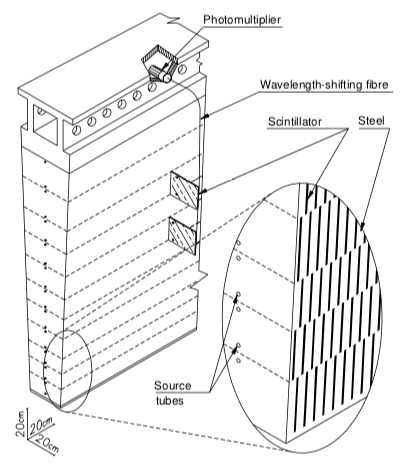
\includegraphics[width=0.4\textwidth]{figures/chapter2/calorimeters/atlas_tile_module}
        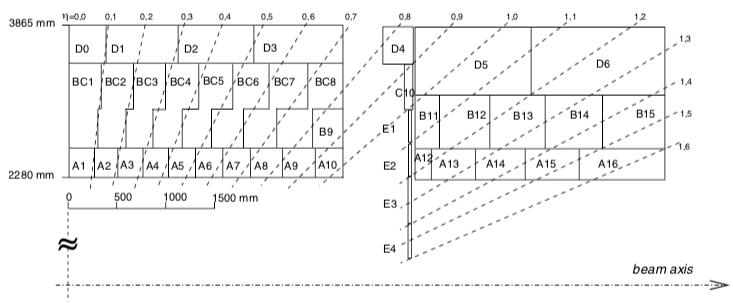
\includegraphics[width=0.9\textwidth]{figures/chapter2/calorimeters/atlas_tile_plan_view}
        \caption{
            \textbf{\textit{Top}}: A view of a tile calorimeter module with its interleaved steel
                absorbers and scintillating tiles and PMT readout. Also indicated are the source tubes
                through which radioactive Cesium (Cs) sources are passed for calibration purposes~\cite{Marjanovic:2018ohl}.
            \textbf{\textit{Bottom}}: Illustration of the segmentation of the projective readout of
                both the barrel and extended barrel tile calorimeter.
        }
        \label{fig:tile_calo}
    \end{center}
\end{figure}

\FloatBarrier
\subsubsection{Forward Calorimeter}
\label{sec:calo_forward}

The forward calorimeter (FCal) system~\cite{Artamonov_2008} provides calorimetric coverage to
high $\lvert \eta \rvert$, between $3.1 < \lvert \eta \rvert < 4.9$,
furthering the hermeticity of the detector.
As indicated in Figure~\ref{fig:fcal}, FCal consists of three layers in the
$z$ direction: an electromagnetic layer (FCal 1) and two hadronic layers (FCal 2 and FCal 3).
All three layers use LAr as the active medium but differ in their passive media.
FCal 1 uses copper for its absorber, chosen for its heat removal properties,
while FCal 2 and FCal 3 use tungsten, chosen to provide high containment and
minimisation of the lateral spread of hadronic showers.
The FCal modules consist of matrices of the passive material with regularly
spaced readout tubes  oriented parallel to the beam-pipe that are filled with the cooled LAr.

\begin{figure}[!htb]
    \begin{center}
        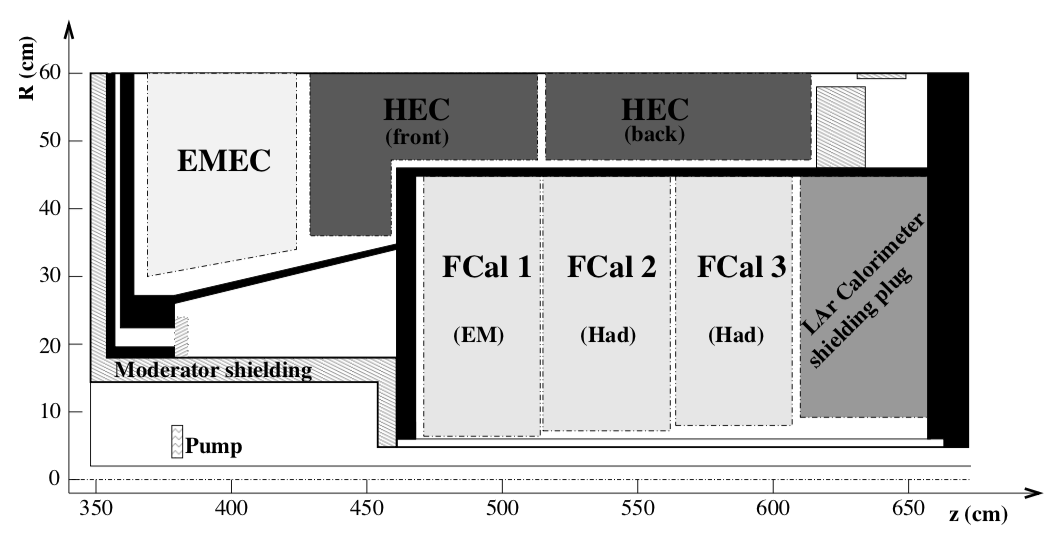
\includegraphics[width=0.65\textwidth]{figures/chapter2/calorimeters/atlas_fcal}
        \caption{
            View of the forward calorimeter (FCal) system. Portions of the electromagnetic
            and hadronic end-cap systems are also shown.
        }
        \label{fig:fcal}
    \end{center}
\end{figure}


%%%%%%%%%%%%%%%%%%%%%%%%%%%%%%%%%%%%%%%%%%%%%%%%%%%%%%%%%%%%%%%%%%%%%
%%%%%%%%%%%%%%%%%%%%%%%%%%%%%%%%%%%%%%%%%%%%%%%%%%%%%%%%%%%%%%%%%%%%%
%
% MUON SPECTROMETER
%
%%%%%%%%%%%%%%%%%%%%%%%%%%%%%%%%%%%%%%%%%%%%%%%%%%%%%%%%%%%%%%%%%%%%%
%%%%%%%%%%%%%%%%%%%%%%%%%%%%%%%%%%%%%%%%%%%%%%%%%%%%%%%%%%%%%%%%%%%%%
\subsection{The Muon Spectrometer}
\label{sec:ms}

Surrounding the calorimeters is the muon spectrometer (MS)~\cite{CERN-LHCC-97-022}, responsible
for the detection of high-momentum, minimum-ionizing muons originating from the $pp$ interaction.
The MS is based on the magnetic deflection of muon tracks, allowing for their
momentum determination.
The bending of the muon trajectories is provided by the large
superconducting air-core toroid magnet system, illustrated in Figure~\ref{fig:atlas_magnet_system},
consisting of a large barrel toroid over the range $\lvert \eta \rvert < 1.4$
and end-cap toroid systems in the range $1.6 < \lvert \eta \rvert < 2.7$.
The superconducting toroid magnet provides an average field of $4\,$T.
The magnetic field bending strength is roughly constant in $\eta$, except in the
region in which the transition between the barrel and end-cap toroids takes place
($1.4 < \lvert \eta \rvert < 1.6$).
A view of the ATLAS detector is shown in Figure~\ref{fig:atlas_in_cavern},
where it can be seen that the volume enclosed by the MS takes up most of the available volume
outside of the calorimeter systems in the underground experimental cavern at Point 1.
It should be noted that the overall design of the superconducting toroid structure,
dictated by the performance requirements of the MS, is what gives ATLAS its large size and essentially
drove the original design of all subdetectors discussed in the previous sections.

There are four types of gaseous radiation detector used in the MS, and their chamber
layout is based on the concept of projective towers.
The chambers follow the structure of the toroid magnet structure and have a 16-fold segmentation
in azimuth, shown in Figure~\ref{fig:muon_segmentation}.
They are arranged in large and small sectors, with the large sectors covering
the regions between the coils of the toroid and the small sectors the azimuthal range
in which the coils sit.
The detector types can be broken into two classes and are either
\textit{precision} or \textit{trigger} chambers.
The precision chambers allow for
the precise measurement the muon tracks as they traverse the MS, specifically the
precise measurement in the bending plane of these tracks so as to allow for accurate
determination of the muon momenta through their curvature.
The trigger chambers have fast signal formation and readout times, allowing for
accurate assignment of a passing muon to a specific $pp$ bunch crossing.
Both types of detectors exist in the barrel and end-cap \textit{stations} of the
MS and there are typically at least three layers of precision-type chambers over the
entire $\lvert \eta \rvert$ range of the MS in order to allow for the sagitta measurement
of the muon tracks necessary for momentum determination.
The layout of these detectors, in both the barrel and end-cap, is shown in
Figure~\ref{fig:muon_plan_view_eta}.

\begin{figure}[!htb]
    \begin{center}
        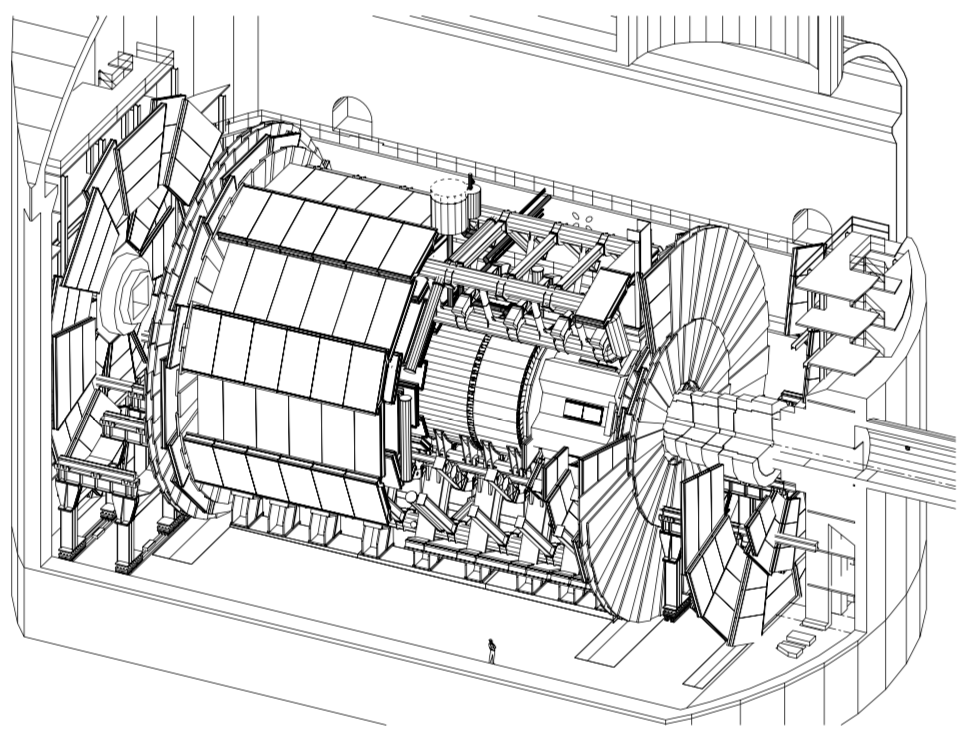
\includegraphics[width=0.8\textwidth]{figures/chapter2/atlas_in_cavern}
        \caption{
            A view of the ATLAS detector inside the underground experimental area
            UX15.
            The cut-away view exposes the toroid structure as well as the
            calorimeter system.
            Notice that the outermost muon stations in the forward regions are located
            at the extreme ends of the cavern.
            {\color{red}{Should move this figure either above or entirely}}
        }
        \label{fig:atlas_in_cavern}
    \end{center}
\end{figure}

\begin{figure}[!htb]
    \begin{center}
        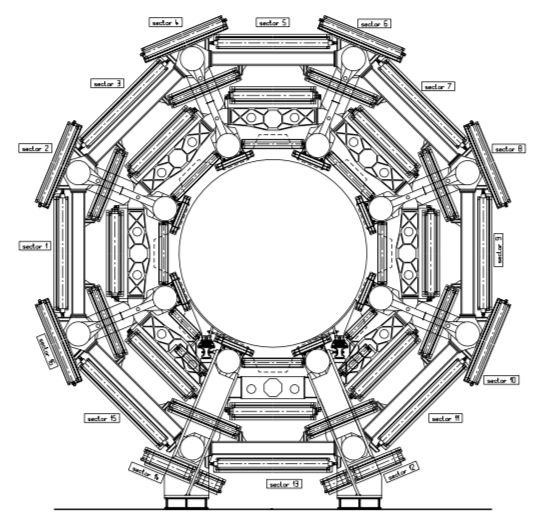
\includegraphics[width=0.4\textwidth]{figures/chapter2/muon_spec/atlas_muon_barrel}
        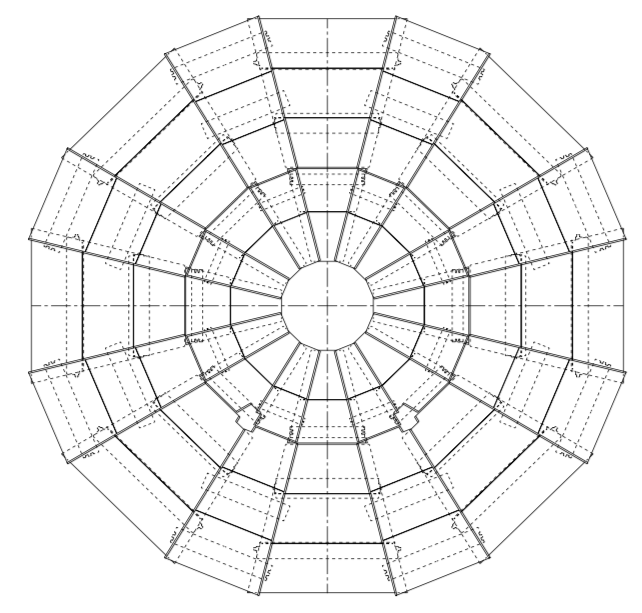
\includegraphics[width=0.35\textwidth]{figures/chapter2/muon_spec/atlas_muon_endcap}
        \caption{
            View of the 16-fold segmentation of the muon spectrometer in the barrel (\textit{left})
            and end-cap (\textit{right}).
            Clearly seen in both is the arrangment of the detector chambers into large and
            small sectors, allowing for complete coverage in azimuth.
            The view of the end-cap is that only of the MDT chambers located at $z\approx13$\,m.
        }
        \label{fig:muon_segmentation}
    \end{center}
\end{figure}

\begin{figure}[!htb]
    \begin{center}
        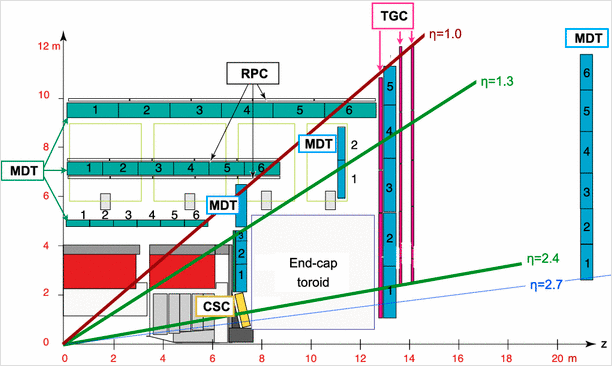
\includegraphics[width=0.8\textwidth]{figures/chapter2/muon_spec/atlas_muon_plan_view_eta}
        \caption{
            A view in the $r-z$ plane of a quadrant of the muon spectrometer (MS).
            Indicated by color are the four detector technologies used in the MS:
            MDT (blue), RPC (grey), TGC (red), and CSC (yellow).
            The light grey boxes at $6 < r < 9$\,m indicate the location of the
            barrel toroid structures.
            Also shown are the envelopes in $\lvert \eta \rvert$ of the barrel,
            small wheel, and big wheel sections of the MS.
        }
        \label{fig:muon_plan_view_eta}
    \end{center}
\end{figure}
\FloatBarrier


\begin{figure}[!htb]
    \begin{center}
        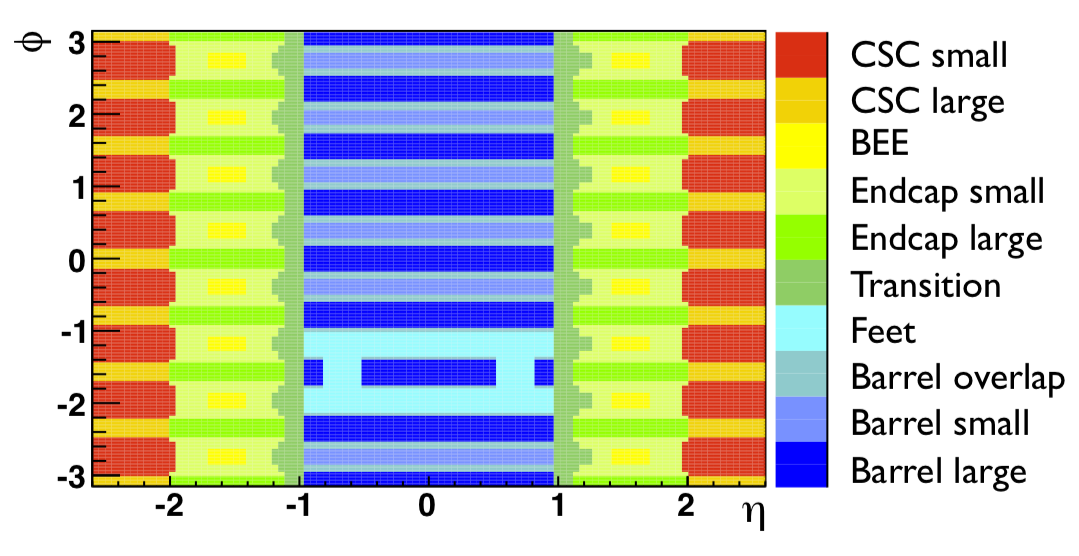
\includegraphics[width=0.7\textwidth]{figures/chapter2/muon_spec/atlas_muon_overlap}
        \caption{
        }
        \label{fig:muon_overlap}
    \end{center}
\end{figure}

\begin{figure}[!htb]
    \begin{center}
        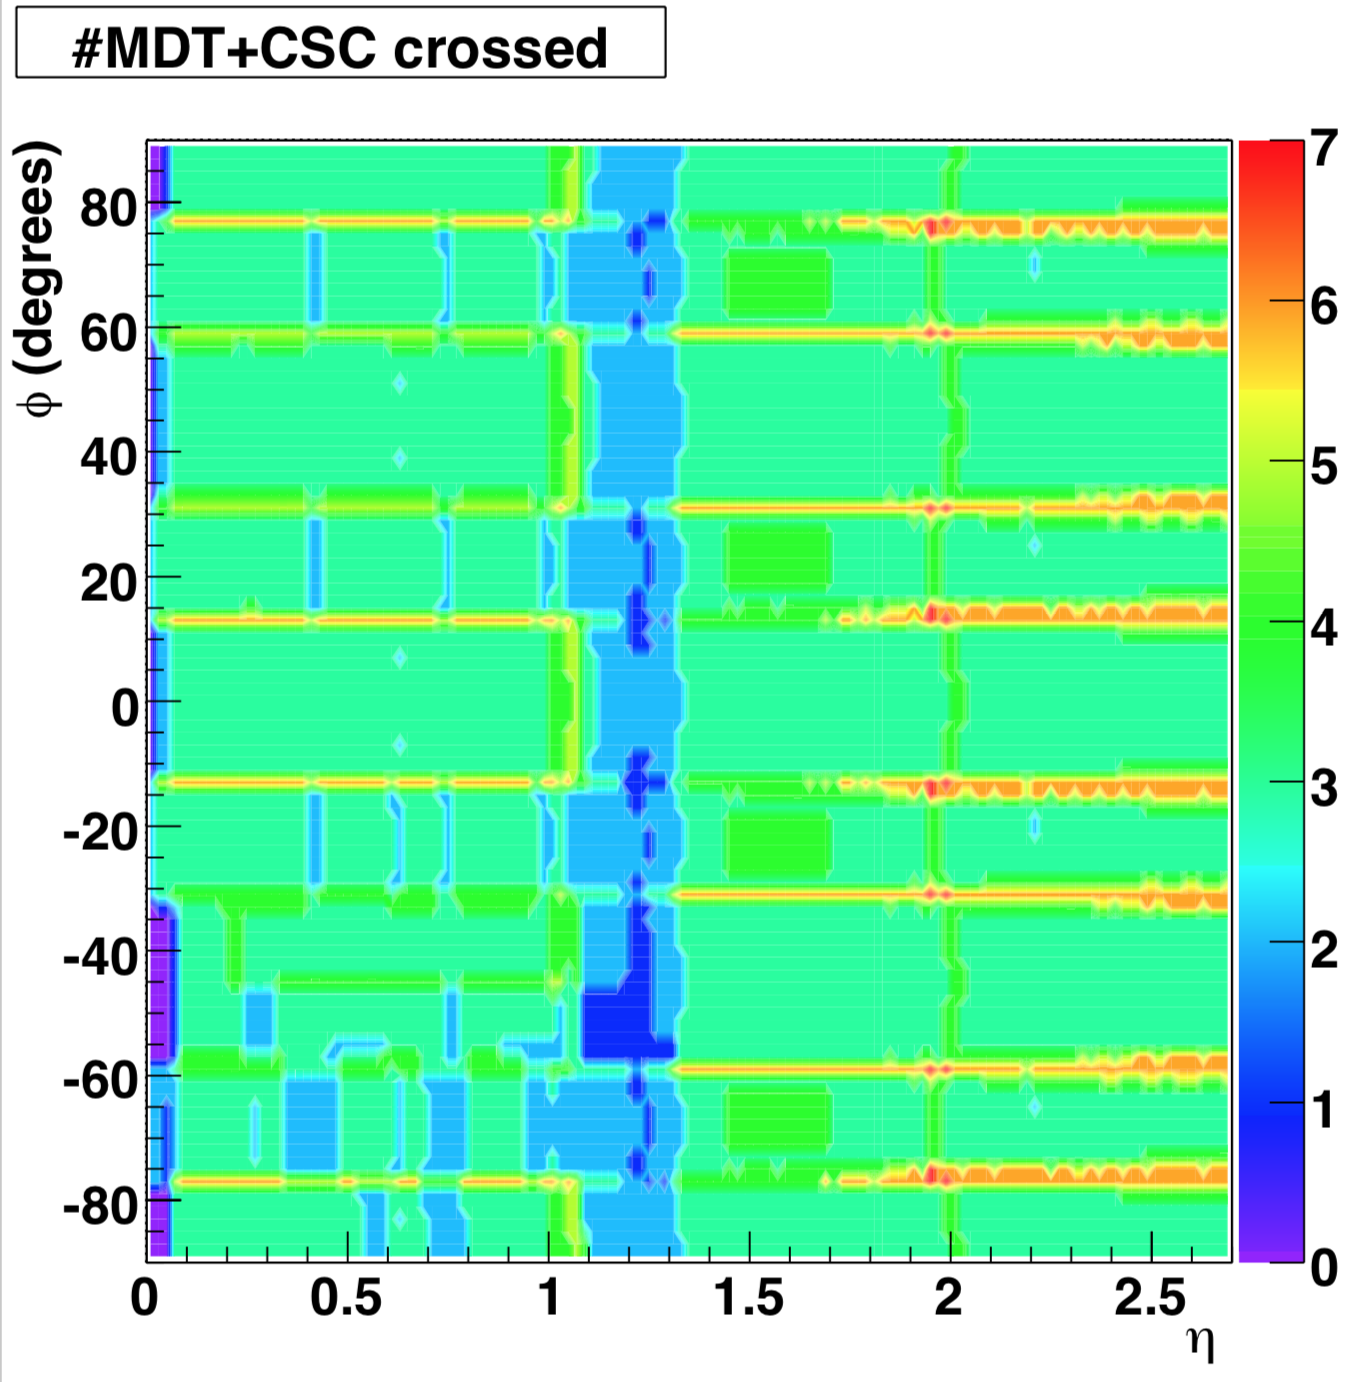
\includegraphics[width=0.7\textwidth]{figures/chapter2/muon_spec/atlas_ms_nchamber_crossed}
        \caption{
        }
        \label{fig:muon_nchambers_crossed}
    \end{center}
\end{figure}


\subsubsection{Precision Muon Chambers}
\label{sec:muon_precision}

\begin{figure}[!htb]
    \begin{center}
        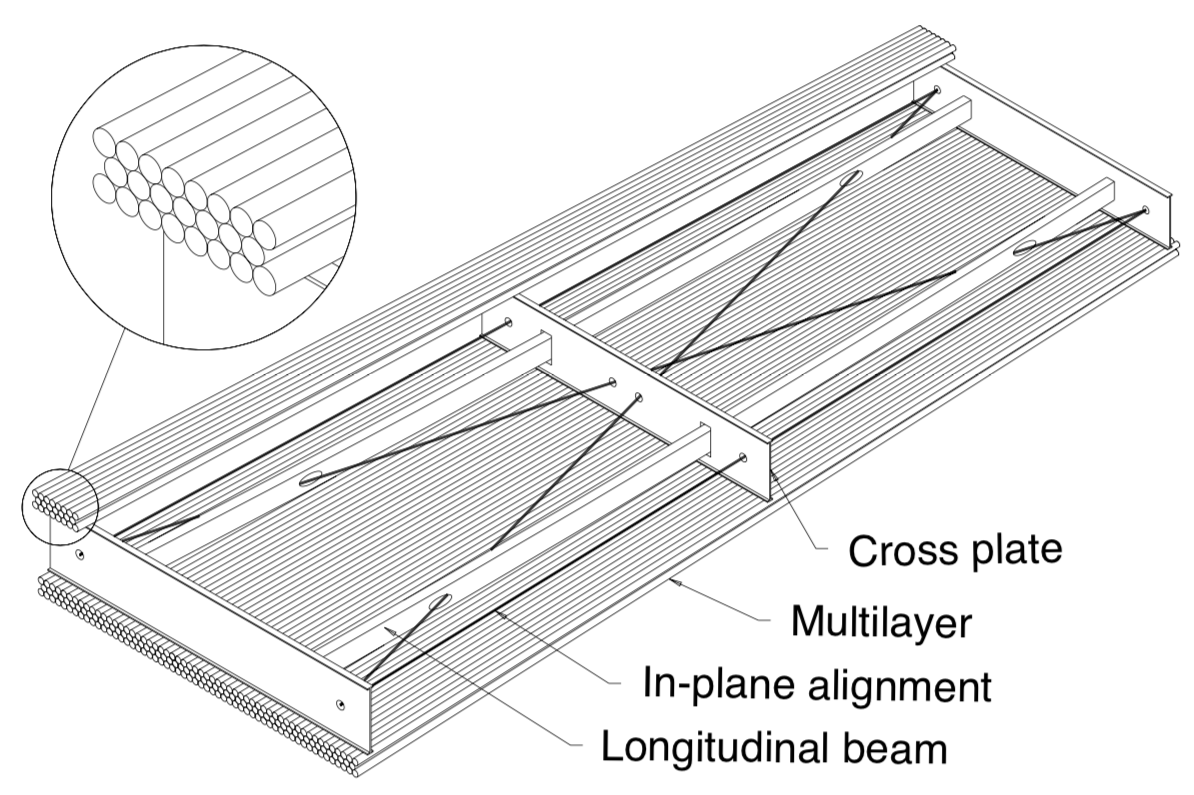
\includegraphics[width=0.5\textwidth]{figures/chapter2/muon_spec/mdt_chamber}
        \raisebox{1.22cm}{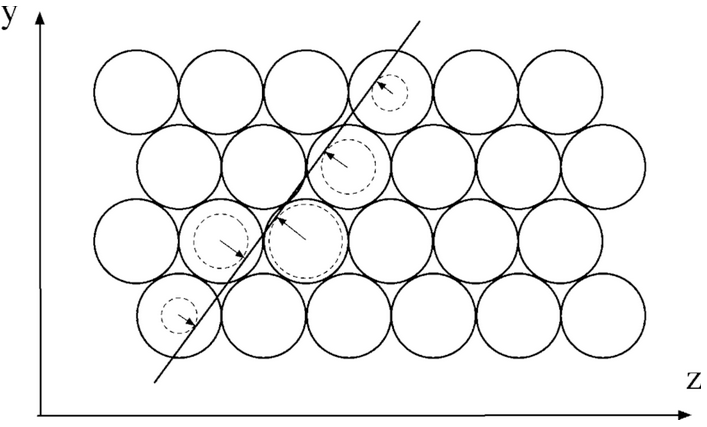
\includegraphics[width=0.32\textwidth]{figures/chapter2/muon_spec/mdt_trackfit}}
        \caption{
            \textit{Left}: Illustration of a double-multilayer MDT chamber with its internal alignment
                and support structure exposed. A zoom-in on the multilayer of MDT tubes is shown.
            \textit{Right}: Illustration of the multilayer MDT tracklet-fitting algorithm~\cite{MDTtrackfit}.
        }
        \label{fig:mdt_chamber}
    \end{center}
\end{figure}

\begin{figure}[!htb]
    \begin{center}
        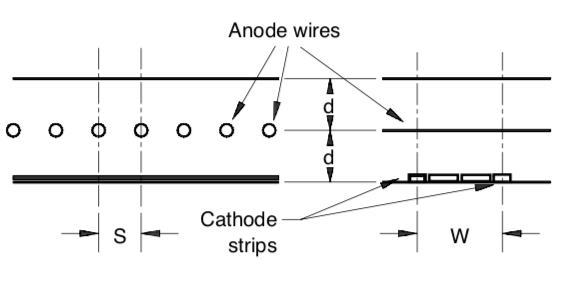
\includegraphics[width=0.55\textwidth]{figures/chapter2/muon_spec/csc_chamber}
        \caption{
            Diagram showing the main components of a cathode-strip chamber (CSC).
            On the \textit{left} (\textit{right}) is a view parallel (perpendicular) to the anode
            wires and perpendicular (parallel) to the cathode strips.
        }
        \label{fig:csc_chamber}
    \end{center}
\end{figure}

\subsubsection{Muon Trigger Chambers}
\label{sec:muon_trigger}

\begin{figure}[!htb]
    \begin{center}
        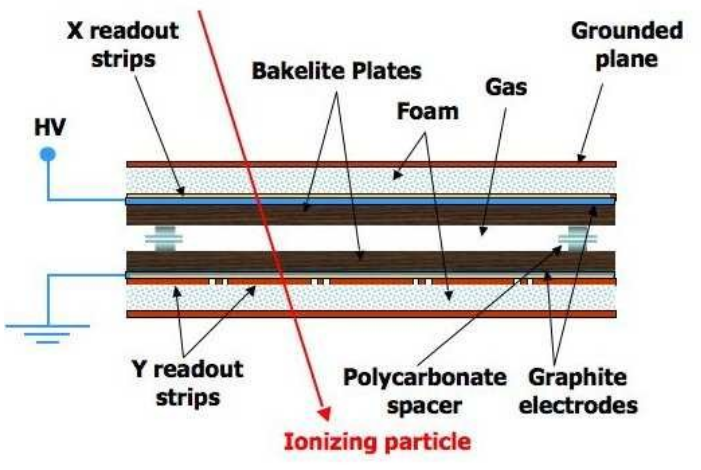
\includegraphics[width=0.5\textwidth]{figures/chapter2/muon_spec/rpc_chamber}
        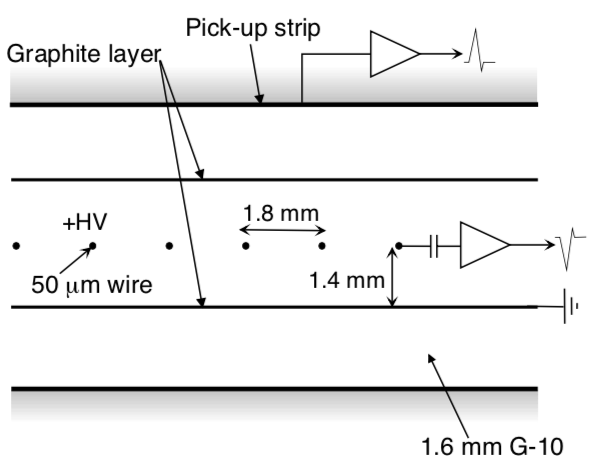
\includegraphics[width=0.38\textwidth]{figures/chapter2/muon_spec/tgc_chamber}
        \caption{
            \textit{Left}: Illustration of a resistive plate chamber (RPC) and its principle of operation.
            \textit{Right}: Diagram showing the main components of a thin-gap chamber (TGC).
        }
        \label{fig:muon_trigger_chamber}
    \end{center}
\end{figure}


%%%%%%%%%%%%%%%%%%%%%%%%%%%%%%%%%%%%%%%%%%%%%%%%%%%%%%%%%%%%%%%%%%%%%
%%%%%%%%%%%%%%%%%%%%%%%%%%%%%%%%%%%%%%%%%%%%%%%%%%%%%%%%%%%%%%%%%%%%%
%
% TDAQ
%
%%%%%%%%%%%%%%%%%%%%%%%%%%%%%%%%%%%%%%%%%%%%%%%%%%%%%%%%%%%%%%%%%%%%%
%%%%%%%%%%%%%%%%%%%%%%%%%%%%%%%%%%%%%%%%%%%%%%%%%%%%%%%%%%%%%%%%%%%%%
\subsection{Trigger and Data Acquisition}
\label{sec:tdaq}

During Run-II operation between 2015--2018, the LHC delivered $pp$ collisions to ATLAS at instantaneous luminosities of
$10^{34}$\,cm$^{-2}$s$^{-1}$, at a bunch spacing of 25\,ns, giving 33.7 $pp$ interactions per bunch crossing on average
(see Figure~\ref{fig:int_lumi_multiyear}).
These values correspond to roughly $10^9$ $pp$ interactions per second.
It is not possible for the ATLAS detector and data storage facilities to both respond to and record every one of these interactions.
In fact, from a physics perspective it is not necssarily desirable to record every single interaction.
The vast majority of such interactions arise from uninteresting, soft collision processes which are not likely
to contain, for example, decays of Higgs bosons or of new particles not accounted for in the SM.
For this reason, the ATLAS detector employs an \textit{online}\footnote{The `online' environment refers to that of the
ATLAS detector during runtime. The `offline' environment refers to anytime in which the data being inspected
or analysed is not \textit{at that time} being recorded by ATLAS but instead has already been stored to permanent storage
and is readily accessible at any time.}
selection strategy to select potentially interesting candidate events to be further processed and considered
for permanent storage. This online selection strategy is referred to as the \textit{trigger} system~\cite{Jenni:616089}.

The ATLAS Run-II trigger system consists of two levels: a hardware-based low-level
trigger, referred to as the \textit{Level-1} (L1) trigger, and a second level software-based high-level trigger (HLT)~\cite{PanduroVazquez:2244345}.
The L1 trigger uses relatively coarse-grained measurements from the calorimeters and MS.
It performs the first level of selection, reducing the initial input 40\,MHz rate of events by
accepting events at a maximal rate of 100\,kHz.
The L1 trigger performs searches for coarse proxies of interesting physics objects: leptons, photons, and jets.
It triggers on electrons and photons based on energy deposits in the EM calorimeter, limited to $\lvert \eta \rvert < 2.5$.
The hadronic calorimeter provides jet candidates to the L1 trigger system via calorimeter `towers' made up of
trigger elements constructed by a sliding window algorithm.
Each trigger element is constructed by calculating energy sums of calorimeter cells in $\eta - \phi$.
Muon-based L1 triggers are based on coincidences of hits along the layers of the MS that form
projective towers, or \textit{roads}, consistent with high-\pT~muons.

The candidate events selected by the L1 trigger system are forwarded to the HLT.
The HLT system is composed of a Level 2 (L2) trigger and the event filter (EF).
The L2 system is similar to the L1 trigger, but performs more refined measurements on the objects and
regions of the detector that resulted in the initial L1 trigger's decision to accept the event.
The EF is purely software based, using the ATLAS Athena reconstruction framework~\cite{AthenaRef}
to perform high level object reconstruction and identification using algorithms similar to those used
in the offline environment ({\color{red}{Section XXX}}).
The HLT accept rate is roughly 1\,kHz.
The accepted events are sent to CERN's permanent storage facilities and are made ready for the offline analysis.
An overview of the trigger system is shown in Figure~\ref{fig:run2_trigger}.


\begin{figure}[!htb]
    \begin{center}
        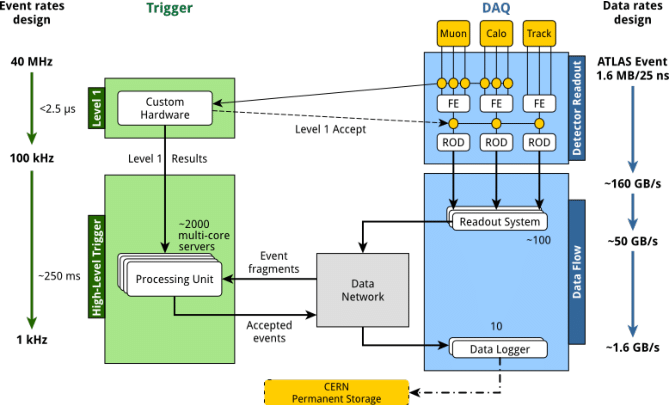
\includegraphics[width=0.7\textwidth]{figures/chapter2/tdaq/atlas_run2_trigger_system}
        \caption{
            Overview of the ATLAS Run-II trigger and data-acquisition architecture.
            Data from the muon and calorimeter systems are used for the Level 1 (L1) trigger, reducing
            the input event rate from 40\,MHz to 100\,kHz.
            The data accepted by the L1 trigger are forwarded to the readout drivers (RODs)~\cite{Jenni:616089}
            which, among other things, re-shuffle the raw data into the standardized ATLAS event format~\cite{Bee:683741}.
            The events selected by the HLT at a rate of 1\,kHz are pulled from the RODs and then forwarded to the permanent
            storage.
            Figure taken from Ref.~\cite{PanduroVazquez:2244345}.
        }
        \label{fig:run2_trigger}
    \end{center}
\end{figure}



% ... and so on

% if doing minimal compilation, set the page counter to start at the document meat -- otherwise use the "\preliminarypages" command above
\setcounter{page}{0}
%\chapter{The Standard Model of Particle Physics}

%\epigraph{\textit{So it goes...}}{---Kurt Vonnegut, \textit{Slaughterhouse
%		Five}}
	
%\epigraph{\textit{Science is a miracle.}}{--Ron Swanson}

\epigraph{\textit{If you wish to make an apple pie from scratch, you must first invent the universe.}}{--Carl Sagan, \textit{Cosmos: A Personal Voyage}}


As it stands, what has become known as the `Standard Model (SM) of Particle Physics'
is nothing less than one of the greatest achievments of mankind, due to both
the magnitude by which it has changed our perception of the underlying
nature of the universe and to the clever methods and tinkerings by which this
nature was unveiled by many clever physicists whose history has become veritable lore.
In terms of imagination and insight, it is second only to the special and general theories of relativity --
though the fields are nevertheless intricately intertwined.
%{\color{red}{The latter, though, being put forth by essentially a single person and the latter by a great many...}}.

Not considering the scientific progress made in the $18^{th}$ and $19^{th}$ centuries, and
ignoring the ancient Greeks despite their fabled invention of atomic theory,
the physical insights and major work that led to the current picture of elementary particle
physics described by the SM began with the \textit{annus mirabilis} papers of Albert
Einstein in the year 1905~\cite{einsteinPEE,einsteinSpecial,einsteinEnergyMass}.
In these papers, Einstein was able to shed light on the quantization of electromagnetic
radiation (building off of the seminal work of Max Planck~\cite{planckBlackBody})
and introduce the special theory of relativity.
These works laid the conceptual
and philosophical groundwork for the major breakthroughs in fundamental physics
of $20^{th}$ century physics: from the `old quantum theory' of Bohr and Sommerfeld
in the early 1900's to the equivalent wavefunction and matrix-mechanics formulations
of Schr{\"o}dinger and Heisenberg that
coalesced into `modern' quantum mechanics in the mid-1920's.
The modern approach, non-relativistic at its heart, provided a sufficient mathematical
and interpretable framework in which to work and match predictions to observed phenomena, old
and new. It has for the most part remained unchanged and is the quantum mechanics that is taught to
students at both the undergraduate and graduate level to this very day.
It is the theory that has since revolutionised all aspects of the physical sciences and
technologies that dictate our everyday-lives.
In the mid-1920's, however, despite
large efforts put forth by the forbears of modern quantum mechanics, the quantum-mechanical
world had yet to be made consistent with Einstein's theory of relativity --- a requirement
that must be met for all consistent physical theories of nature.
It was the insight of Paul Dirac who was finally able to successfully
marry the theory of the quantum with that of relativity when he introduced
his relativistic quantum-mechanical treatment of the electron in 1927 and 1928~\cite{diracEquation,Dirac:1927dy}.\footnote{
A complete history of the people and ideas involved in the development of the modern
theory of Quantum Mechanics can be found in references ~\cite{boffiRiseOfQM,historyQM},
and the references therein.
}
This work provided the starting point for a decades-long search of a consistent quantum-mechanical
and relativistic treatment of electrodynamics, known as \textit{quantum electrodynamics} (QED).
The search for QED ended at the end of the 1940's with the groundbreaking work of Dyson, Feynman, Schwinger, and Tomanaga~\cite{qedTomonaga,qedFeynman0,qedFeynman1,qedFeynman2,qedSchwinger0,qedSchwinger1,qedDyson0,qedDyson1} that introduced the covariant and gauge invariant
formulation of QED --- the first such relativistic quantum field theory (QFT).
QED allowed the physcists to make predictions that agreed with observation at unprecedented levels
of accuracy and has since led to the adoption of its language and mathematical toolkit as the
foundational framework in which to construct models that accurately describe nature.\footnote{
	For a complete discussion of the developments leading up to QED, see the fabulous
	book by S. Schweber~\cite{Schweber:1994qa}.	
}
The SM is no less than an ultimate conclusion of these works: a consistent set of relativistic
quantum field theories, using the language developed by Feynman et al.,
that describes essentially all aspects of the known particles and forces that make up the 
observed universe.


\section{Particles and Forces}

Here we introduce the SM particle content and provide a description of the interactions that
link the particles together.


\begin{table}[!htb]
    \caption{
        The particle content of the SM and their transformation
        properties under the SM gauge groups, prior to electroweak symmetry breaking.
        The representations of each of the gauge groups are shown in the three-right
        columns. The \Uone symmetry of weak-hypercharge transformations is one-dimensional
        and the column gives the weak-hypercharge $\mathcal{Y}$ associated with each
        field. For \SUthree and \SUtwo, $\mathbf{1}$ refers to the field belonging to
        the associated singlet representation, $\mathbf{2}$ to the doublet representation,
        $\mathbf{3}$ to the triplet representation, and $\mathbf{8}$ to the octet representation.
    }
    \begin{center}
        \begin{tabularx}{0.96\textwidth}{m{1em} c c c c c c }
        \toprule
        \hline
        & Field Label & Content & Spin & \Uone~($\mathcal{=Y}$) & \SUtwo & \SUthree \\
        \hline
        \rotatebox{90}{\hspace{-0.1cm}\textbf{Quarks} } 
         &   \makecell{\fieldQi \\ \fieldUri \\ \fieldDri} % FIELD
         &   \makecell{ (\fieldUl, \fieldDl), (\fieldCl, \fieldSl), (\fieldTl, \fieldBl) \\ \fieldUr \\ \fieldDr}% CONTENT
         &   \makecell{ $1/2$ \\ $1/2$ \\ $1/2$} % SPIN
         &   \makecell{ $1/6$ \\ $2/3$ \\ $-1/3$}% U(1)
         &   \makecell{ $\mathbf{2}$ \\ $\mathbf{1}$ \\ $\mathbf{1}$}% SU(2)
         &   \makecell{ $\mathbf{3}$ \\ $\mathbf{3}$ \\ $\mathbf{3}$}\\ % SU(3)
        %\cdashline{1-7}
        \rotatebox{90}{\hspace{-0.1cm}\textbf{Leptons} }
         &   \makecell{\fieldLi \\ \fieldEri} % FIELD
         &   \makecell{ (\fieldEl, \fieldNuEl), (\fieldMul, \fieldNuMul), (\fieldTaul, \fieldNuTaul) \\ \fieldEr, \fieldMur, \fieldTaur}% CONTENT
         &   \makecell{ $1/2$ \\ $1/2$ }% SPIN
         &   \makecell{ $1/2$ \\ $-1$ }% U(1)
         &   \makecell{ $\mathbf{2}$ \\ $\mathbf{1}$ }% SU(2)
         &   \makecell{ $\mathbf{1}$ \\ $\mathbf{1}$ } \\ % SU(3)
        \midrule
        \rotatebox{90}{\textbf{\stackanchor{Gauge}{Fields}} }
         &   \makecell{\fieldB \\ \fieldW \\ \fieldG } % FIELD
         &   \makecell{ \fieldB \\ (\fieldWone, \fieldWtwo, \fieldWthree) \\ \fieldG$_a$, $a\in[1,..,8]$ }% CONTENT
         &   \makecell{ $1$ \\ $1$ \\ $1$} % SPIN
         &   \makecell{ $0$ \\ $0$ \\ $0$}% U(1)
         &   \makecell{ $\mathbf{1}$ \\ $\mathbf{3}$ \\ $\mathbf{1}$}% SU(2)
         &   \makecell{ $\mathbf{1}$ \\ $\mathbf{1}$ \\ $\mathbf{8}$}\\ % SU(3)
        \midrule
        \rotatebox{90}{\textbf{\stackanchor{Higgs}{Field}}} 
         &   \makecell{\fieldPhi } % FIELD
         &   \makecell{ (\fieldPhip, \fieldPhizero) }% CONTENT
         &   \makecell{ $0$  } % SPIN
         &   \makecell{ $1/2$  }% U(1)
         &   \makecell{ $\mathbf{2}$ }% SU(2)
         &   \makecell{ $\mathbf{1}$ }\\ % SU(3)
        \hline
        \bottomrule
        \end{tabularx}
    \end{center}
    \label{tab:sm_content}
\end{table}


\begin{table}[!htb]
    \caption{
        The particle content of the SM after the process of
        electroweak symmetry breaking.
    }
    \begin{center}
        \begin{tabularx}{1\textwidth}{m{1em} c c c c }
        \toprule
        \hline
        & Physical Field & Q & Coupling & Mass [GeV] \\
        \hline
        \rotatebox{90}{\hspace{-0.1cm}\textbf{Quarks} } 
            & \makecell{ \quarkU, \quarkC, \quarkT \\ \quarkD, \quarkS, \quarkB} % FIELD
            & \makecell{ $2/3$ \\ $-1/3$ }% Q
            %& \makecell{ $\mathbf{3}$ \\ $\mathbf{3}$ } % SU(3)
            & \makecell{ ($y_i=$) $1\times10^{-5}$, $7\times10^{-3}$, $1$ \\ ($y_i=$) $3\times10^{-5}$, $5\times10^{-4}$, $0.02$ } % Coupling
            & \makecell{ $2\times10^{-3}$, $1.27$, $173$ \\ $4\times10^{-4}$, $0.10$, $4.18$ }\\% Mass
        \rotatebox{90}{\hspace{-0.1cm}\textbf{Leptons} } 
            & \makecell{ \leptonE, \leptonMu, \leptonTau \\ \neutrinoE, \neutrinoMu, \neutrinoTau } % FIELD
            & \makecell{ $-1$ \\ $0$ }% Q
            %& \makecell{ $\mathbf{1}$ \\ $\mathbf{1}$ } % SU(3)
            & \makecell{ ($y_i=$) $3\times10^{-7}$, $6\times10^{-4}$, $0.01$ \\ -- } % Coupling
            & \makecell{ $5\times10^{-4}$, $0.106$, $1.777$ \\ --}\\% Mass
        \midrule
        \rotatebox{90}{\textbf{Bosons} } 
            & \makecell{ \fieldPhoton \\ \fieldZ \\ (\fieldWp, \fieldWm) \\ \fieldG } % FIELD
            & \makecell{ $0$ \\ $0$ \\ $(+1,-1)$ \\ $0$ }% Q
            %& \makecell{ $\mathbf{1}$ \\ $\mathbf{1}$ \\ $\mathbf{1}$ \\ $\mathbf{8}$ } % SU(3)
            & \makecell{ $\alpha_{\text{EM}} \simeq 1/137$ \\ $\sin \theta_{W} \simeq 0.5$ \\ -- \\ $\alpha_s \simeq 0.1$ } % Coupling
            & \makecell{ $0$ \\ $91.2$ \\ $80.4$ \\  $0$}\\% Mass
        \midrule
        \rotatebox{90}{\textbf{Higgs} } 
            & \makecell{ \fieldH } % FIELD
            & \makecell{ $0$ }% Q
            %& \makecell{ $\mathbf{1}$ } % SU(3)
            & \makecell{ $\lambda$, $\mu$ } % Coupling
            & \makecell{ $125.09$ }\\% Mass

         %&   \makecell{ (\quarkUl, \quarkDl), (\quarkCl, \quarkSl), (\quarkTl, \quarkBl) \\ \quarkUr \\ \quarkDr}% CONTENT
         %&   \makecell{ $1/2$ \\ $1/2$ \\ $1/2$} % SPIN
         %&   \makecell{ $\mathbf{2}$ \\ $\mathbf{1}$ \\ $\mathbf{1}$}% SU(2)
         %&   \makecell{ $\mathbf{3}$ \\ $\mathbf{3}$ \\ $\mathbf{3}$}\\ % SU(3)
        %%\cdashline{1-7}
        %rotatebox{90}{\hspace{-0.1cm}\textbf{Leptons} }
         %&   \makecell{\quarkLi \\ \quarkEri} % FIELD
         %&   \makecell{ (\quarkEl, \quarkNuEl), (\quarkMul, \quarkNuMul), (\quarkTaul, \quarkNuTaul) \\ \quarkEr, \quarkMur, \quarkTaur}% CONTENT
         %&   \makecell{ $1/2$ \\ $1/2$ }% SPIN
         %&   \makecell{ $\mathbf{2}$ \\ $\mathbf{1}$ }% SU(2)
         %&   \makecell{ $\mathbf{1}$ \\ $\mathbf{1}$ } \\ % SU(3)
        %midrule
        %rotatebox{90}{\textbf{\stackanchor{Gauge}{Fields}} }
         %&   \makecell{\quarkB \\ \quarkW \\ \quarkG } % FIELD
         %&   \makecell{ \quarkB \\ (\quarkWone, \quarkWtwo, \quarkWthree) \\ \quarkG }% CONTENT
         %&   \makecell{ $1$ \\ $1$ \\ $1$} % SPIN
         %&   \makecell{ $\mathbf{1}$ \\ $\mathbf{3}$ \\ $\mathbf{1}$}% SU(2)
         %&   \makecell{ $\mathbf{1}$ \\ $\mathbf{1}$ \\ $\mathbf{8}$}\\ % SU(3)
        %midrule
        %rotatebox{90}{\textbf{\stackanchor{Higgs}{Field}}} 
         %&   \makecell{\quarkPhi } % FIELD
         %&   \makecell{ (\quarkPhip, \quarkPhizero) }% CONTENT
         %&   \makecell{ $0$  } % SPIN
         %&   \makecell{ $\mathbf{2}$ }% SU(2)
         %&   \makecell{ $\mathbf{1}$ }\\ % SU(3)
        \hline
        \bottomrule
        \end{tabularx}
    \end{center}
    \label{tab:sm_content}
\end{table}



\subsection{Gauge Theories}

\subsubsection{The Electroweak Theory}



\chapter{Experimental Setup}

%\epigraph{\textit{Nice piece of wood in that counter. Nicely planed. Like the way it curves there.}}{--Leopold Bloom, in James Joyce's \textit{Ulysses}}
\epigraph{\textit{I know of no more encouraging fact than the unquestionable ability
of man to elevate his life by a conscious endeavour. It is something to be able to paint a particular picture,
or to carve a statue, and so to make a few objects beautiful; but it is far more glorious to carve
and paint the very atmosphere and medium through which we look, which morally we can do.}}{--Henry David Throeau, \textit{Walden}}

The work to be described in the present thesis was done at CERN\footnote{
The acronym CERN was historically derived from `\textit{Conseil europ{\'e}en pour la recherche
nucl{\'e}aire'}. Nowadays, `CERN' has become a standalone name for the lab itself and
is currently referred to as the `\textit{Organisation europ{\'e}enne pour la recherche nucl{\'e}aire}'; or, in English: the
`\textit{European Organisation for Nuclear Research.}'}, the particle
physics laboratory located along the French-Swiss border just outside of Geneva, Switzerland.
CERN is comprised of almost 18,000 personnel, of which over 13,000 are researchers in the
field of experimental particle physics.
It is a truly international workplace, with the personnel comprised of representatives of over 110 nationalities
and who are either working directly
for CERN\footnote{Of the roughly 18,000 researchers in experimental particle physics, only about
5\% are employed directly by CERN itself.} or for their respective home institutions
--- universities or national labs ---
located across more than 70 countries worldwide~\cite{CERN-HR-STAFF-STAT-2018}.
These researchers will generally work at any of the independent experiments located along the various
beamlines that network throughout the CERN campus (see Fig.~\ref{fig:cern_complex}).

At the time of writing, there are four large experiments\footnote{For the most part, one can interchange the
words `detector' and `experiment' when referencing large-scale, long-term particle physics experiments such as those
that have taken place over the past few decades: the detectors tend to take on the role of representing
the entire collaboration of physicists, engineers and associated personnel, as well as the entire scope of the associated
research programs.} taking place currently at CERN, all located along the Large
Hadron Collider (LHC): ALICE~\cite{ALICECollab}, LHCb~\cite{LHCbCollab}, CMS~\cite{CMSCollab},
and ATLAS~\cite{ATLASCollab}. The CMS and ATLAS detectors are general purpose detectors, with broad
research programs, whereas the ALICE and LHCb detectors are specialised for the study of heavy-ion
collisions and $b$-hadron physics, respectively.

This chapter will present a brief introduction to the workings of the LHC in Section~\ref{sec:lhc}.
In Section~\ref{sec:atlas}, given that the present author is a member of the ATLAS collaboration,
a detailed description of the various components that make up the ATLAS detector will be presented.

%As the present author is a member of one of the two general-purpose experiments at CERN located
%along the Large Hadron Collider (LHC) -- the ATLAS experiment -- this chapter will present a
%brief introduction to the workings of the LHC (Section~\ref{sec:lhc}) and then describe in some
%detail the various components that make up the ATLAS detector (Section~\ref{sec:atlas}), the largest
%and most complex scientific piece of equipment ever 
%constructed by humans.\footnote{The ATLAS detector, along with its operation, is by far more complex
%than any previous human endeavour --- generally more complex than anything operated and enacted by NASA, for
%example. The only difference being the tolerance for failure: in the case of NASA space-based experiments and missions
%this tolerance approaches zero, whereas the terrestrial particle physics experiments happening at the
%LHC are generally accessible and amenable to errors.}


\begin{figure}[!htb]
    \begin{center}
        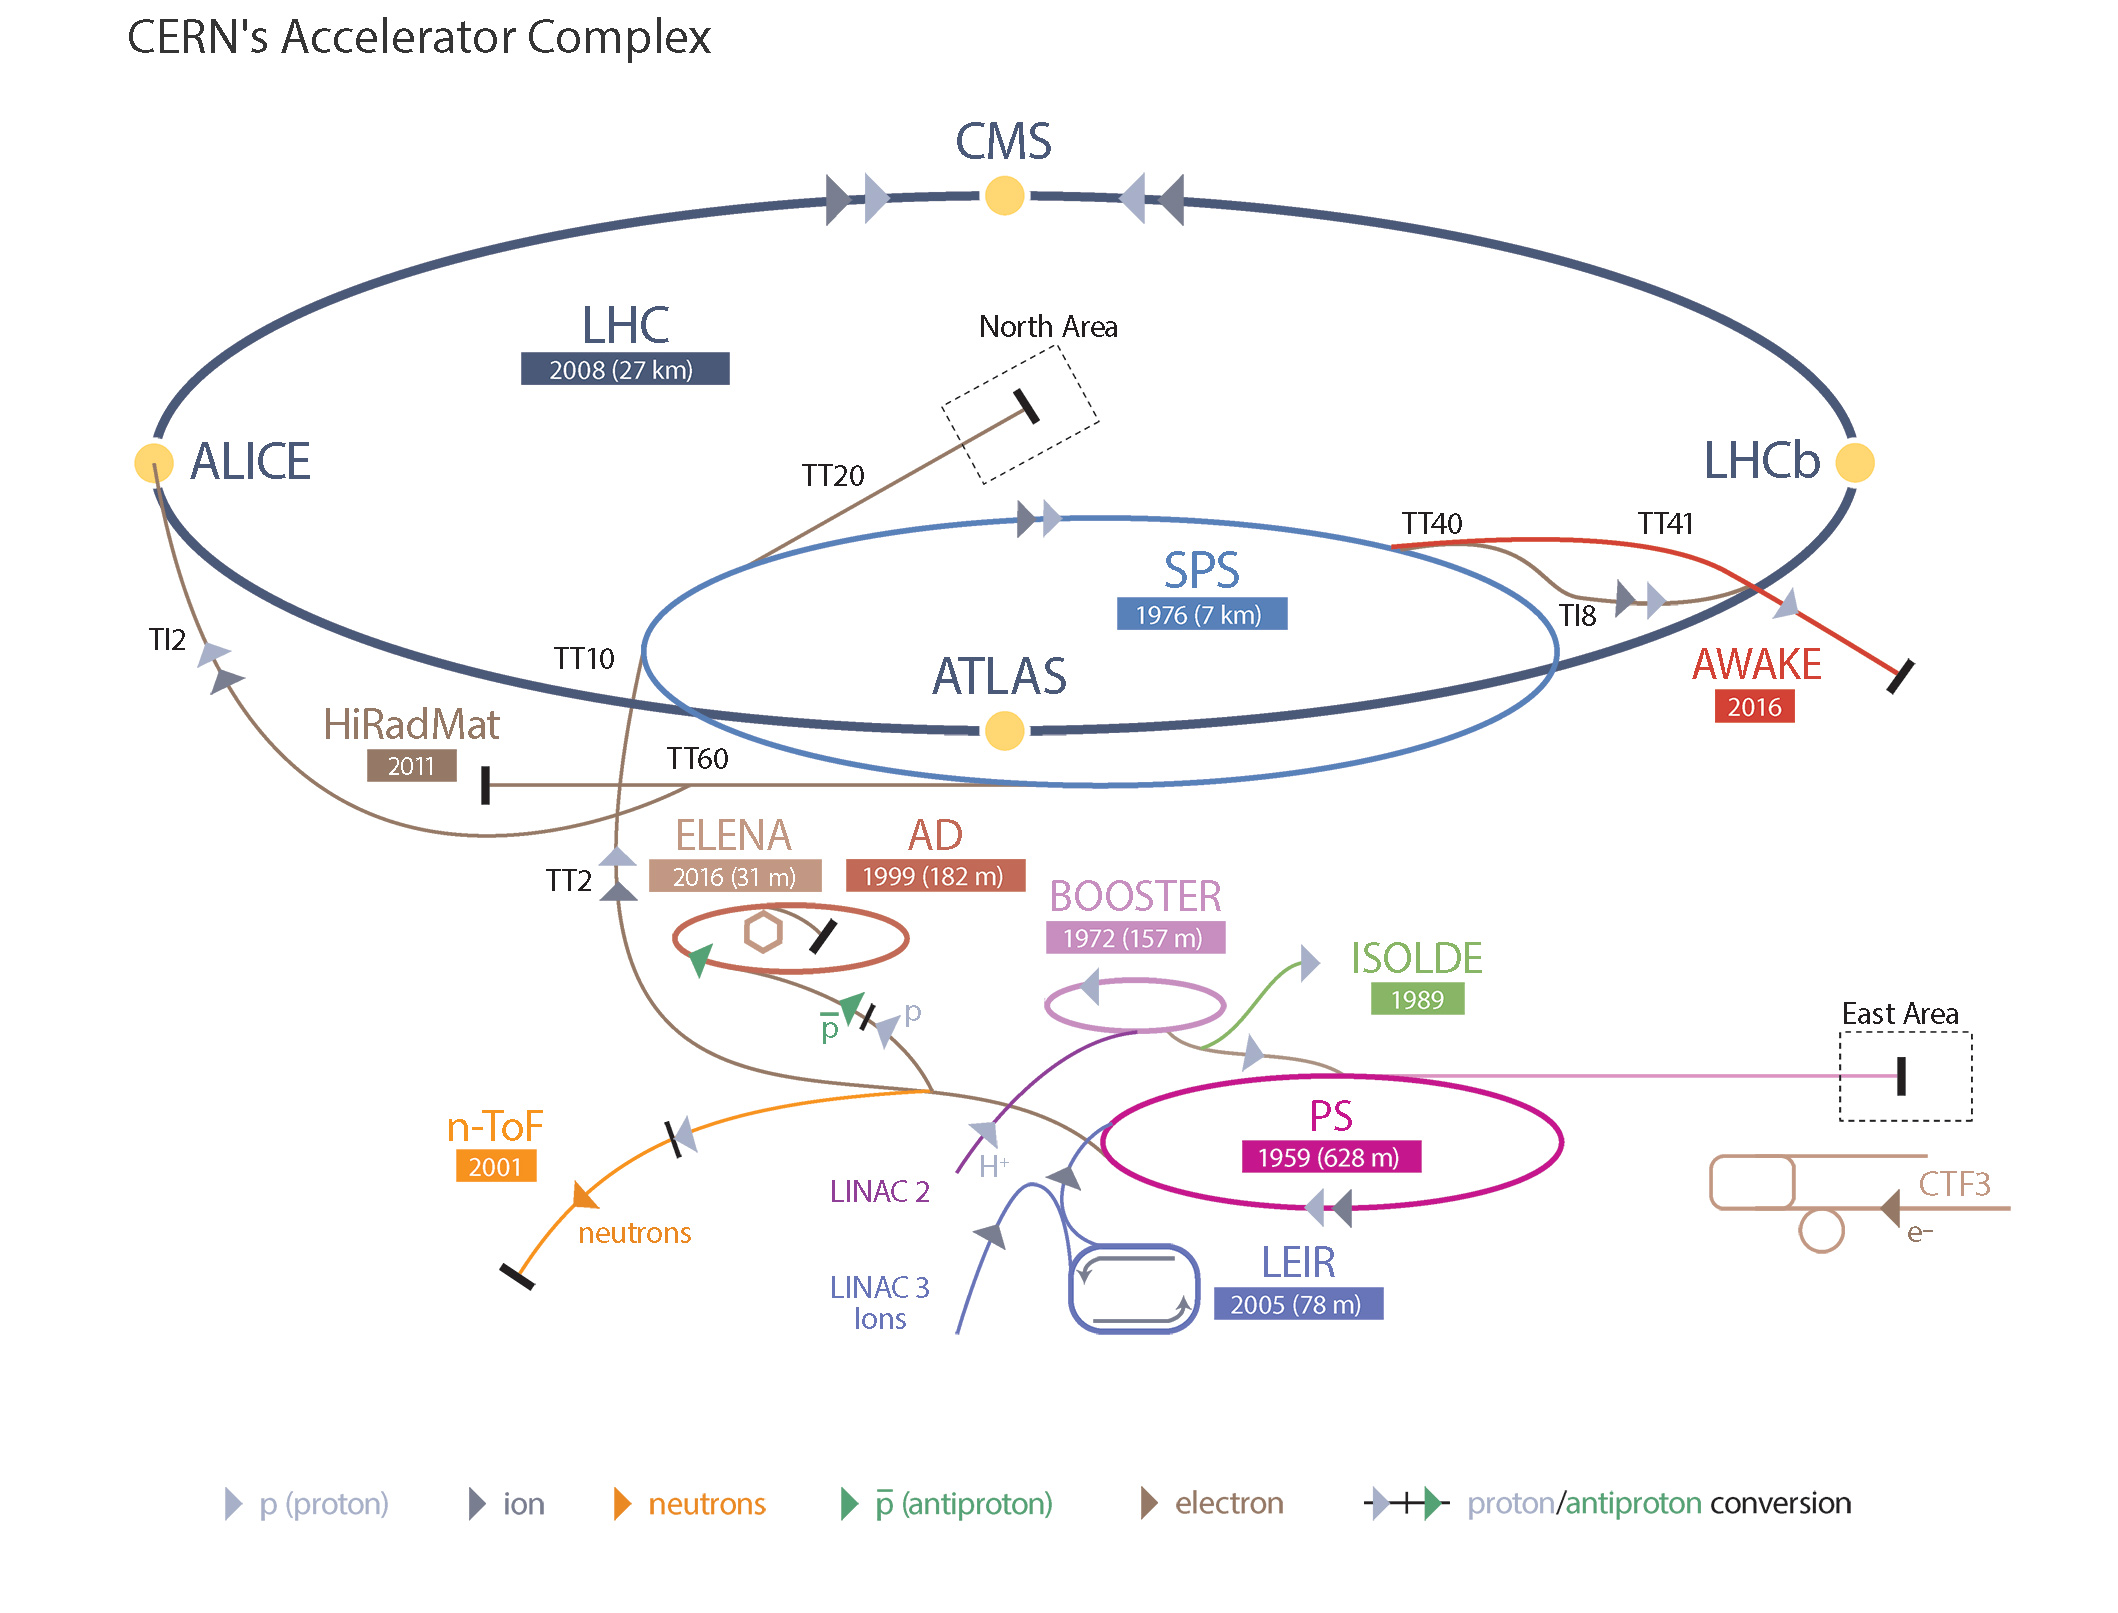
\includegraphics[width=0.8\textwidth]{figures/chapter2/cern_accelerator_complex2}
        \caption{
            Illustration of the various beamlines, accelerator and storage rings, and experimental
            points that the CERN accelerator complex is home to.
            The protons that circulate through the LHC, and that are eventually made to collide inside
            the ATLAS detector, follow the path: Linac 2 $\rightarrow$ Booster $\rightarrow$ Proton Synchotron (PS)
            $\rightarrow$ Super Proton Synchotron (SPS) $\rightarrow$ LHC.
        }
        \label{fig:cern_complex}
    \end{center}
\end{figure}


%%%%%%%%%%%%%%%%%%%%%%%%%%%%%%%%%%%%%%%%%%%%%%%%%%%%%%%%%%%%%%%%%%%
%%%%%%%%%%%%%%%%%%%%%%%%%%%%%%%%%%%%%%%%%%%%%%%%%%%%%%%%%%%%%%%%%%%
% sub-section describing the LHC
%%%%%%%%%%%%%%%%%%%%%%%%%%%%%%%%%%%%%%%%%%%%%%%%%%%%%%%%%%%%%%%%%%%
%%%%%%%%%%%%%%%%%%%%%%%%%%%%%%%%%%%%%%%%%%%%%%%%%%%%%%%%%%%%%%%%%%%
\section{The Large Hadron Collider}
\label{sec:lhc}

The LHC~\cite{LHCMachine} is a circular particle accelerator, with a 27~kilometer circumference,
located at an average distance of 100 meters beneath the surface of the Earth.
It is nominally used for proton-proton ($pp$) collisions, wherein two counter-rotating
beams of protons are made to collide head-on at specific interaction points (IP) along the 27~kilometer
ring, but can also be run in heavy-ion configurations wherein proton-lead ($p$-Pb) or lead-lead (Pb-Pb)
collisions take place.\footnote{The specific lead (Pb) species used in collisions is $^{208}_{82}$Pb.}\footnote{More rarely, the LHC can also be used to circulate gold (Au) ions.
There are even plans to have proton-oxygen ($p$-O) runs in the future, which will allow
for the LHC experiments to provide research that potentially complements dark matter research
based on cosmic-ray air showers.}
The $pp$ collisions take priority over those of the heavy-ions, with the collisions each year
consisting of only a few weeks in the winter for the heavy-ion configurations and typically
six to seven months for the $pp$ configuration. The LHC is designed to accelerate protons to a
center-of-mass energy of $\sqrt{s} = 14\,\TeV$.

\subsection{Machine Design and Layout}
\label{sec:lhc_layout}

\paragraph{Machine Composition} \mbox{} \\
\label{sec:dipole}
The LHC was planned as the successor to the Large Electron Positron (LEP) collider~\cite{LEPI,LEPII}, which was in operation
between the years of 1989 to 2000. LEP is still the most powerful lepton collider to date, having maximal electron-positron
center-of-mass collision energies of 209\,\GeV.
After LEP, the particle physics community knew that the next collider at CERN needed to have $\mathcal{O}(10)$\,\TeV~collision
energies; either to be able to probe from all angles any new physics discovered at LEP and/or the Tevatron~\cite{TevatronDesignI}, or
to provide the necessary power to search for still-elusive hints of BSM physics. At the very least,
given a non-discovery of the Higgs boson at LEP and the Tevatron, the community would need a discovery machine powerful enough
to produce electroweak-scale Higgs bosons and an $\mathcal{O}(10)$ \TeV~hadron collider --- as we now know --- is sufficient for this job.


In order to increase center-of-mass collisions energies, collider designs can take two routes: they can
either increase in size, that is, have larger circumferences (radii), or they can increase the strength of the magnetic
fields used to keep the circulating charged particles in orbit. This can be seen by first considering the expression
for the relativistic cyclotron frequency, $\omega$, of a particle moving in a circular orbit,
\begin{align}
    \omega = \frac{qB}{\gamma m},
    \label{eq:rel_cyclotron}
\end{align}
where $m$ is the particle's rest mass, $B$ is the magnitude of the magnetic field experienced by the
particle, $q$ is the particle's electric charge, and $\gamma$ is the relativistic Lorentz factor, $\gamma = \sqrt{1 - \beta^2} = \sqrt{1 - (v/c)^2}$,
with $v$ the particle's velocity and $c$ the speed of light.
Using Eqn.~\ref{eq:rel_cyclotron}, it can be seen that a particle of higher energy confined to a fixed
circular orbit necessarily has a higher angular velocity by relating the particle's angular
velocity to its kinetic energy:
%A particle of higher energy confined
%to a fixed circular orbit necessarily has a higher
%angular velocity, which can be seen by the expression relating the above angular velocity of the particle to its kinetic energy:
\begin{align}
    E_{\text{kin}} \propto m v^2 = m(\omega R)^2 = \frac{q^2 B^2 R^2}{m \gamma^2}.
    \label{eq:kinetic_energy_gen}
\end{align}
In planning the construction of the LHC, the costs in civil engineering and real-estate works that would
be required to construct a larger tunnel in which to house the LHC ring (increasing $R$) far outweighed
the costs of research into and development of magnet systems strong enough to bend the
multi-\TeV~particles along the beam orbit prescribed by the already-existing LEP tunnel (increasing $B$).
The desired center-of-mass collision energy of $\mathcal{O}(10)$\,\TeV, the fact that the LHC would be a hadron (proton)
collider, and the fact that the LHC would be using the existing LEP tunnel dictate the required magnetic
field strength needed to keep the protons in stable orbits at the LHC. This
is seen by using Eqn.~\ref{eq:kinetic_energy_gen}, solving for $B$, and comparing the LHC and LEP
design parameters,
\begin{align}
    \hspace{-0.4cm}
    \frac{B^2_{\text{LHC}}}{B^2_\text{LEP}} &= \frac{ (E_{\text{LHC}} m_{\text{LHC}} \gamma_{\text{LHC}}^2) / (q_{\text{LHC}}^2 R_{\text{LHC}}^2)  } { (E_{\text{LEP}} m_{\text{LEP}} \gamma_{\text{LEP}}^2) / (q_{\text{LEP}}^2 R_{\text{LEP}}^2) } \label{eq:lhc_mag_field} \\
        &= (E_{\text{LHC}} / E_{\text{LEP}}) \times (m_{\text{LHC}} / m_{\text{LEP}}) \times (\gamma_{\text{LHC}}^2 / \gamma_{\text{LEP}}^2) \times (q_{\text{LEP}}^2 / q_{\text{LHC}}^2) \times (R_{\text{LEP}}^2 / R_{\text{LHC}}^2) \notag \\
        &\approx ( 1\,\TeV~/0.2\,\TeV) \times (m_p/ m_e) \times (1) \times (1) \times (1) \notag \\
        &\approx 10^4 \notag,
\end{align}
which shows that the strength of the LHC bending magnets must be on the order of $100\times$
the strength of those used at LEP. The magnetic fields experienced by the electron and positron beams
at LEP were 0.22 Tesla. By Eqn.~\ref{eq:lhc_mag_field}, the LHC bending magnets should achieve magnetic field
strengths on the order of 10 Tesla in order to achieve the desired collision energies.
The maximum achievable magnetic field of conventional ferrormagnets is about 2 Tesla.
To meet the $\sqrt{s}\approx$10\,\TeV~design goal, the magnet system used by the LHC to confine the protons to their circular orbits
must then be composed of \textit{superconducting} electromagnets. %\footnote{Note that even though
%the main dipole bending magnets at LEP were not superconducting, its focusing quadrupole magnets
%\textit{were} superconducting. There are simply fewer quadrupole magnets, as compared to the number of
%dipole magnets, required for a particle collider.}
The entire magnet system of LEP was therefore removed and replaced with superconducting
niobium-titanium (Nb-Ti) alloy based electromagnets which are superconducting
at temperatures below $10$\,K.
%All of the magnets at the LHC are constructed with
%current carrying elements composed of a niobium-titanium (Nb-Ti) alloy that becomes superconducting
%for temperatures below $10$\,K.
To reach temperatures below this $10$\,K threshold, the LHC magnets
are housed in cryostats that allow for the Nb-Ti elements to be fully submerged in a bath
of superfluid Helium at a temperature of $1.9$\,K~\cite{Casas:1992nf}.
In total, the LHC contains more than 120 tonnes of superfluid Helium.
It goes without saying that there is a significant amount of resources and person power at CERN devoted to the refrigeration and cryogenics
systems that are required for the LHC to run.

Additionally, the fact that LEP was a \textit{particle-antiparticle} collider meant that the counter-rotating
beams could be made to occupy a single ring: the same magnetic field could produce counter-rotating beams of
electrons and positrons within the same beam pipe.\footnote{The electrons and positrons at LEP were vertically separated
within the beam pipe by electrostatic separators placed throughout the LEP ring. Turning off these separators
is, to first approximation, how the LEP operators would get the electrically-attracting electrons and positrons to collide.}
As a result, the LEP beam tunnel was constructed with only a single ring in mind and is relatively narrow: the LEP tunnel,
and therefore LHC tunnel, is only $\approx$3.7\,m wide on average.
As the LHC is a \textit{particle-particle} collider, it necessarily requires \textit{two} magnetic fields
of opposing polarity to circulate one of its beams in the clockwise direction and the other in the
counter-clockwise direction.
Given the limited space in the tunnel, however, it is not possible to house two separate rings
of superconducting bending magnets with all of the services that they require \textit{in addition} to the requisite
minimal space needed for personnel and maintenence access.
This forced the need of the so-called `2-in-1' design of the main bending magnets of the LHC, wherein the two
beam pipes are housed in the same cryostat in which the counter-rotating beams are held in their
respective orbits by coupled magnetic fields.
An illustration of this now-iconic design of the LHC bending (dipole) magnets and surrounding cryostat and containment structure is illustrated in Figure~\ref{fig:lhc_dipole_xsec}.
Each of the 15\,meter long superconducting dipole electromagnets of the LHC responsible for constraining the protons to their circular
orbits has currents of $11850$\,Amperes flowing through it and achieves magnetic field strengths of $8.33$\,Tesla.

\begin{figure}[!htb]
    \begin{center}
        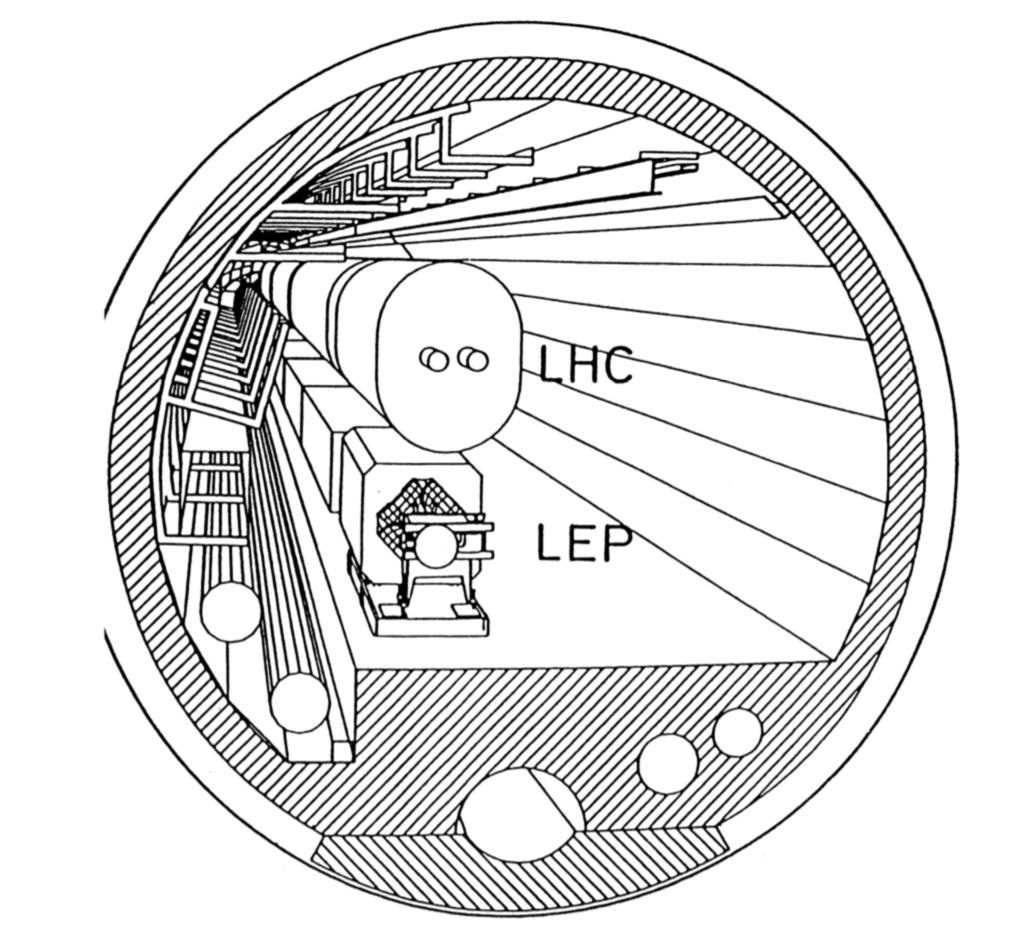
\includegraphics[width=0.43\textwidth]{figures/chapter2/lhc_lep_dipole_comp}
        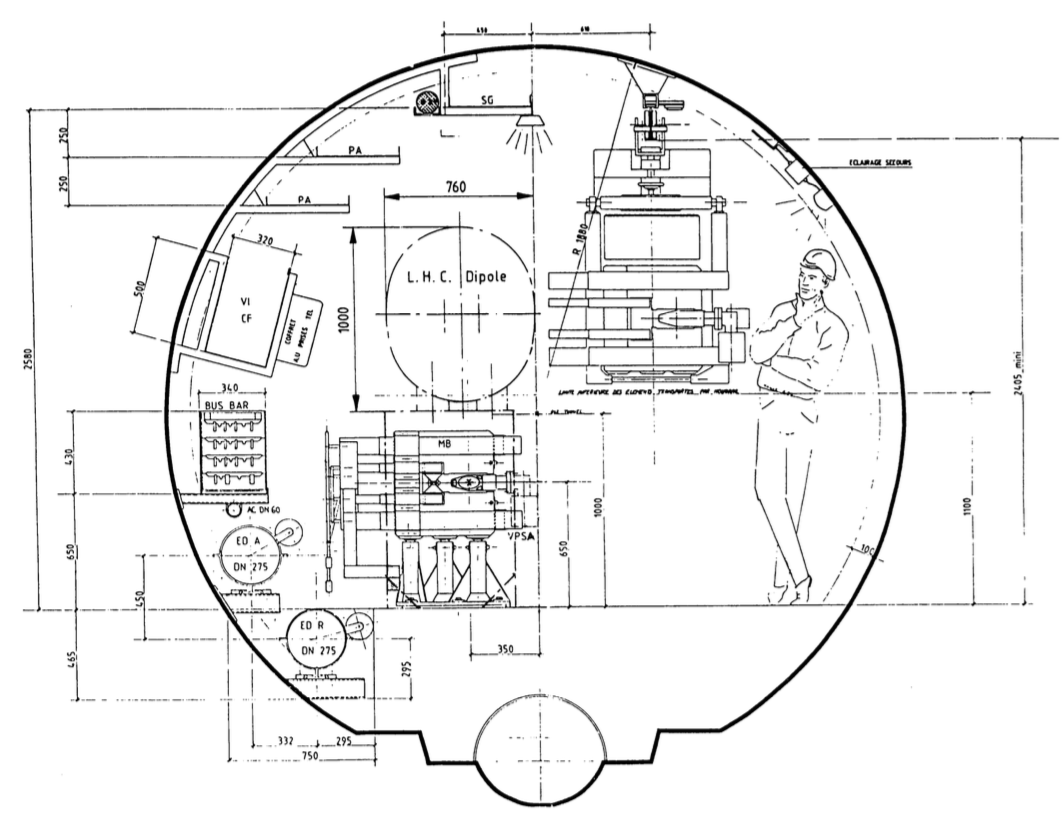
\includegraphics[width=0.50\textwidth]{figures/chapter2/lhc_lep_dipole_comp_person}
        \caption{
            \textit{Left}: Illustration comparing the size of a `2-in-1' LHC dipole configuration to the
                LEP dipole and how they fit inside of the LEP/LHC tunnel. Note that prior to LHC operation,
                the LEP magnets will have been removed: the two are shown side-by-side for comparison purposes only.
            \textit{Right}: Cross-sectional view of the LEP/LHC tunnel with a comparison of the LHC `2-in-1' dipole
                on top of the LEP dipole. An illustration of an average size person is shown
                for scale. Also shown is the service crane in use, to give an idea of the size required
                for potential maintenance access. Clearly, two single-bore, superconducting rings each similar in size
                to the LEP dipole would not fit comfortably in the tunnel. The LHC `2-in-1' design fits
                in nearly the same area as the LEP dipoles while additionally being able to contain both
                particle beams.
                Figures are taken from Ref.~\cite{ECFALHCinLEP}.
        }
        \label{fig:lhc_lep_dipole_comp}
    \end{center}
\end{figure}

\begin{figure}[!htb]
    \begin{center}
        \begin{minipage}{\textwidth}
        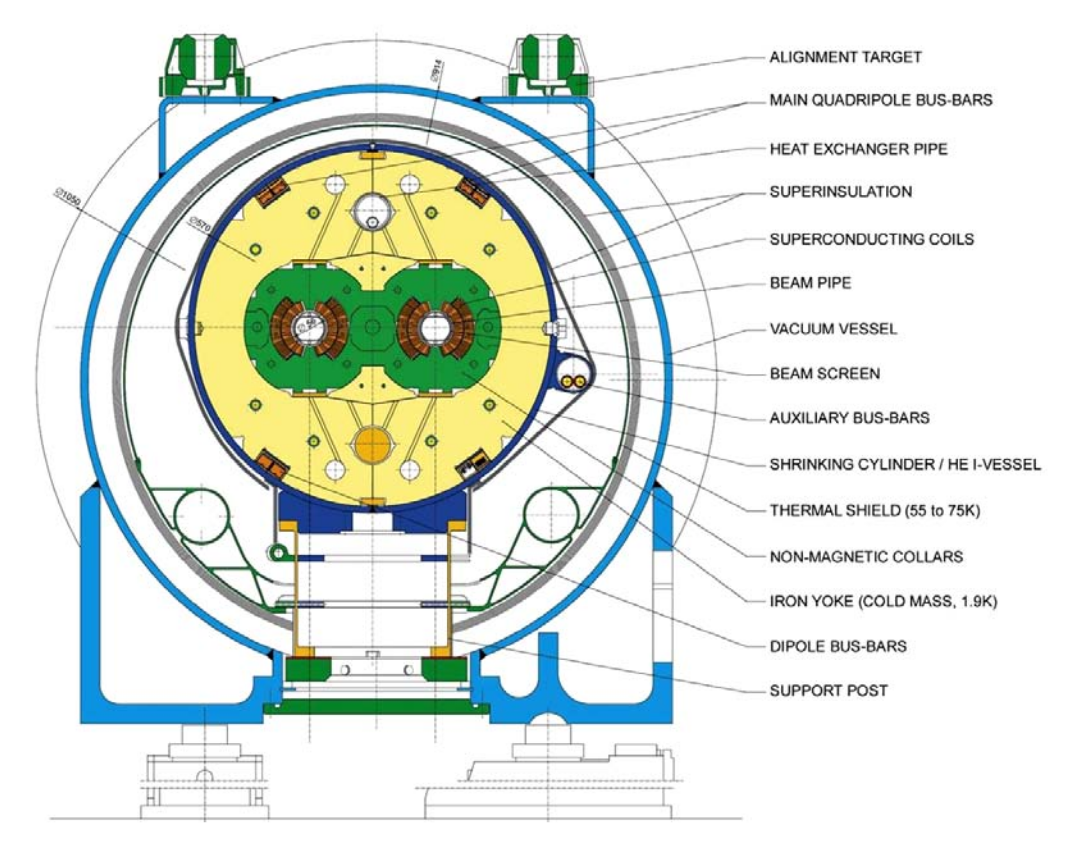
\includegraphics[width=0.59\textwidth]{figures/chapter2/lhc_dipole_fig3p3}
        \raisebox{0.5cm}{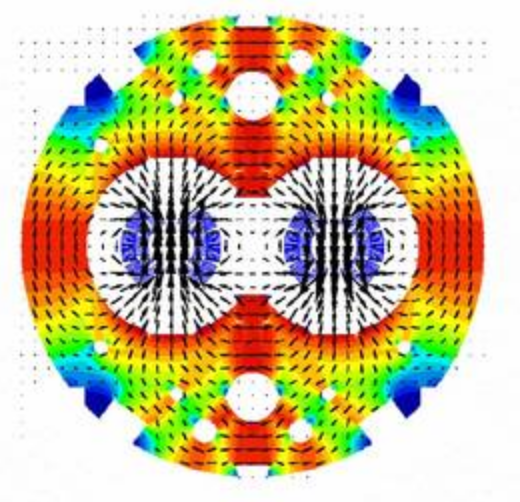
\includegraphics[width=0.4\textwidth]{figures/chapter2/dipole_magnetic_field_lines}}
        \end{minipage}
        \caption{
            \textit{Left}: Cross-sectional view of an LHC dipole bending magnet, with relevant parts indicated.
            The protons orbit inside of the beam pipes, each of which has a diameter of roughly $3$\,cm.
            It is interesting to note that the non-magnetic steel collars (in green) are of critical import
            to the success of the magnet systems. They are required
            to prevent the dipole structure from being deformed or torn apart due to the intense magnetic forces
            tending to push the two beam-pipes apart as a result of their counter-rotating electromagnetic currents.
            These forces amount to about 400 tonnes per meter of dipole when in full operation --- almost equivalent in magnitude
            to the weight of a Boeing 747.
            \textit{Right}: Magnetic field lines of the coupled dipole fields that bend the counter-rotating proton beams
            and keep them in their circular orbits around the LHC ring.
        }
        \label{fig:lhc_dipole_xsec}
    \end{center}
\end{figure}


%\FloatBarrier
\paragraph{Connecting the Dots} \mbox{} \\
The LHC is essentially a chain of superconducting magnets of the type described in the previous paragraphs, where
the the bending (dipole) magnets critical to the LHC design were introduced.
%There are additional
%types of magnets that produce fields of higher multipole moments which, in the case of the quadrupole magnets, are
%necessary for beam \textit{beam focusing}. Conceptually they are very similar to the dipoles and are 
The chain is laid in a double-octagonal structure, illustrated in Figure~\ref{fig:lhc_layout}. There are eight
octants, at the center of which the LHC ring is straight and does not curve.
The LHC curvature occurs at the
boundaries of each of the octants and is primarily made up of bending (dipole) magnets.
The straight sections are where the interaction regions are located and are referred
to as `Points', numbered 1 to 8.
Points 1, 2, 5, and 8 are where the four large LHC experiments are located.
Points 1 and 5 are home to the services and underground areas
of the general purpose experiments, ATLAS and CMS, respectively.
The underground experimental caverns associated with Point 1 and 5 were not present for LEP and
had to be constructed after LEP was retired in 2000.
Figure~\ref{fig:p1} provides an illustration of how the surface and underground
areas are situated at Point 1.
Points 2 and 8 host the services and underground areas of the ALICE and LHCb experiments, respectively.
At these Points, Points 1, 2, 5, and 8, the counter-rotating beams are
made to collide. The remaining Points, Points 3, 4, 6, and 7, are host to various beam `services'
necessary for the operation of the LHC.
Point 3 and 7 host the beam betatron and momentum cleaning (`beam collimation') systems, respectively.
Point 4 hosts the superconducting radio-frequency (RF) systems which accelerate the beams to
their nominal collision energies.
Point 6 is the location of the beam-abort system --- the so-called `beam dump' --- where
the LHC beams may be removed very quickly from the LHC ring by using \textit{kicker} magnets~\cite{LHCDesignI}
that divert the beams out of the LHC ring in a safe manner. The beams may be dumped
if the LHC wishes to refill with protons (or heavy-ions) and needs to remove any
remnants of the previous fill, in case of beam instabilities observed in the LHC ring,
or if one of the experiments signals the need for a beam dump (in case of
beam stability or detector issues observed at the associated IP).

\begin{figure}[!htb]
    \begin{center}
        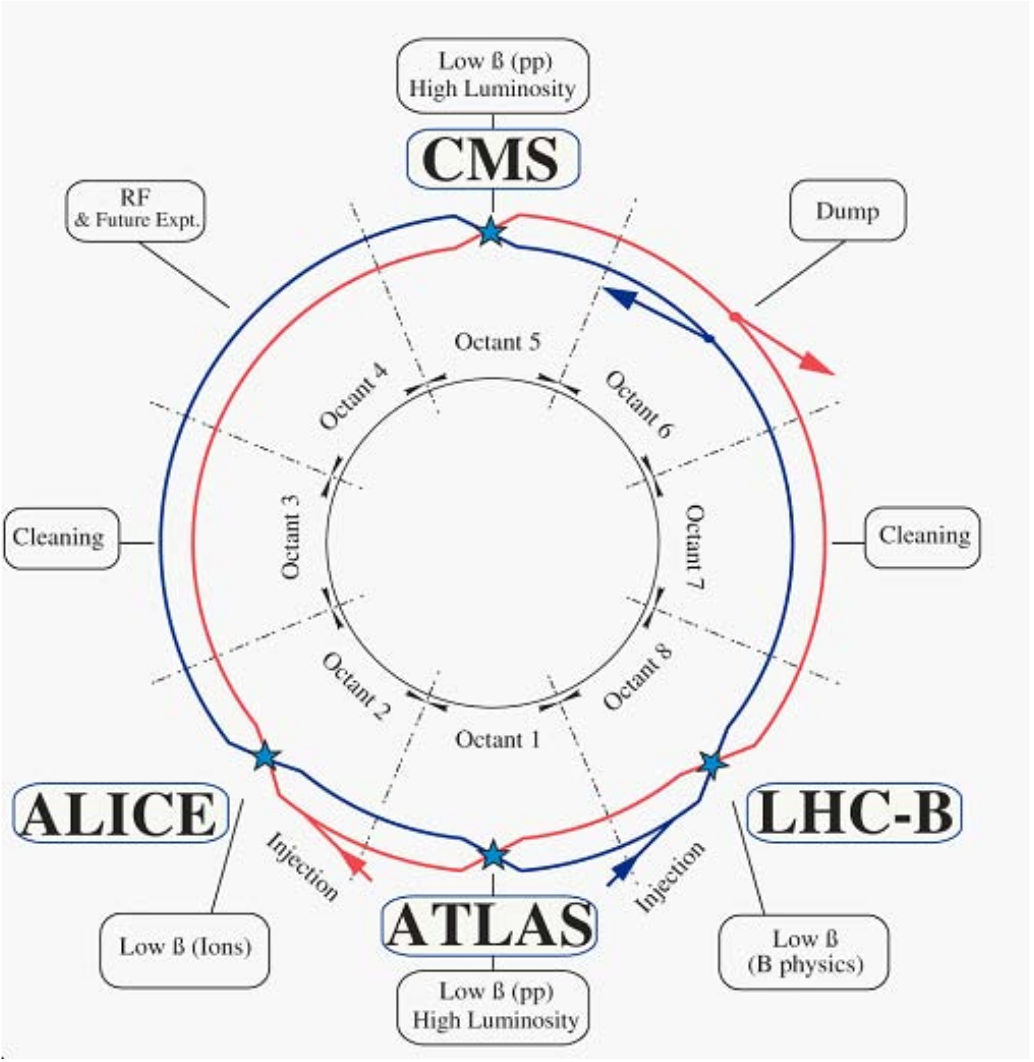
\includegraphics[width=0.8\textwidth]{figures/chapter2/lhc_layout}
        \caption{
            Layout of the LHC and its two counter-rotating beams. Beam 1 is in blue and rotates
            counter-clockwise. Beam 2 is in red and rotates clock-wise.
            At the center of each octant is a straight section which houses
            the experimental caverns or LHC beam facilities.
            At the boundaries of each octant are located the curved sections.
            Figure taken from Figure 2.1 of Ref.~\cite{LHCMachine}.
            {\color{red}{Somewhere $\beta$ should be described -- betatron function}}
        }
        \label{fig:lhc_layout}
    \end{center}
\end{figure}

\begin{figure}[!htb]
    \begin{center}
        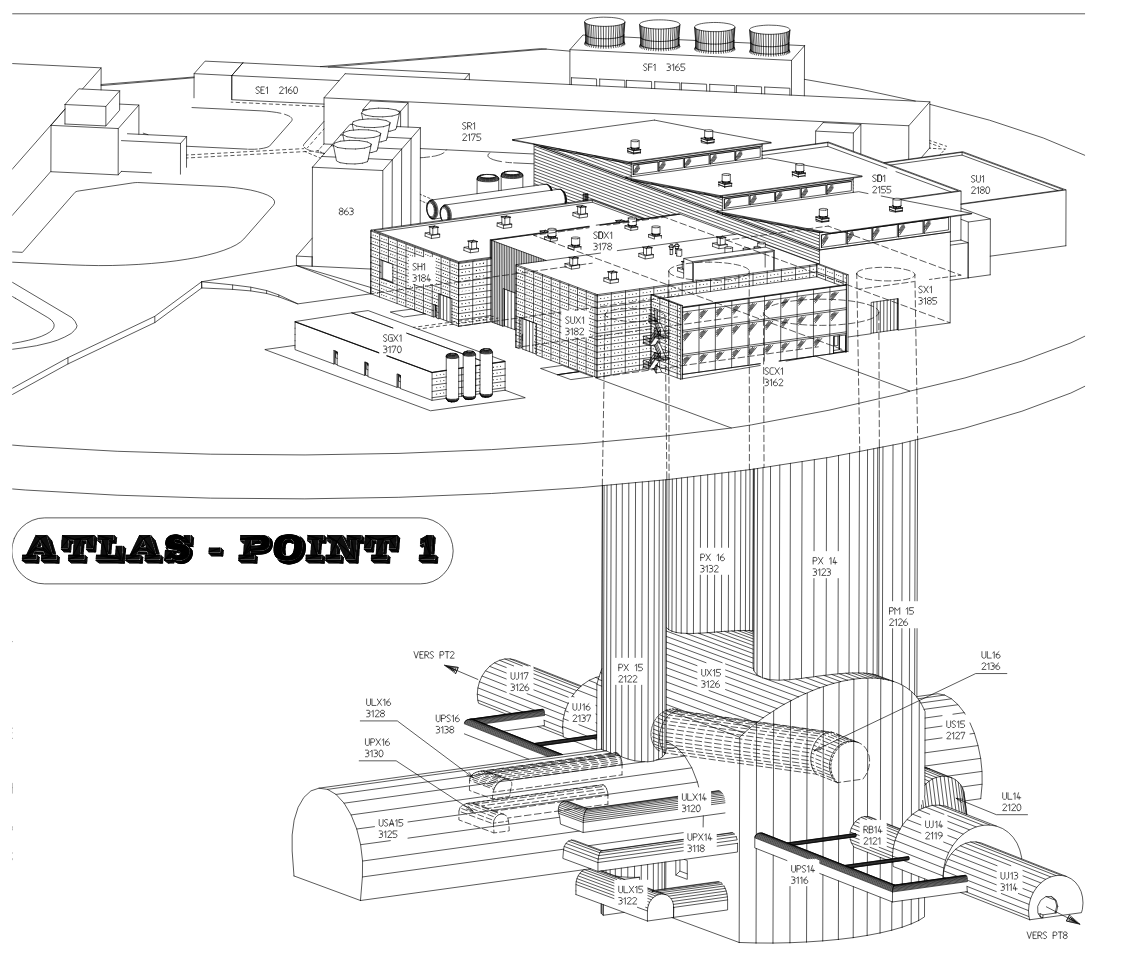
\includegraphics[width=0.75\textwidth]{figures/chapter2/point1_illustration}
        \caption{
            Diagram showing the surface buildings and services and underground areas of Point 1, where
            the ATLAS experiment is located. The LHC ring can be seen at the bottom,
            with its directions indicated by the `VERS PT8 (2)' arrows pointing
            towards Point 8 (2).
            The experimental cavern in which the ATLAS detector sits is UX15.
            The control room for the ATLAS experiment, whereat operators can monitor and
            control the state of the ATLAS detector, is located 100\,m above
            UX15 in the building SCX1.
            Figure taken from Figure 10.1 of Ref.~\cite{LHCDesignII}.
        }
        \label{fig:p1}
    \end{center}
\end{figure}

%\FloatBarrier
\subsection{Injection Chain and Bunch Structure}
\label{sec:lhc_injection}

We now have an idea of how the proton beams relevant to the work
in this thesis are made to circulate in the LHC ring.
In this section we will briefly describe the initial source of the protons and how
they are introduced into the LHC ring.
The LHC relies on a series of pre-acceleration steps that bring the initial
low-energy protons to energies sufficient enough to begin their journey through the LHC.
The sum-total of these steps is referred to as the LHC \textit{injection chain}~\cite{LHCDesignIII}.
The components of the LHC injection chain form the heart of the CERN accelerator
complex illustrated in Figure~\ref{fig:cern_complex}.
For $pp$ collisions in the LHC, the protons are initially sourced from Hydrogen atoms that are released
at the start of Linac 2.
The Hydrogen atoms are immediately stripped of their electrons after passing through
the \textit{duoplasmatron} ion source~\cite{Duoplasma}.
The protons are then passed through Linac 2, a linear accelerator, which accelerates
the protons to $50$\,\MeV.
They then enter the Proton Synchotron Booster (PSB), a circular storage ring
composed of four stacked rings, which accelerates the protons to $1.4\,\GeV$.
The PSB injects the protons into the Proton Synchotron (PS) which accelerates
them to $25$\,\GeV.
The Super Proton Synchotron (SPS) receives the protons from the PS and
accelerates them to $450$\,\GeV.
At this point the protons have sufficient energy to be injected into the LHC.
There are two injection points into the LHC since, up until this stage,
the protons are circulating in the same direction: one injection point sends
protons into the counter-clockwise beamline of the LHC, and the other
into the clockwise beamline.
Until all of the protons from a single \textit{fill} make their way into
the LHC, they will circulate at the injection energy of $450$\,\GeV.
After the filling completes\footnote{A standard LHC fill takes on the order of 4 minutes per
ring.}, the superconducting RF cavities located at Point 4 will begin to accelerate the protons
to their final collision energies.\footnote{If all goes smoothly, this acceleration stage takes roughly 20 minutes.}
The acceleration is achieved by increasing the frequency of the RF oscillations; however,
given that a $450$\,\GeV~proton is already ultra-relativistic, the adjustment of the frequency
needed to get to the collision energies is not large.

The proton beams circulating the LHC are not a continuous stream of protons; rather,
they are grouped into what are referred to as \textit{bunches}.
The protons arrive at the LHC in these bunches which are initially prepared
in the smaller machines that make up the LHC injection chain and then are
kept in their final \textit{bunch structure} by the RF cavities.
The accelerating RF cavities provide an accelerating electromagnetic field
that oscillates longitudinally. The bunches, each composed of roughly $10^{11}$ protons,
are then made to oscillate longitudinally in so-called \textit{synchotron oscillations}
around the central node of the RF oscillation as they circulate through the LHC ring.
The proton bunches are then effectively `shaped' by the oscillating RF field: protons in a bunch
lagging behind or that are ahead of those particles at the center of the bunches
will be accelerated or decelerated accordingly so as to be pushed back into the center of the bunch.
The LHC RF cavities have an oscillation frequency of $400$\,MHz which
defines the boundaries in which proton bunches can lie. These boundaries are
called \textit{RF buckets} and, along with
the circumference of the LHC, dictate the number of proton bunches that
can potentially fit in the LHC.
The relationship between the RF oscillations and the RF bucket and bunch structure
is illustrated in Figure~\ref{fig:lhc_bunch}.
In total, approximately 35640 RF buckets exist when the LHC is in operation.
Not all buckets contain proton bunches, however.
In fact, at the time of the writing of the present thesis,
RF buckets filled with proton bunches have a minimal separation of 10 RF buckets, meaning
that following an RF bucket containing a proton bunch there is at least 9 unfilled RF buckets.
This corresponds to a minimal
time between proton bunches --- the \textit{bunch spacing} --- of $25$\,nanoseconds.
At the time of the present thesis, the operating conditions of the LHC maximally
allow for 2808 $25$\,ns-spaced bunches.\footnote{
The number of allowed bunches is significantly lower than the 35640 RF buckets with $25$\,ns
bunch-spacing potentially allow for. This is due, in part, to the non-trivial bunch-structure
typically employed but also in large part to the fact that there is a rather long \textit{abort gap}
in the LHC ring where no filled RF buckets exist.
The abort gap is a number of continuous unfilled RF buckets that allows the ramp up of the kicker
magnets used for the beam dump to occur in the absence of filled buckets.
In this way, the kicker magnet ramp up does not disturb the structure of the circulating proton beams.
Only after this ramp up is finished should the kicker magnets disturb the beams.
}
The bunch-spacing and overall bunch structure of an LHC fill is not only decided
by the operators of the LHC but also by what the detectors at Points 1,2,5, and 8
can tolerate. This is because shorter bunch spacing means higher intensity and multiplicity
of collisions occuring at each of these IP. A $25$\,nanosecond bunch spacing
corresponds to a maximal $pp$ collision rate of $40$\,MHz. The detectors at each
of the IP have been designed with this collision rate in mind and anything
higher may push them beyond their design limits.

\begin{figure}[!htb]
    \begin{center}
        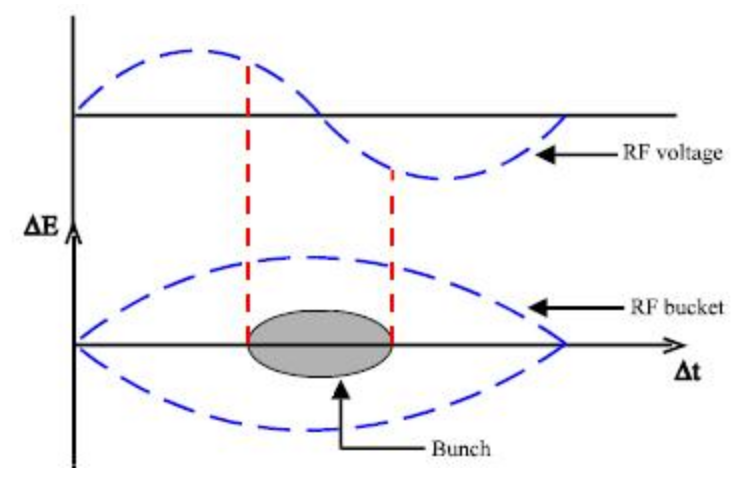
\includegraphics[width=0.5\textwidth]{figures/chapter2/lhc_bunch}
        \caption{
            Illustration of the particle bunch structure in a particle collider such as the LHC.
            The particles are accelerated by radio-frequency (RF) oscillations whose
            amplitude is illustrated in the upper plot.
            The RF bucket's boundary, illustrated in the lower plot, is defined by a full period of the RF oscillation
            and the particle bunch formation, depicted in grey, occurs at the central node of the oscillation.
            The area occupied by the particle bunch is related to the beam's longitudinal
            \textit{emittance}.
        }
        \label{fig:lhc_bunch}
    \end{center}
\end{figure}

\subsection{The Concept of Luminosity}
\label{sec:lhc_luminosity}

In designing a particle collider, the collision energy is not the only important parameter.
Equally important is the value of the instantaneous \textit{luminosity}
that can be achieved by the collider.
An expression for the instantaneous luminosity, $\mathcal{L}$, is given by,
\begin{align}
    \mathcal{L} = \frac{N^2 n_b f}{4 \pi \sigma_x \sigma_y} \cdot S,
    \label{eq:luminosity}
\end{align}
where $N$ is the number of particles per bunch, $n_b$ is the number of colliding bunches,
$f$ is the bunch revolution frequency, $\sigma_{x,y}$ are the transverse beam widths in the
Gaussian approximation, and $S$ is a reduction factor that accounts for geometric factors
such as the non-zero crossing-angle of the colliding beams~\cite{LHCDesignIII,LumiConcept}.
The instantaneous luminosity, $\mathcal{L}$, can be seen by Eqn.~\ref{eq:luminosity}
to have units of cm$^{-2}$s$^{-1}$ and can be conceptually thought of as the
outgoing flux of particles per unit area and time after a bunch crossing in which successful $pp$
collisions occur.
The LHC is designed to deliver collisions to the high luminosity IP (Fig.~\ref{fig:lhc_layout})
at $\mathcal{L} = 10^{34}$\,cm$^{-2}$s$^{-1}$.
Accurate knowledge of $\mathcal{L}$ is of the utmost importance for collider design and operation.
Not only does it parametrise the potential collision rate once the collider beam and bunch
structure are decided, but it allows for the accurate prediction of the number
of collision events, $N_{\text{proc}}$, associated with a particular physics process
with cross-section $\sigma_{\text{proc}}$,
\begin{align}
    N_{\text{proc}} = \sigma_{\text{proc}} \int \mathcal{L}\, \mathrm{d}t \equiv \sigma_{\text{proc}} \cdot L,
    \label{eq:n_exp_lumi}
\end{align}
where $L$ is referred to as the \textit{integrated luminosity} and has units of cm$^{-2}$.
A common unit for integrated luminosity is the \textit{barn}, with symbol `b': one barn is defined as $10^{-24}$\,cm$^{-2}$.
The datasets collected by the LHC experiments are such that the \textit{femtobarn} (fb), $10^{-39}$\,cm$^{-2}$, is relevant.

\subsection{Operation of the Large Hadron Collider}
\label{sec:lhc_operation}

The LHC has been in stable operation since 2009.
It operates in so-called \textit{runs}: multi-year periods of roughly continuous
data-taking.
As CERN shuts down during the winter months, each run is segmented each year
with a several month long shutdown in the winter with a ramp-up period in the spring.
During these shorter shutdowns, maintenance and upgrades may also take place.
In between a given run there is a multi-year break, a \textit{long shutdown},
in which large(er)-scale maintenance and upgrades of both the LHC and the experiments can take place.
At the time of writing, there has so far been two runs of the LHC, Run-I and Run-II.
Run-I took place during the years 2009--2012 and Run-II during 2015--2018.
The integrated luminosities for each of the data taking years between Run-I and Run-II
is shown in Fig.~\ref{fig:int_lumi_multiyear}.
The data relevant to the work presented in this thesis were collected in both
Run-I and Run-II of the LHC, specifically that data collected in the years 2012--2018.
The luminosities, instantaneous and integrated, as well as the center-of-mass collision energies, $\sqrt{s}$, for these data-taking periods are
shown in Table~\ref{tab:lumi_tab}.
Also shown in Table~\ref{tab:lumi_tab} are the average values of the mean number of interactions per bunch
crossing, $\langle \mu \rangle$, observed during each data-taking year. The quantity $\langle \mu \rangle$
is related to the amount of \textit{pileup} observed during data-taking. Pileup is caused
by overlapping $pp$ interactions within the same (\textit{in-time} pileup) or neighboring (\textit{out-of-time} pileup)
bunch-crossing(s) at the interaction point. The pileup scales with the instantaneous luminosity.
Distributions of $\langle \mu \rangle$ are shown in Fig.~\ref{fig:int_lumi_multiyear} for
the Run-II data-taking period.


\begin{table}[!htb]
    \begin{center}
        \begin{tabular}{l | c | c c c c }
        \hline
        \hline
        & \textbf{Run-I} & \multicolumn{4}{c}{\textbf{Run-II}} \\
        \hline
        Year & 2012 & 2015 & 2016 & 2017 & 2018 \\
        \hline
        Collision energy, $\sqrt{s}$ [TeV] & 8 & \multicolumn{4}{c}{13} \\
        Peak Luminosity, $\mathcal{L}$ [cm$^{-2}$s$^{-1}$] ($\times10^{34}$) & $0.77$ & $0.5$ & $1.4$ & $2.1$ & $2.1$ \\ 
        Integrated Luminosity, $L$ [fb$^{-1}$] & 20.2 & 3.2 & 33.0 & 44.3 & 59.9 \\
        Mean number of of interactions & & & & & \\
        \hspace{1.7cm} per bunch crossing, $\langle \mu \rangle$ & 20.7 & 13.4 & 25.1 & 37.8 & 36.1 \\
        \hline
        \hline
        \end{tabular}
        \caption{
            Summary parameters for the data-taking periods relevant to the work
            presented in this thesis. The integrated luminosity is that relevant
            to performing physics analysis and potentially differs with respect to
            the total integrated luminosity delivered to ATLAS by the LHC (Fig.~\ref{fig:int_lumi_multiyear}) due to
            the application of strict quality criteria on the data prior to its use
            in physics analyses.
        }
        \label{tab:lumi_tab}
    \end{center}
\end{table}

\begin{figure}[!htb]
    \begin{center}
        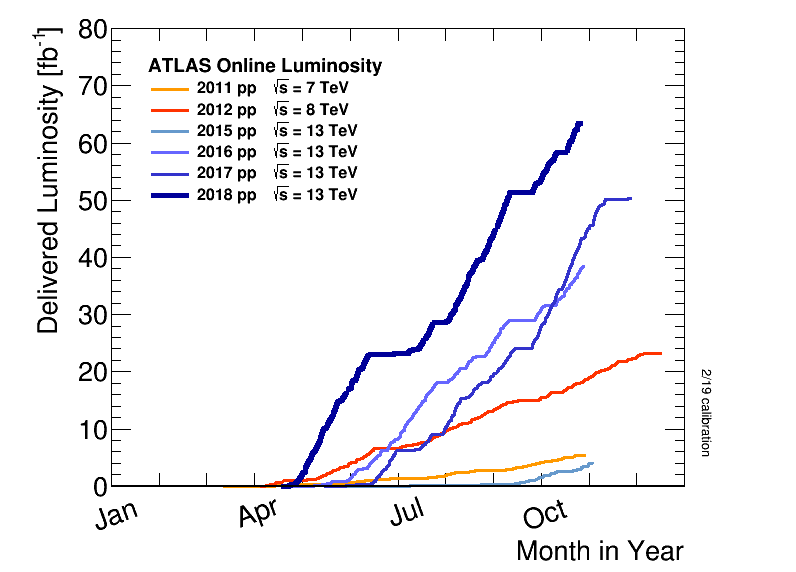
\includegraphics[width=0.49\textwidth]{figures/chapter2/int_lumi_multiyear}
        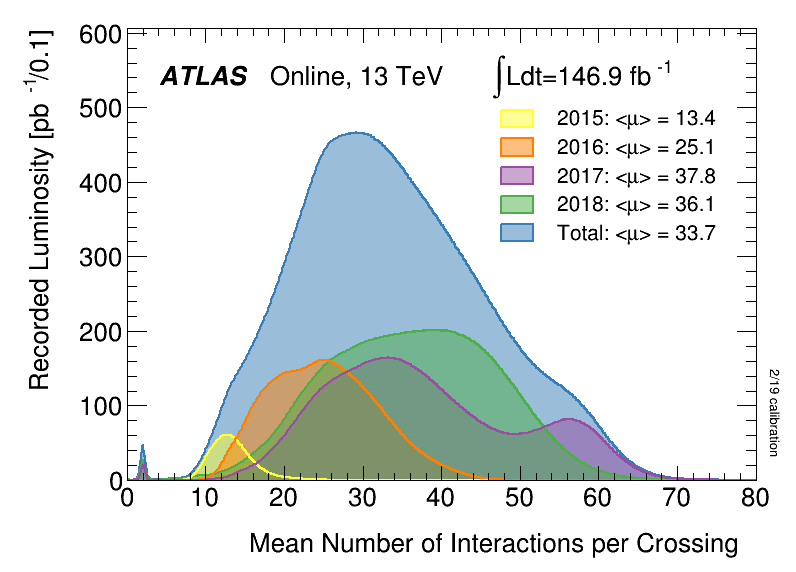
\includegraphics[width=0.49\textwidth]{figures/chapter2/mu_run2}
        \caption{
            \textit{Left}: The ATLAS integrated luminosity during the data-taking years 2011--2018.
            \textit{Right}: The observed average number of $pp$ interactions per bunch-crossing, $\langle \mu \rangle$,
                observed by ATLAS during the Run-II data-taking years, 2015--2018.
        }
        \label{fig:int_lumi_multiyear}
    \end{center}
\end{figure}


%%%%%%%%%%%%%%%%%%%%%%%%%%%%%%%%%%%%%%%%%%%%%%%%%%%%%%%%%%%%%%%%%%%
%%%%%%%%%%%%%%%%%%%%%%%%%%%%%%%%%%%%%%%%%%%%%%%%%%%%%%%%%%%%%%%%%%%
% sub-section describing ATLAS
%%%%%%%%%%%%%%%%%%%%%%%%%%%%%%%%%%%%%%%%%%%%%%%%%%%%%%%%%%%%%%%%%%%
%%%%%%%%%%%%%%%%%%%%%%%%%%%%%%%%%%%%%%%%%%%%%%%%%%%%%%%%%%%%%%%%%%%
\section{The ATLAS Detector}
\label{sec:atlas}

In this section we will extend our focus to the ATLAS detector, the general purpose
particle detector located at Point 1 of the LHC ring (see Figure~\ref{fig:p1}).
Roughly cylindrical in shape, coaxial with the beam-pipe,
the ATLAS detector is 44\,m long and 25\,m tall.
It is by far the largest such detector ever built and,
generally, is the largest and most complex device ever constructed.
Being general purpose in scope, the ATLAS detector is hermetic and has
nearly $4\pi$ radians of solid angle coverage around the $pp$ collision
point. 
Such detectors are commonly designed to have various subsystems --- \textit{subdetectors} ---
which are designed for the identification of specific types of particles
and interactions.
They tend to be layered about the interaction point and cylindrically symmetric
since the $pp$ interactions taking place within the detector have no preferred
direction in the plane transverse to the direction in which the proton beams
are travelling.
A view of the ATLAS detector and its subdectors is provided by Figure~\ref{fig:atlas_cutaway}.
In the following we will briefly describe each subsystem in turn, describing
first the detectors located nearer to the $pp$ collision and proceeding outwards.

\subsection{The ATLAS Coordinate System}
\label{sec:atlas_coordinate_system}

The ATLAS detector uses a right-handed coordinate system with the origin located at
the geometric center of the detector.
The $x$-axis points to the center of the LHC ring, the $y$-axis points upwards
and away from the center of the Earth, and the $z$-axis is along the beam-pipe.
The side associated with positive (negative) $z$
is referred to as the `A' (`C') side of the detector.\footnote{`A' for `airport',
since this is the side pointing towards Geneva International Airport, and
`C' for either `Crozet' or `Charly's', depending on who you ask, since this is the side
pointing towards the town of Crozet and/or Charly's Pub in the town of Saint-Genis-Pouilly.}
Due to its cylindrical symmetry, ATLAS also uses the cylindrical coordinates, $(r,\phi, z)$,
with $\phi$ the azimuthal angle about the $z$-axis and having $\phi = 0$ along the positve $x$-axis.
The spherical polar angle, $\theta$, is defined with respect to the $z$-axis, having
$\theta = 0$ parallel to the beam-pipe and $\theta = \pi/2$ in the $xy$-plane transverse
to the beam-pipe.
The pseudorapidity, $\eta$, is commonly used when describing systems of particles or locations within
the detector and is defined as $\eta = - \ln \left[ \tan \left( \theta / 2 \right) \right ]$.
The relationship between pseudorapidity and polar angle is illustrated in Figure~\ref{fig:eta_desc}.
Large (small) values of $\eta$ correspond to the \textit{forward} (\textit{central}) region of the detector.
The rapidity, $y$, is related to $\eta$ and is defined as $y = \frac{1}{2} \ln \left[ (E+p_z) / (E-p_z) \right]$.
The pseudorapidity of a particle traversing the detector is equal to its rapidity if
the particle is massless or ultra-relativistic; otherwise, they are different.
The comparison between a particle's pseudorapidity and rapidity is illustrated in
Figure~\ref{fig:eta_desc}.
The coordinates used to describe systems of particles are typically described by their
four-momenta: $(p_x, p_y, p_z)$ or, equivalently, $(\pT, \eta, \phi)$.
A distance metric commonly used to describe the distance between two systems of particles
in the detector is $\Delta R = \sqrt{ (\Delta \eta)^2 + (\Delta \phi)^2 }$. The
$\Delta R$ quantity using $y$ instead of $\eta$ is also sometimes used and will be
indicated by $\Delta R_y$.

\begin{figure}[!htb]
    \begin{center}
        \raisebox{1.5cm}{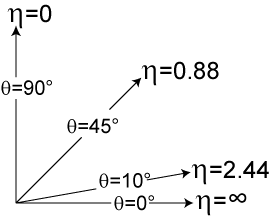
\includegraphics[width=0.35\textwidth]{figures/chapter2/eta_vs_polar}}
        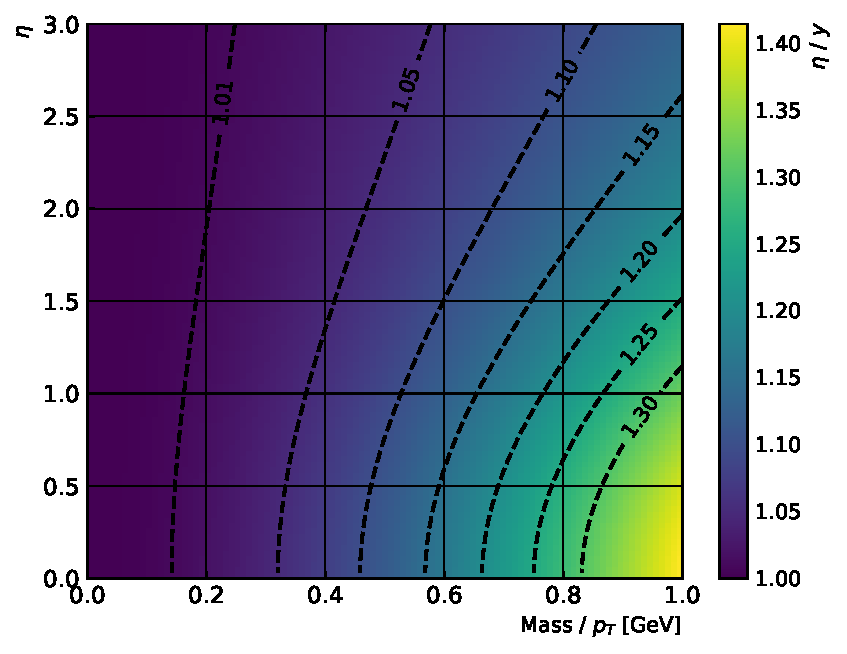
\includegraphics[width=0.55\textwidth]{figures/chapter2/eta_vs_rap}
        \caption{
            \textit{Left}: Illustration of the relationship between the pseudorapidity, $\eta$,
                and polar angle, $\theta$, defined as the angle with respect to the beam-axis ($z$-axis).
            \textit{Right}: Distribution of the ratio of a particle's pseudorapidity to its rapidity, $\eta$/$y$,
                as a function of its pseudorapidity ($y$-axis) and the ratio of its mass to its transverse momentum, \pT~($x$-axis).
        }
        \label{fig:eta_desc}
    \end{center}
\end{figure}


\begin{figure}[!htb]
    \begin{center}
        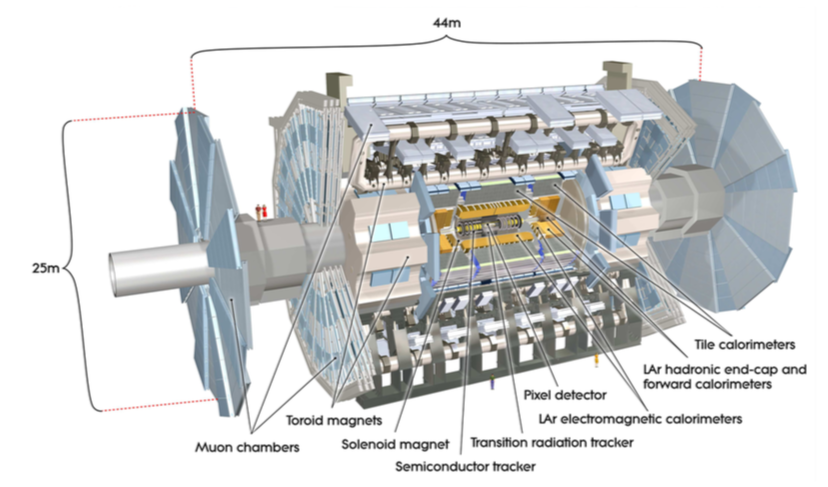
\includegraphics[width=0.95\textwidth]{figures/chapter2/atlas_cutaway}
        \caption{
            Cut-away view of the ATLAS detector with sub-systems indicated.
            Shown for comparison are figures of average-height humans standing
            at the feet of the detector and standing on the forward shielding
            between the big wheels of the forward muon system.
        }
        \label{fig:atlas_cutaway}
    \end{center}
\end{figure}


\begin{figure}[!htb]
    \begin{center}
        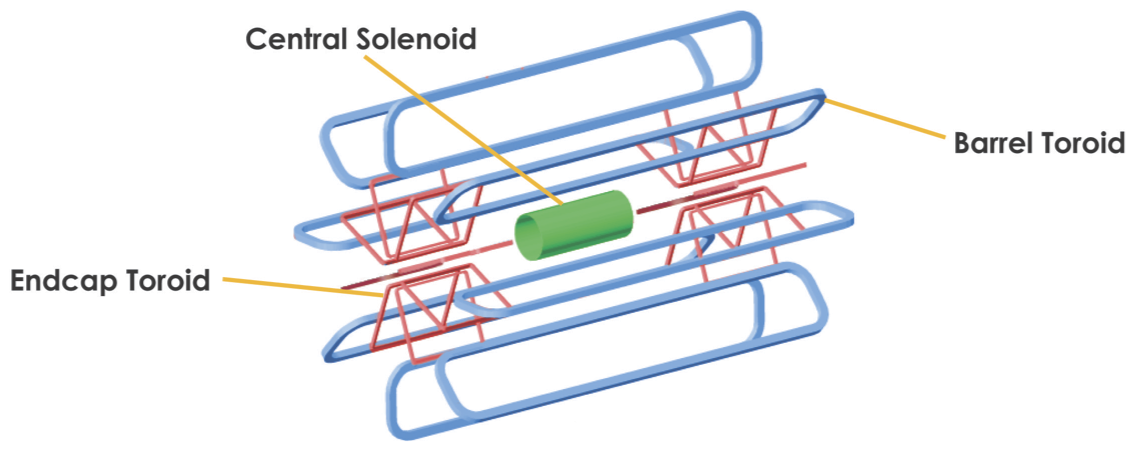
\includegraphics[width=0.95\textwidth]{figures/chapter2/atlas_magnet_system}
        \caption{
            A view of the ATLAS magnet system. Shown are the 2\,T solenoid magnet
            in green, the barrel toroid system in blue, and endcap toroid magnets
            in red.
        }
        \label{fig:atlas_magnet_system}
    \end{center}
\end{figure}

%%%%%%%%%%%%%%%%%%%%%%%%%%%%%%%%%%%%%%%%%%%%%%%%%%%%%%%%%%%%%%%%%%%%%
%%%%%%%%%%%%%%%%%%%%%%%%%%%%%%%%%%%%%%%%%%%%%%%%%%%%%%%%%%%%%%%%%%%%%
%
% INNER DETECTOR
%
%%%%%%%%%%%%%%%%%%%%%%%%%%%%%%%%%%%%%%%%%%%%%%%%%%%%%%%%%%%%%%%%%%%%%
%%%%%%%%%%%%%%%%%%%%%%%%%%%%%%%%%%%%%%%%%%%%%%%%%%%%%%%%%%%%%%%%%%%%%
\subsection{The Inner Detector}
\label{sec:inner_detector}

The innermost subdetector of ATLAS is the Inner Detector (ID)~\cite{Haywood:331064}.
The ID covers the region $\lvert \eta \rvert < 2.5$ and is composed, in order
of increasing radial distance from the beam-pipe, of the pixel detector,
semiconductor tracker (SCT), and the transition radiation tracker (TRT).
These detectors enable the reconstruction of the tracks associated with
the $\mathcal{O}(1000)$ charged particles emerging from each $pp$ bunch collision, occuring
every 25\,ns.
An illustration of the ID and its subdetectors is shown in Figure~\ref{fig:atlas_inner_detector}.
Additional, more detailed views of the barrel and endcap sections of the ID are shown in Figure~\ref{fig:atlas_ID_exploded}.
The ID is situated inside of the central solenoid, indicated in Figure~\ref{fig:atlas_magnet_system},
which provides an axial 2\,T magnetic field and extends over a length of 5.3\,m with a diameter of 2.5\,m.
The bending of charged particles in the $xy$-plane due to the presence of the solenoidal
field allows for their momenta to be measured using the curvature of their reconstructed tracks.

\begin{figure}[!htb]
    \begin{center}
        \includegraphics[width=0.75\textwidth]{figures/chapter2/atlas_inner_detector}
        \caption{
            Cross-sectional view of the ATLAS inner detector. Shown are the barrel
            and end-cap portions of the pixel, SCT, and TRT detectors.
        }
        \label{fig:atlas_inner_detector}
    \end{center}
\end{figure}

\begin{figure}[!htb]
    \begin{center}
        \includegraphics[width=0.6\textwidth]{figures/chapter2/atlas_ID_barrel_exploded}
        \raisebox{1.4cm}{\includegraphics[width=0.85\textwidth]{figures/chapter2/endcap_ID_exploded}}
        \caption{
            Exploded views of the barrel (\textit{left}) and endcap (\textit{right}) portions
            of the inner-detector.
        }
        \label{fig:atlas_ID_exploded}
    \end{center}
\end{figure}

\subsubsection{The Pixel Detector and IBL}
\label{sec:id_pixel}

The pixel detector is the innermost subdetector of the ID, situated very near to and surrounding
the beam-pipe.
It is composed of three separate sections: a barrel section and two end-cap sections.
The barrel section  of the pixel detector has a cylindrical geometry and the end-cap sections
are disks centered on the beam-pipe.
The barrel section has four layers, each with increasing radius, and there are three disks in each
of the end-caps. This ID geometry, shown in Figure~\ref{fig:atlas_ID_exploded}, covers
the region $\lvert \eta \rvert < 2.5$.

The pixel detector, being so near the $pp$ collisions, is subject to the highest particle
fluxes of any other subsystem.
As a result, it is built to have very fine granularity: its sensing elements consist of
$250$\,\micron~thick detectors housing pixels of reverse-biased n-type semiconductor material,
each having a nominal size of $50\times400\,\micron^2$.
In total, there are roughly 80 million channels read out from the pixel detector alone.
This allows for the pixel detector's fine spatial hit resolution of $10\,\micron$ in
$(r-\phi)$ and $115\,\micron$ along $z$.

The innermost layer of the pixel detector's barrel section is referred to as the
\textit{Insertable B-Layer} (IBL), and was installed at the beginning of the Run-II
data-taking period~\cite{Capeans:1291633}.
It corresponds, essentially, to the instrumentation of the ATLAS beam-pipe, as seen in Figure~\ref{fig:pixel_detector_trans},
and is located at a radial distance of 3.3\,cm.
It alone accounts for 8 million readout channels of
the pixel detector --- resulting in an ultra precise spatial hit resolution of $8\,\micron$ in $(r-\phi)$ and
$40\,\micron$ along $z$.
Beyond improving the overall measurements and reconstruction of charged particle tracks,
the IBL was installed in order to improve the performance of secondary vertex
reconstruction --- an essential ingredient to the algorithms associated with
the reconstruction and identification of jets originating from the decays
of $b$-hadrons whose decays occur at radial distances frequently beyond that
of the IBL.



\begin{figure}[!htb]
    \begin{center}
        \includegraphics[width=0.8\textwidth]{figures/chapter2/pixel_detector_trans}
        \caption{
            Transverse view of the barrel section of the pixel detector, showing
            the innermost layer, the Insertable B-Layer (IBL) (red), and the
            three surrounding layers (blue). From Ref.~\cite{Backhaus:2016ctq}.
        }
        \label{fig:pixel_detector_trans}
    \end{center}
\end{figure}


%%%%%%%%%%%%%%%%%%%%%%%%%%%%%%%%%%%%%%%%%%%%%%%%%%%%%%%%%%%%%%%%%%%%%
%%%%%%%%%%%%%%%%%%%%%%%%%%%%%%%%%%%%%%%%%%%%%%%%%%%%%%%%%%%%%%%%%%%%%
%
% CALORIMETERS
%
%%%%%%%%%%%%%%%%%%%%%%%%%%%%%%%%%%%%%%%%%%%%%%%%%%%%%%%%%%%%%%%%%%%%%
%%%%%%%%%%%%%%%%%%%%%%%%%%%%%%%%%%%%%%%%%%%%%%%%%%%%%%%%%%%%%%%%%%%%%
\subsection{Calorimeter Systems}
\label{sec:calorimeters}

The ATLAS calorimeter systems are situated outside of the ID and central solenoid and
are tasked with the measurement and containment of showers from electrically charged and neutral particles.
A view of the calorimeter systems is provided by Figure~\ref{fig:atlas_calorimeters_cutaway}.
Broadly speaking, there are two types of calorimeters based on their purpose:
electromagnetic and hadronic calorimeters.
The electromagnetic calorimeter system has $\eta$ coverage that matches the inner-detector
and is optimized for precision measurements of electrons and photons.
The hadronic calorimeter system has readout cells that are generally of
coarser granularity as compared to the electrogmagnetic calorimeter and
is designed to meet the requirements for jet and missing transverse momentum
measurements.
Besides classification by physics purpose, the calorimeter system can also
be broken into two classes based on detector technology: either based
on gaps of cooled liquid-argon~\cite{CERN-LHCC-96-041} or on scintillating tiles as the active media~\cite{CERN-LHCC-96-042}.

\begin{figure}[!htb]
    \begin{center}
        \includegraphics[width=0.9\textwidth]{figures/chapter2/calorimeters/atlas_calorimeter_cutaway}
        \caption{
            Cut-away view of the ATLAS calorimeter system, with liquid-argon and sctintillating-tile
            subsystems indicated.
        }
        \label{fig:atlas_calorimeters_cutaway}
    \end{center}
\end{figure}

\subsubsection{Electromagnetic Calorimeter}
\label{sec:calo_em}

The electromagnetic (EM) calorimeter is a high-granularity lead/liquid-argon (LAr)
sampling calorimeter situated outside of the ID and sharing the
same cryostat as the the central solenoid.
It consists of barrel and end-cap sections that cover the entire
range within $\lvert \eta \rvert < 3.2$ and is illustrated in Figure~\ref{fig:atlas_calorimeters_cutaway}.
The structures of the electromagnetic barrel and end-cap calorimeters
are shown in Figure~\ref{fig:em_calo_section}.
The EM calorimeter is designed in an accordian type structure to provide full coverage
in $\phi$.
The cooled LAr fills the gaps between layers of the
accordian structure.
Passing particles from the interaction point undergo scattering and bremsstrahlung processes as they pass through
the lead absorbers. The resulting electrons and photons ionise the LAr, producing
drift electrons and ions whose signals are read out by the interleaved readout
electrodes. The 2.1\,mm drift gap has an operating voltage of $\approx 2$\,kV.
The electromagnetic calorimeter is $>22$ radiation lengths ($X_0$), ensuring
that the majority of electrons and photons are completely contained within the EM calorimeter.
The majority of the EM energy, amounting to approximately 16\,$X_0$, is contained
within the second sampling layer (see Figure~\ref{fig:em_calo_section}).
The fine granularity of the readout, indicated in Figure~\ref{fig:em_calo_section},
was designed with the ability to distinguish individual photons arising from $\pi^0 \rightarrow \gamma \gamma$
decays. The ability to distinguish photons pairs so precisely is also important for the
main Higgs boson decay channel used for its disovery, $h \rightarrow \gamma \gamma$.

In the region $\lvert \eta \rvert < 1.8$, a so-called \textit{presampler} detector is used to correct
for the energy lost by electrons and photons due to material interactions occuring
upstream of the EM calorimeter.
It is a single LAr layer, with width 1.1\,cm (0.5\,cm) in the barrel (end-cap).

\begin{figure}[!htb]
    \begin{center}
        \includegraphics[width=0.6\textwidth]{figures/chapter2/calorimeters/atlas_em_calo_barrel}
        \raisebox{1.5cm}{\includegraphics[width=0.3\textwidth]{figures/chapter2/calorimeters/atlas_em_calo_endcap}}
        \caption{
            \textbf{\textit{Left}}: Cut-away view of the barrel electromagnetic calorimeter and its accordian
                structure. Indicated are
                the geometry and absorption properties of the three sampling layers.
                Also indicated is the granularity of the electrode readout in $\Delta \phi \times \Delta \eta$
                in each layer.
            \textbf{\textit{Right}}: Diagram of the electromagnetic end-cap calorimeter accordian wheel structure
                (only a sub-set of the accordian structure is shown).
        }
        \label{fig:em_calo_section}
    \end{center}
\end{figure}

\FloatBarrier
\subsubsection{Hadronic Calorimeter}
\label{sec:calo_had}

The barrel section of the hadronic calorimeter is composed of a
lead/scintillating-tile type detector whereas the end-cap hadronic
calorimeter is based on copper/LAr-based technology.

The lead/scintillating-tile calorimeter (the `tile calorimeter') is located just beyond
the EM calorimeter.
It is composed of a barrel section, covering $\lvert \eta \rvert < 1.0$,
and two extended barrels that cover $0.8 < \lvert \eta \rvert < 1.7$ (see Figure~\ref{fig:atlas_calorimeters_cutaway}).
It is a sampling calorimeter using steel as the passive absorber and scintillating
plastic tiles as the active media.
The tile calorimeter is composed of modules in which the scintillating
tiles are situated in $(r-\phi)$ within the steel absorbers, as shown in Figure~\ref{fig:tile_calo}.
The detector is segmented radially into three layers and the readout of the
scintillation light, using wavelength-shifting fibers that are fed into photomultiplier tubes (PMT)
situated along the outer radii, is organized in a projective
geometry, also illustrated in Figure~\ref{fig:tile_calo}.
In the barrel (extended barrel) section, most of the hadronic energy is captured by the first (last) two
layers which account for $\approx 5.5$ ($6$) hadronic interaction lengths ($\lambda$)
of the $\approx 7$ in total.

The hadronic end-cap (HEC) calorimeter consists of two wheels per end-cap, situated
behind the electromagnetic end-cap calorimeter, and
provides calorimetric coverage in the range $1.5 < \lvert \eta \rvert <3.2$.
A view of the HEC can be seen in Figures~\ref{fig:atlas_calorimeters_cutaway} and \ref{fig:fcal}.
The HEC calorimeter is built from layers of copper plates interleaved with 8.5\,mm LAr gaps
which provide the active medium for this sampling calorimeter.
The readout structure is obtained by dividing the gaps into separate drift zones for
which there are dedicated readout electrodes.
This readout structure is arranged in a projective geometry.

\begin{figure}[!htb]
    \begin{center}
        \includegraphics[width=0.4\textwidth]{figures/chapter2/calorimeters/atlas_tile_module}
        \includegraphics[width=0.9\textwidth]{figures/chapter2/calorimeters/atlas_tile_plan_view}
        \caption{
            \textbf{\textit{Top}}: A view of a tile calorimeter module with its interleaved steel
                absorbers and scintillating tiles and PMT readout. Also indicated are the source tubes
                through which radioactive Cesium (Cs) sources are passed for calibration purposes~\cite{Marjanovic:2018ohl}.
            \textbf{\textit{Bottom}}: Illustration of the segmentation of the projective readout of
                both the barrel and extended barrel tile calorimeter.
        }
        \label{fig:tile_calo}
    \end{center}
\end{figure}

\FloatBarrier
\subsubsection{Forward Calorimeter}
\label{sec:calo_forward}

The forward calorimeter (FCal) system~\cite{Artamonov_2008} provides calorimetric coverage to
high $\lvert \eta \rvert$, between $3.1 < \lvert \eta \rvert < 4.9$,
furthering the hermeticity of the detector.
As indicated in Figure~\ref{fig:fcal}, FCal consists of three layers in the
$z$ direction: an electromagnetic layer (FCal 1) and two hadronic layers (FCal 2 and FCal 3).
All three layers use LAr as the active medium but differ in their passive media.
FCal 1 uses copper for its absorber, chosen for its heat removal properties,
while FCal 2 and FCal 3 use tungsten, chosen to provide high containment and
minimisation of the lateral spread of hadronic showers.
The FCal modules consist of matrices of the passive material with regularly
spaced readout tubes  oriented parallel to the beam-pipe that are filled with the cooled LAr.

\begin{figure}[!htb]
    \begin{center}
        \includegraphics[width=0.65\textwidth]{figures/chapter2/calorimeters/atlas_fcal}
        \caption{
            View of the forward calorimeter (FCal) system. Portions of the electromagnetic
            and hadronic end-cap systems are also shown.
        }
        \label{fig:fcal}
    \end{center}
\end{figure}


%%%%%%%%%%%%%%%%%%%%%%%%%%%%%%%%%%%%%%%%%%%%%%%%%%%%%%%%%%%%%%%%%%%%%
%%%%%%%%%%%%%%%%%%%%%%%%%%%%%%%%%%%%%%%%%%%%%%%%%%%%%%%%%%%%%%%%%%%%%
%
% MUON SPECTROMETER
%
%%%%%%%%%%%%%%%%%%%%%%%%%%%%%%%%%%%%%%%%%%%%%%%%%%%%%%%%%%%%%%%%%%%%%
%%%%%%%%%%%%%%%%%%%%%%%%%%%%%%%%%%%%%%%%%%%%%%%%%%%%%%%%%%%%%%%%%%%%%
\subsection{The Muon Spectrometer}
\label{sec:ms}

Surrounding the calorimeters is the muon spectrometer (MS)~\cite{CERN-LHCC-97-022}, responsible
for the detection of high-momentum, minimum-ionizing muons originating from the $pp$ interaction.
The MS is based on the magnetic deflection of muon tracks, allowing for their
momentum determination.
The bending of the muon trajectories is provided by the large
superconducting air-core toroid magnet system, illustrated in Figure~\ref{fig:atlas_magnet_system},
consisting of a large barrel toroid over the range $\lvert \eta \rvert < 1.4$
and end-cap toroid systems in the range $1.6 < \lvert \eta \rvert < 2.7$.
The superconducting toroid magnet provides an average field of $4\,$T.
The magnetic field bending strength is roughly constant in $\eta$, except in the
region in which the transition between the barrel and end-cap toroids takes place
($1.4 < \lvert \eta \rvert < 1.6$).
A view of the ATLAS detector is shown in Figure~\ref{fig:atlas_in_cavern},
where it can be seen that the volume enclosed by the MS takes up most of the available volume
outside of the calorimeter systems in the underground experimental cavern at Point 1.
It should be noted that the overall design of the superconducting toroid structure,
dictated by the performance requirements of the MS, is what gives ATLAS its large size and essentially
drove the original design of all subdetectors discussed in the previous sections.

There are four types of gaseous radiation detector used in the MS, and their chamber
layout is based on the concept of projective towers.
The chambers follow the structure of the toroid magnet structure and have a 16-fold segmentation
in azimuth, shown in Figure~\ref{fig:muon_segmentation}.
They are arranged in large and small sectors, with the large sectors covering
the regions between the coils of the toroid and the small sectors the azimuthal range
in which the coils sit.
The detector types can be broken into two classes and are either
\textit{precision} or \textit{trigger} chambers.
The precision chambers allow for
the precise measurement the muon tracks as they traverse the MS, specifically the
precise measurement in the bending plane of these tracks so as to allow for accurate
determination of the muon momenta through their curvature.
The trigger chambers have fast signal formation and readout times, allowing for
accurate assignment of a passing muon to a specific $pp$ bunch crossing.
Both types of detectors exist in the barrel and end-cap \textit{stations} of the
MS and there are typically at least three layers of precision-type chambers over the
entire $\lvert \eta \rvert$ range of the MS in order to allow for the sagitta measurement
of the muon tracks necessary for momentum determination.
The layout of these detectors, in both the barrel and end-cap, is shown in
Figure~\ref{fig:muon_plan_view_eta}.

\begin{figure}[!htb]
    \begin{center}
        \includegraphics[width=0.8\textwidth]{figures/chapter2/atlas_in_cavern}
        \caption{
            A view of the ATLAS detector inside the underground experimental area
            UX15.
            The cut-away view exposes the toroid structure as well as the
            calorimeter system.
            Notice that the outermost muon stations in the forward regions are located
            at the extreme ends of the cavern.
            {\color{red}{Should move this figure either above or entirely}}
        }
        \label{fig:atlas_in_cavern}
    \end{center}
\end{figure}

\begin{figure}[!htb]
    \begin{center}
        \includegraphics[width=0.4\textwidth]{figures/chapter2/muon_spec/atlas_muon_barrel}
        \includegraphics[width=0.35\textwidth]{figures/chapter2/muon_spec/atlas_muon_endcap}
        \caption{
            View of the 16-fold segmentation of the muon spectrometer in the barrel (\textit{left})
            and end-cap (\textit{right}).
            Clearly seen in both is the arrangment of the detector chambers into large and
            small sectors, allowing for complete coverage in azimuth.
            The view of the end-cap is that only of the MDT chambers located at $z\approx13$\,m.
        }
        \label{fig:muon_segmentation}
    \end{center}
\end{figure}

\begin{figure}[!htb]
    \begin{center}
        \includegraphics[width=0.8\textwidth]{figures/chapter2/muon_spec/atlas_muon_plan_view_eta}
        \caption{
            A view in the $r-z$ plane of a quadrant of the muon spectrometer (MS).
            Indicated by color are the four detector technologies used in the MS:
            MDT (blue), RPC (grey), TGC (red), and CSC (yellow).
            The light grey boxes at $6 < r < 9$\,m indicate the location of the
            barrel toroid structures.
            Also shown are the envelopes in $\lvert \eta \rvert$ of the barrel,
            small wheel, and big wheel sections of the MS.
        }
        \label{fig:muon_plan_view_eta}
    \end{center}
\end{figure}
\FloatBarrier


\begin{figure}[!htb]
    \begin{center}
        \includegraphics[width=0.7\textwidth]{figures/chapter2/muon_spec/atlas_muon_overlap}
        \caption{
        }
        \label{fig:muon_overlap}
    \end{center}
\end{figure}

\begin{figure}[!htb]
    \begin{center}
        \includegraphics[width=0.7\textwidth]{figures/chapter2/muon_spec/atlas_ms_nchamber_crossed}
        \caption{
        }
        \label{fig:muon_nchambers_crossed}
    \end{center}
\end{figure}


\subsubsection{Precision Muon Chambers}
\label{sec:muon_precision}

\begin{figure}[!htb]
    \begin{center}
        \includegraphics[width=0.5\textwidth]{figures/chapter2/muon_spec/mdt_chamber}
        \raisebox{1.22cm}{\includegraphics[width=0.32\textwidth]{figures/chapter2/muon_spec/mdt_trackfit}}
        \caption{
            \textit{Left}: Illustration of a double-multilayer MDT chamber with its internal alignment
                and support structure exposed. A zoom-in on the multilayer of MDT tubes is shown.
            \textit{Right}: Illustration of the multilayer MDT tracklet-fitting algorithm~\cite{MDTtrackfit}.
        }
        \label{fig:mdt_chamber}
    \end{center}
\end{figure}

\begin{figure}[!htb]
    \begin{center}
        \includegraphics[width=0.55\textwidth]{figures/chapter2/muon_spec/csc_chamber}
        \caption{
            Diagram showing the main components of a cathode-strip chamber (CSC).
            On the \textit{left} (\textit{right}) is a view parallel (perpendicular) to the anode
            wires and perpendicular (parallel) to the cathode strips.
        }
        \label{fig:csc_chamber}
    \end{center}
\end{figure}

\subsubsection{Muon Trigger Chambers}
\label{sec:muon_trigger}

\begin{figure}[!htb]
    \begin{center}
        \includegraphics[width=0.5\textwidth]{figures/chapter2/muon_spec/rpc_chamber}
        \includegraphics[width=0.38\textwidth]{figures/chapter2/muon_spec/tgc_chamber}
        \caption{
            \textit{Left}: Illustration of a resistive plate chamber (RPC) and its principle of operation.
            \textit{Right}: Diagram showing the main components of a thin-gap chamber (TGC).
        }
        \label{fig:muon_trigger_chamber}
    \end{center}
\end{figure}


%%%%%%%%%%%%%%%%%%%%%%%%%%%%%%%%%%%%%%%%%%%%%%%%%%%%%%%%%%%%%%%%%%%%%
%%%%%%%%%%%%%%%%%%%%%%%%%%%%%%%%%%%%%%%%%%%%%%%%%%%%%%%%%%%%%%%%%%%%%
%
% TDAQ
%
%%%%%%%%%%%%%%%%%%%%%%%%%%%%%%%%%%%%%%%%%%%%%%%%%%%%%%%%%%%%%%%%%%%%%
%%%%%%%%%%%%%%%%%%%%%%%%%%%%%%%%%%%%%%%%%%%%%%%%%%%%%%%%%%%%%%%%%%%%%
\subsection{Trigger and Data Acquisition}
\label{sec:tdaq}

During Run-II operation between 2015--2018, the LHC delivered $pp$ collisions to ATLAS at instantaneous luminosities of
$10^{34}$\,cm$^{-2}$s$^{-1}$, at a bunch spacing of 25\,ns, giving 33.7 $pp$ interactions per bunch crossing on average
(see Figure~\ref{fig:int_lumi_multiyear}).
These values correspond to roughly $10^9$ $pp$ interactions per second.
It is not possible for the ATLAS detector and data storage facilities to both respond to and record every one of these interactions.
In fact, from a physics perspective it is not necssarily desirable to record every single interaction.
The vast majority of such interactions arise from uninteresting, soft collision processes which are not likely
to contain, for example, decays of Higgs bosons or of new particles not accounted for in the SM.
For this reason, the ATLAS detector employs an \textit{online}\footnote{The `online' environment refers to that of the
ATLAS detector during runtime. The `offline' environment refers to anytime in which the data being inspected
or analysed is not \textit{at that time} being recorded by ATLAS but instead has already been stored to permanent storage
and is readily accessible at any time.}
selection strategy to select potentially interesting candidate events to be further processed and considered
for permanent storage. This online selection strategy is referred to as the \textit{trigger} system~\cite{Jenni:616089}.

The ATLAS Run-II trigger system consists of two levels: a hardware-based low-level
trigger, referred to as the \textit{Level-1} (L1) trigger, and a second level software-based high-level trigger (HLT)~\cite{PanduroVazquez:2244345}.
The L1 trigger uses relatively coarse-grained measurements from the calorimeters and MS.
It performs the first level of selection, reducing the initial input 40\,MHz rate of events by
accepting events at a maximal rate of 100\,kHz.
The L1 trigger performs searches for coarse proxies of interesting physics objects: leptons, photons, and jets.
It triggers on electrons and photons based on energy deposits in the EM calorimeter, limited to $\lvert \eta \rvert < 2.5$.
The hadronic calorimeter provides jet candidates to the L1 trigger system via calorimeter `towers' made up of
trigger elements constructed by a sliding window algorithm.
Each trigger element is constructed by calculating energy sums of calorimeter cells in $\eta - \phi$.
Muon-based L1 triggers are based on coincidences of hits along the layers of the MS that form
projective towers, or \textit{roads}, consistent with high-\pT~muons.

The candidate events selected by the L1 trigger system are forwarded to the HLT.
The HLT system is composed of a Level 2 (L2) trigger and the event filter (EF).
The L2 system is similar to the L1 trigger, but performs more refined measurements on the objects and
regions of the detector that resulted in the initial L1 trigger's decision to accept the event.
The EF is purely software based, using the ATLAS Athena reconstruction framework~\cite{AthenaRef}
to perform high level object reconstruction and identification using algorithms similar to those used
in the offline environment ({\color{red}{Section XXX}}).
The HLT accept rate is roughly 1\,kHz.
The accepted events are sent to CERN's permanent storage facilities and are made ready for the offline analysis.
An overview of the trigger system is shown in Figure~\ref{fig:run2_trigger}.


\begin{figure}[!htb]
    \begin{center}
        \includegraphics[width=0.7\textwidth]{figures/chapter2/tdaq/atlas_run2_trigger_system}
        \caption{
            Overview of the ATLAS Run-II trigger and data-acquisition architecture.
            Data from the muon and calorimeter systems are used for the Level 1 (L1) trigger, reducing
            the input event rate from 40\,MHz to 100\,kHz.
            The data accepted by the L1 trigger are forwarded to the readout drivers (RODs)~\cite{Jenni:616089}
            which, among other things, re-shuffle the raw data into the standardized ATLAS event format~\cite{Bee:683741}.
            The events selected by the HLT at a rate of 1\,kHz are pulled from the RODs and then forwarded to the permanent
            storage.
            Figure taken from Ref.~\cite{PanduroVazquez:2244345}.
        }
        \label{fig:run2_trigger}
    \end{center}
\end{figure}




% These commands fix an odd problem in which the bibliography line
% of the Table of Contents shows the wrong page number.
\clearpage
\phantomsection

% "References should be formatted in style most common in discipline",
% abbrv is only a suggestion.



% The Thesis Manual says not to include appendix figures and tables in
% the List of Figures and Tables, respectively, so these commands from
% the caption package turn it off from this point onwards. If needed,
% it can be re-enabled later (using list=yes argument).
\captionsetup[figure]{list=no}
\captionsetup[table]{list=no}


\addcontentsline{toc}{chapter}{Bibliography}
\printbibliography
%\bibliographystyle{unsrt}
%\bibliography{bib/references.bib}


% If you have an appendix, it should come after the references.
%\appendix

\chapter{Basics of Machine Learning}
\label{app:ml}



\end{document}
